% A LaTeX template for MSc Thesis submissions to 
% Politecnico di Milano (PoliMi) - School of Industrial and Information Engineering
%
% S. Bonetti, A. Gruttadauria, G. Mescolini, A. Zingaro
% e-mail: template-tesi-ingind@polimi.it
%
% Last Revision: October 2021
%
% Copyright 2021 Politecnico di Milano, Italy. NC-BY

\documentclass{Configuration_Files/PoliMi3i_thesis}

%------------------------------------------------------------------------------
%	REQUIRED PACKAGES AND  CONFIGURATIONS
%------------------------------------------------------------------------------

% CONFIGURATIONS
\usepackage{parskip} % For paragraph layout
\usepackage{setspace} % For using single or double spacing
\usepackage{emptypage} % To insert empty pages
\usepackage{multicol} % To write in multiple columns (executive summary)
\setlength\columnsep{15pt} % Column separation in executive summary
\setlength\parindent{0pt} % Indentation
\raggedbottom  

% PACKAGES FOR TITLES
\usepackage{titlesec}
% \titlespacing{\section}{left spacing}{before spacing}{after spacing}
\titlespacing{\section}{0pt}{3.3ex}{2ex}
\titlespacing{\subsection}{0pt}{3.3ex}{1.65ex}
\titlespacing{\subsubsection}{0pt}{3.3ex}{1ex}
\usepackage{color}

% PACKAGES FOR LANGUAGE AND FONT
\usepackage[english]{babel} % The document is in English  
\usepackage[utf8]{inputenc} % UTF8 encoding
\usepackage[T1]{fontenc} % Font encoding
\usepackage[11pt]{moresize} % Big fonts

% PACKAGES FOR IMAGES
\usepackage{graphicx}
\usepackage{transparent} % Enables transparent images
\usepackage{eso-pic} % For the background picture on the title page
\usepackage{subfig} % Numbered and caption subfigures using \subfloat.
\usepackage{tikz} % A package for high-quality hand-made figures.
\usetikzlibrary{arrows.meta,calc,fit,matrix,positioning,shapes.geometric}
\graphicspath{{./Images/}} % Directory of the images
\usepackage{caption} % Coloured captions
\usepackage{xcolor} % Coloured captions
\usepackage{amsthm,thmtools,xcolor} % Coloured "Theorem"
\usepackage{float}
\usepackage{placeins}

% STANDARD MATH PACKAGES
\usepackage{amsmath}
\usepackage{amsthm}
\usepackage{amssymb}
\usepackage{amsfonts}
\usepackage{bm}
\usepackage[overload]{empheq} % For braced-style systems of equations.
\usepackage{fix-cm} % To override original LaTeX restrictions on sizes

% PACKAGES FOR TABLES
\usepackage{tabularx}
\usepackage{longtable} % Tables that can span several pages
\usepackage{colortbl}

% PACKAGES FOR ALGORITHMS (PSEUDO-CODE)
\usepackage{algorithm}
\usepackage{algorithmic}

% PACKAGES FOR REFERENCES & BIBLIOGRAPHY
\usepackage[colorlinks=true,linkcolor=black,anchorcolor=black,citecolor=black,filecolor=black,menucolor=black,runcolor=black,urlcolor=black]{hyperref} % Adds clickable links at references
\usepackage{cleveref}
\usepackage[square, numbers, sort&compress]{natbib} % Square brackets, citing references with numbers, citations sorted by appearance in the text and compressed
\bibliographystyle{abbrvnat} % You may use a different style adapted to your field

% OTHER PACKAGES
\usepackage{pdfpages} % To include a pdf file
\usepackage{afterpage}
\usepackage{fancyhdr} % For the headers
\fancyhf{}

% Input of configuration file. Do not change config.tex file unless you really know what you are doing. 
\input{Configuration_Files/config}

%----------------------------------------------------------------------------
%	NEW COMMANDS DEFINED
%----------------------------------------------------------------------------

% EXAMPLES OF NEW COMMANDS
\newcommand{\bea}{\begin{eqnarray}} % Shortcut for equation arrays
\newcommand{\eea}{\end{eqnarray}}
\newcommand{\e}[1]{\times 10^{#1}}  % Powers of 10 notation
\newcommand{\aifigurecredit}{\emph{Source: author-created with AI assistance.}}
\newcommand{\aifigurecaption}[1]{\caption{#1\ \aifigurecredit}}

%----------------------------------------------------------------------------
%	ADD YOUR PACKAGES (be careful of package interaction)
%----------------------------------------------------------------------------

%----------------------------------------------------------------------------
%	ADD YOUR DEFINITIONS AND COMMANDS (be careful of existing commands)
%----------------------------------------------------------------------------

%----------------------------------------------------------------------------
%	BEGIN OF YOUR DOCUMENT
%----------------------------------------------------------------------------

\begin{document}

\fancypagestyle{plain}{%
\fancyhf{} % Clear all header and footer fields
\fancyhead[RO,RE]{\thepage} %RO=right odd, RE=right even
\renewcommand{\headrulewidth}{0pt}
\renewcommand{\footrulewidth}{0pt}}

%----------------------------------------------------------------------------
%	TITLE PAGE
%----------------------------------------------------------------------------

\pagestyle{empty} % No page numbers
\frontmatter % Use roman page numbering style (i, ii, iii, iv...) for the preamble pages

\puttitle{
	title={Behavioral Evaluation of Discrete Image Tokenizers}, % Title of the thesis
	name={Farzin Nasiri Safarzadeh}, % Author Name and Surname
	course={Mathematical Engineering - Ingegneria Matematica (MST -- Statistical Learning)}, % Study Programme
	ID  = 10968409,  % Student ID number (numero di matricola)
	advisor={Prof. Matteo Matteucci}, % Supervisor name
	coadvisor={Paolo Cudrano}, % Co-Supervisor name, remove this line if there is none
	academicyear={2025-26},  % Academic Year
} % These info will be put into your Title page 

%----------------------------------------------------------------------------
%	PREAMBLE PAGES: ABSTRACT (inglese e italiano), EXECUTIVE SUMMARY
%----------------------------------------------------------------------------
\startpreamble
\setcounter{page}{1} % Set page counter to 1

% ABSTRACT IN ENGLISH
\chapter*{Abstract} 
Autoregressive image models operate on discrete visual tokens, so the tokenizer
that produces those tokens determines both reconstruction quality and the token
sequences learned by the downstream model. This thesis compares VQGAN and the
LlamaGen VQ-16 tokenizer through five behavioral probes. The analysis combines
reconstruction metrics with empirical codebook usage, token changes under
global noise, encoder response to local image perturbations, decoder response
to local token edits, and distribution shift across natural, medical, and
document-image datasets.

On ImageNet validation, LlamaGen obtains better reconstruction scores and uses
all 16{,}384 nominal codebook entries observed in this evaluation. VQGAN uses about 972 active codes
under the same protocol. Global Gaussian noise causes extensive token
replacement in both models even when reconstructions remain visually
structured, and it concentrates code usage without greatly changing the raw
number of active codes. Local image perturbations change token assignments well
beyond the perturbed patch. Direct token edits have a more concentrated decoder
response, but still produce measurable changes outside the corresponding image
region. Under distribution shift, the active vocabulary remains largely fixed
for both models while code frequencies and positional diversity change,
especially for sketches, medical images, and document pages.

The results show that reconstruction quality alone does not characterize a
discrete image tokenizer. Codebook utilization, token stability, spatial
response, and distribution-dependent token usage expose different properties of
the representation. The study does not train or evaluate a downstream
autoregressive model; it identifies tokenizer-level quantities that such a
model would inherit.
\\
\\
\textbf{Keywords:} vector quantization, image tokenization, VQGAN, LlamaGen, robustness, autoregressive image generation % Keywords

% ABSTRACT IN ITALIAN
\chapter*{Abstract in lingua italiana}
I modelli autoregressivi per immagini operano su token visivi discreti. Il
tokenizer che produce tali token determina quindi sia la qualit\`a della
ricostruzione sia le sequenze che il modello autoregressivo deve apprendere.
Questa tesi confronta VQGAN e il tokenizer VQ-16 di LlamaGen mediante cinque
sonde comportamentali. L'analisi combina metriche di ricostruzione, utilizzo
empirico del codebook, cambiamenti dei token sotto rumore globale, risposta
dell'encoder a perturbazioni locali dell'immagine, risposta del decoder a
modifiche locali dei token e variazioni di distribuzione su dataset naturali,
medici e documentali.

Su ImageNet validation, LlamaGen ottiene metriche di ricostruzione migliori e
utilizza tutti i 16.384 elementi nominali del codebook osservati in questa
valutazione. VQGAN utilizza
circa 972 codici attivi nello stesso protocollo. Il rumore gaussiano globale
provoca una sostituzione estesa dei token in entrambi i modelli anche quando le
ricostruzioni restano visivamente strutturate e concentra l'uso dei codici
senza modificare in modo rilevante il numero grezzo di codici attivi. Le
perturbazioni locali dell'immagine modificano le assegnazioni dei token anche
oltre la regione perturbata. Le modifiche dirette dei token producono una
risposta del decoder pi\`u concentrata, ma con effetti misurabili anche fuori
dalla regione corrispondente. In presenza di shift di distribuzione, il
vocabolario attivo rimane quasi invariato per entrambi i modelli, mentre
cambiano le frequenze dei codici e la loro diversita' posizionale.

I risultati mostrano che la qualit\`a della ricostruzione non descrive da sola
un tokenizer discreto per immagini. Utilizzo del codebook, stabilita' dei token,
risposta spaziale e uso dei token sotto shift di distribuzione misurano
proprieta' diverse della rappresentazione.
\\
\\
\textbf{Parole chiave:} quantizzazione vettoriale, tokenizzazione di immagini, VQGAN, LlamaGen, robustezza, generazione autoregressiva di immagini % Keywords (italian)

%----------------------------------------------------------------------------
%	LIST OF CONTENTS/FIGURES/TABLES/SYMBOLS
%----------------------------------------------------------------------------

% TABLE OF CONTENTS
\thispagestyle{empty}
\tableofcontents % Table of contents 
\thispagestyle{empty}
\cleardoublepage

%-------------------------------------------------------------------------
%	THESIS MAIN TEXT
%-------------------------------------------------------------------------
\addtocontents{toc}{\vspace{2em}} % Add a gap in the Contents, for aesthetics
\mainmatter % Begin numeric (1,2,3...) page numbering

% --------------------------------------------------------------------------
% NUMBERED CHAPTERS
% --------------------------------------------------------------------------
\chapter{Introduction}
\label{ch:introduction}

Large language models have shown that a single next-token prediction objective
can support increasingly capable systems as models and datasets scale. This
progress has motivated extending the same machinery beyond text. Images,
however, are continuous arrays of pixel values rather than sequences of
discrete symbols. One way to bridge this difference is to first encode an image
as a short sequence of visual tokens. A language-model-style autoregressive
network can then read or generate those tokens, and a decoder can convert the
generated sequence back into an image.

Vector-quantized image tokenizers provide this interface. An encoder maps an
image to a grid of continuous feature vectors; each vector is replaced by the
index of a nearby entry in a learned codebook; and a decoder reconstructs the
image from the resulting token grid. This reduces a $256 \times 256$ image to a
much shorter sequence, making autoregressive image modeling practical. The
tokenizer is a compression stage that also determines which
visual distinctions are preserved, which images receive similar token
sequences, and how perturbations in image or token space propagate through the
representation.

Recently, many tokenizers have been proposed using different architectural
and training choices. They are commonly compared using reconstruction quality, but similar
reconstruction scores can hide very different discrete representations. A
tokenizer may use only a small part of its nominal vocabulary, change many
token assignments after a small image perturbation, or spread a local intervention
across distant spatial positions. Since the downstream autoregressive model
learns the token sequences produced by the tokenizer, these properties define
the learning problem it receives. Existing evaluations emphasize reconstruction
and generation quality~\cite{esser2021taming,sun2024llamagen}, while the
representations themselves remain less well characterized. This thesis studies
how two pretrained tokenizers use their codebooks and respond to controlled
perturbations.

\section{Problem Statement and Research Questions}
\label{sec:research_questions}

We focus on two different tokenizers, VQGAN~\cite{esser2021taming} and LlamaGen
VQ-16~\cite{sun2024llamagen}. Both produce the same number of tokens per image,
which permits direct spatial comparisons. The analysis isolates the tokenizer,
including its encoder, vector quantizer, and decoder, from the autoregressive
model trained on its output. This study addresses five research questions.

First, we assess reconstruction quality and empirical codebook usage. This
establishes the clean baseline used throughout the rest of the study
(Chapter~\ref{ch:rq1}).

We then examine robustness to global image perturbations. Although the
encoder-decoder bottleneck compresses the input, it is unclear how much noise it
filters and how much reaches the discrete representation and reconstruction.
Chapter~\ref{ch:rq2} therefore compares clean and noisy processing paths in both
image and token space.

After measuring global effects, we study whether a local image perturbation
remains local during encoding. Chapter~\ref{ch:rq3} measures token changes
inside and outside the perturbed image region.

We next intervene directly in token space to examine decoder locality.
Chapter~\ref{ch:rq4} measures how a local token edit changes the reconstructed
image inside and outside the corresponding region.

Finally, we consider changes that occur across natural data distributions.
Chapter~\ref{ch:rq5} compares reconstruction quality, codebook usage, and the
spatial allocation of tokens across input domains.

Figure~\ref{fig:tokenizer_probe_taxonomy} summarizes the five stages of the
study. For the global-noise experiment, the original and noisy images are processed in
parallel; reconstruction metrics compare images, while token flips compare the
two token grids. The local experiments separately measure the response inside
and outside the intervened region.

\begin{figure}[t]
    \centering
    \resizebox{\textwidth}{!}{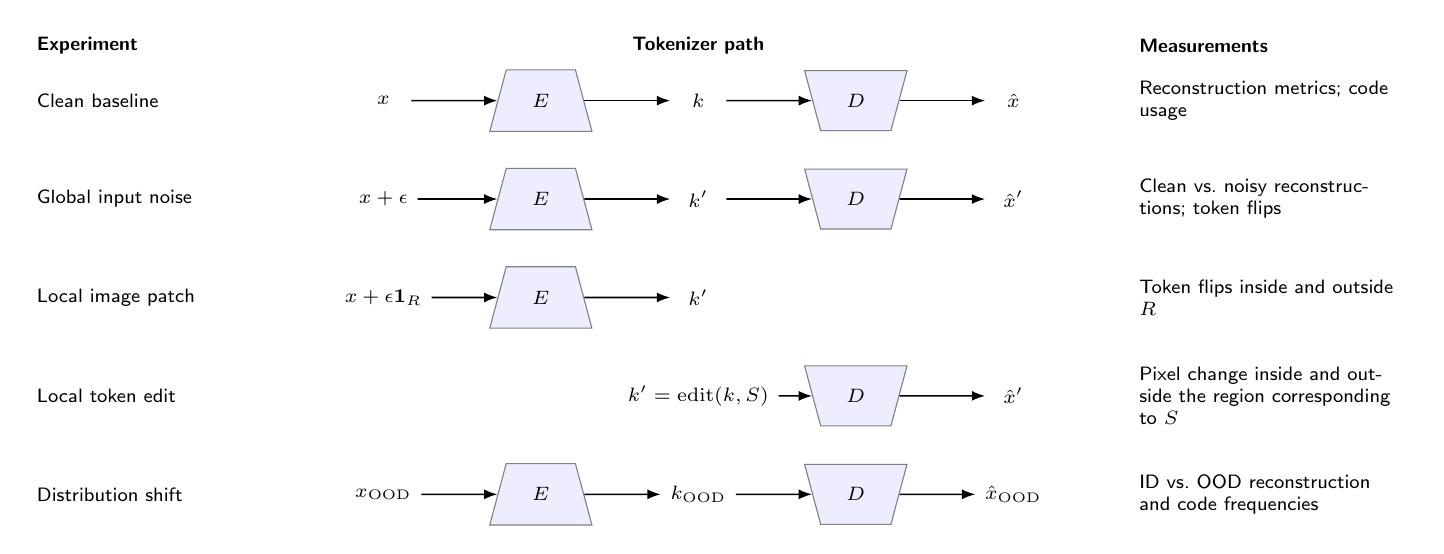
\begin{tikzpicture}[
    font=\sffamily\scriptsize,
    data/.style={align=center, minimum width=7mm},
    stage/.style={draw=black!50, trapezium, trapezium angle=75,
        minimum width=13mm, minimum height=7mm, fill=blue!7},
    flow/.style={-{Latex[length=1.7mm]}, semithick},
    note/.style={align=left, text width=34mm}
]
\node[note, font=\sffamily\bfseries\scriptsize] at (-27mm,7mm) {Experiment};
\node[font=\sffamily\bfseries\scriptsize] at (40mm,7mm) {Tokenizer path};
\node[note, font=\sffamily\bfseries\scriptsize] at (113mm,7mm) {Measurements};
\foreach \r/\title/\inputtext/\tokentext/\outputtext in {
  1/Clean baseline/$x$/$k$/$\hat{x}$,
  2/Global input noise/$x+\epsilon$/$k'$/$\hat{x}'$,
  5/Distribution shift/$x_{\mathrm{OOD}}$/$k_{\mathrm{OOD}}$/$\hat{x}_{\mathrm{OOD}}$}{
    \pgfmathsetmacro{\yy}{-(\r-1)*1.25}
    \node[note] at (-27mm,\yy) {\title};
    \node[data] (x\r) at (0,\yy) {\inputtext};
    \node[stage] (e\r) at (20mm,\yy) {$E$};
    \node[data] (k\r) at (40mm,\yy) {\tokentext};
    \node[stage, trapezium angle=105] (d\r) at (60mm,\yy) {$D$};
    \node[data] (o\r) at (80mm,\yy) {\outputtext};
    \draw[flow] (x\r) -- (e\r);
    \draw[flow] (e\r) -- (k\r);
    \draw[flow] (k\r) -- (d\r);
    \draw[flow] (d\r) -- (o\r);
}
\node[note] at (-27mm,-2.5) {Local image patch};
\node[data] (x3) at (0,-2.5) {$x+\epsilon\mathbf{1}_{R}$};
\node[stage] (e3) at (20mm,-2.5) {$E$};
\node[data] (k3) at (40mm,-2.5) {$k'$};
\draw[flow] (x3) -- (e3);
\draw[flow] (e3) -- (k3);
\node[note] at (-27mm,-3.75) {Local token edit};
\node[data] (k4) at (40mm,-3.75) {$k'=\operatorname{edit}(k,S)$};
\node[stage, trapezium angle=105] (d4) at (60mm,-3.75) {$D$};
\node[data] (o4) at (80mm,-3.75) {$\hat{x}'$};
\draw[flow] (k4) -- (d4);
\draw[flow] (d4) -- (o4);
\node[note] at (113mm,0) {Reconstruction metrics; code usage};
\node[note] at (113mm,-1.25) {Clean vs.\ noisy reconstructions; token flips};
\node[note] at (113mm,-2.5) {Token flips inside and outside $R$};
\node[note] at (113mm,-3.75) {Pixel change inside and outside the region corresponding to $S$};
\node[note] at (113mm,-5) {ID vs.\ OOD reconstruction and code frequencies};
\end{tikzpicture}
}
    \caption{Overview of the five stages of the study. Reconstruction metrics are
    computed between images, token flips are computed between token grids, and
    the local experiments measure responses both inside and outside the intervened
    region.}
    \label{fig:tokenizer_probe_taxonomy}
\end{figure}

\section{Thesis Outline}
\label{sec:thesis_outline}

The thesis is structured as follows. Chapter~\ref{ch:background} introduces
autoregressive image modeling and vector-quantized tokenizers.
Chapter~\ref{ch:datasets_models_metrics} defines the evaluated models,
datasets, and metrics. Chapters~\ref{ch:rq1}--\ref{ch:rq5} address the five
research questions in sequence. Chapter~\ref{ch:conclusion} summarizes the
results and discusses the study's limitations and future work.

\chapter{Background}
\label{ch:background}

% For AI-assisted explanatory figures in this chapter, use \aifigurecaption{...}
% so the standardized disclosure is included directly in the caption.

This chapter introduces autoregressive image modeling and vector quantization,
then describes early and recent image tokenizers.

\section{Autoregressive Models: From Text to Images}
\label{sec:ar_models_text_to_images}

An autoregressive model represents a joint distribution by predicting each
element from those that precede it. A token is a discrete text unit, such as a
word or subword, drawn from a finite vocabulary. Let
$s=(s_1,\ldots,s_T)$ be a sequence of tokens, where $s_i$ is the token at
position $i$ and $T$ is the sequence length. The chain rule gives
\begin{equation}
    p(s)=\prod_{i=1}^{T}p(s_i\mid s_{<i}),
    \qquad s_{<i}=(s_1,\ldots,s_{i-1}).
\end{equation}
This factorization has long been used for statistical language
modeling~\cite{bengio2003neural}. A text tokenizer converts text into a sequence
of tokens drawn from a finite vocabulary, and a language model learns the
conditional distribution of the next token. Transformers made this approach
effective at scale by using self-attention to model dependencies between
tokens~\cite{vaswani2017attention}. Later work found that language-model loss
follows empirical power laws as the amount of data, model size, and training
compute increase~\cite{kaplan2020scaling}. Large autoregressive language models
then demonstrated broad capabilities under the same training
objective~\cite{brown2020language,touvron2023llama}.

Applying the same principle to images is less direct. An image is a
two-dimensional array rather than an ordered sequence, so an autoregressive
model must first choose both a prediction unit and an ordering. The most literal
choice is to discretize pixel intensities and traverse them in raster order,
from left to right and top to bottom. Early works such as PixelRNN and PixelCNN
showed that this produces tractable image likelihoods and coherent
samples~\cite{oord2016pixel}. Image Transformer later applied self-attention to
autoregressive pixel generation while restricting attention to local
neighborhoods to control its cost~\cite{parmar2018image}.

Pixel-level modeling is conceptually simple but computationally demanding. A
$256\times256$ RGB image contains $196{,}608$ channel values, and generation
must resolve low-level color statistics as well as long-range structure.
Moreover, full self-attention on a sequence of length $T$ has
$\mathcal{O}(T^2)$ time and memory cost. A learned image tokenizer addresses
both problems by mapping the image to a shorter grid of discrete symbols. The
token grids studied in this thesis are flattened in raster order. Tokenization
reduces the number of prediction units but does not choose a different
ordering. Figure~\ref{fig:pixel_vs_token_sequence} contrasts the resulting
sequence lengths.

\begin{figure}[t]
    \centering
    \resizebox{0.94\textwidth}{!}{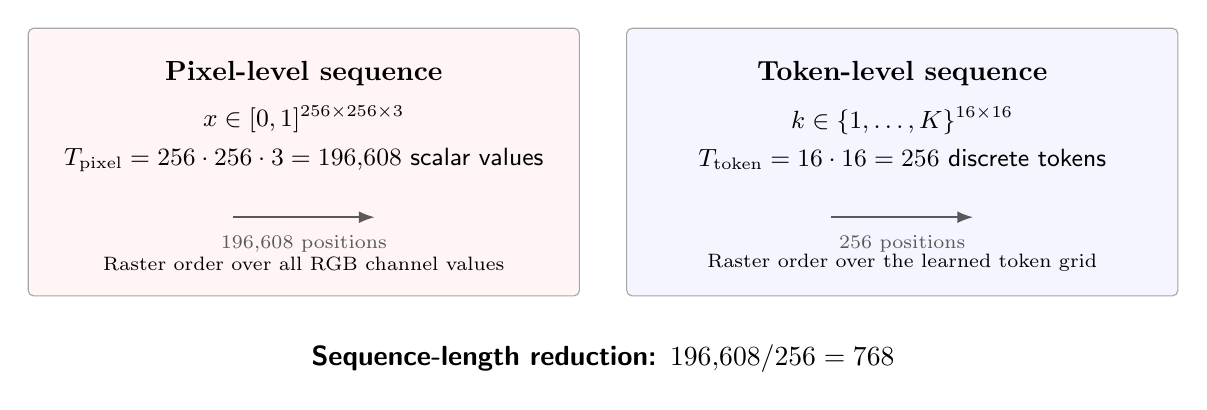
\begin{tikzpicture}[
    font=\sffamily\small,
    panel/.style={draw=black!35, rounded corners=2pt, minimum width=70mm,
                  minimum height=34mm, align=center, inner sep=6pt},
    sequence/.style={draw=black!55, minimum height=5mm, minimum width=7mm,
                     inner sep=0pt},
    arrow/.style={-{Latex[length=2mm]}, semithick, black!65}
]
\node[panel, fill=red!4] (pixels) at (-38mm,0) {};
\node[font=\bfseries, anchor=north] at ([yshift=-3mm]pixels.north)
    {Pixel-level sequence};
\node[align=center] (pixelshape) at ([yshift=3mm]pixels.center)
    {$x\in[0,1]^{256\times256\times3}$\\[1mm]
     $T_{\mathrm{pixel}}=256\cdot256\cdot3=196{,}608$ scalar values};
\node[anchor=south, align=center, font=\scriptsize] at ([yshift=2mm]pixels.south)
    {Raster order over all RGB channel values};

\node[panel, fill=blue!4] (tokens) at (38mm,0) {};
\node[font=\bfseries, anchor=north] at ([yshift=-3mm]tokens.north)
    {Token-level sequence};
\node[align=center] (tokenshape) at ([yshift=3mm]tokens.center)
    {$k\in\{1,\ldots,K\}^{16\times16}$\\[1mm]
     $T_{\mathrm{token}}=16\cdot16=256$ discrete tokens};
\node[anchor=south, align=center, font=\scriptsize] at ([yshift=2mm]tokens.south)
    {Raster order over the learned token grid};

\draw[arrow] ([xshift=-9mm,yshift=-7mm]pixels.center) --
    node[below=1mm, font=\scriptsize] {$196{,}608$ positions}
    ([xshift=9mm,yshift=-7mm]pixels.center);
\draw[arrow] ([xshift=-9mm,yshift=-7mm]tokens.center) --
    node[below=1mm, font=\scriptsize] {$256$ positions}
    ([xshift=9mm,yshift=-7mm]tokens.center);

\node[font=\sffamily\bfseries] at (0,-25mm)
    {Sequence-length reduction: $196{,}608/256=768$};
\end{tikzpicture}
}
    \caption{Pixel-level flattening produces much longer autoregressive sequences than token-level flattening. A learned tokenizer replaces groups of pixel values with discrete visual symbols.}
    \label{fig:pixel_vs_token_sequence}
\end{figure}

Autoregressive image generation therefore has two stages, illustrated in
Figure~\ref{fig:two_stage_autoregressive_pipeline}. A tokenizer first converts
images into compact token grids and reconstructs images from them. An
autoregressive model is then trained on the resulting token sequences. This
second-stage model is also called a \emph{prior}: it models the distribution of
token sequences and can sample a sequence for the decoder.

\begin{figure}[t]
    \centering
    \resizebox{0.96\textwidth}{!}{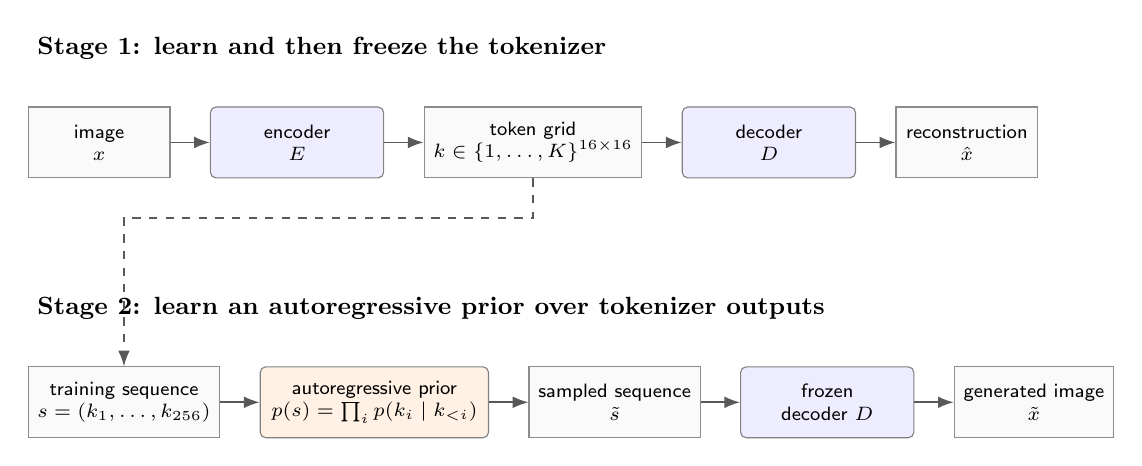
\begin{tikzpicture}[
    font=\sffamily\scriptsize,
    block/.style={draw=black!50, rounded corners=2pt, minimum width=22mm,
                  minimum height=9mm, align=center, fill=blue!7},
    data/.style={draw=black!45, minimum width=18mm, minimum height=9mm,
                 align=center, fill=black!2},
    prior/.style={block, fill=orange!10, minimum width=29mm},
    arrow/.style={-{Latex[length=2mm]}, semithick, black!65}
]
\node[font=\bfseries\small, anchor=west] (s1) at (-75mm,15mm)
    {Stage 1: learn and then freeze the tokenizer};
\node[data, anchor=west] (x) at (-75mm,3mm) {image\\$x$};
\node[block, right=5mm of x] (enc) {encoder\\$E$};
\node[data, right=5mm of enc] (grid) {token grid\\$k\in\{1,\ldots,K\}^{16\times16}$};
\node[block, right=5mm of grid] (dec) {decoder\\$D$};
\node[data, right=5mm of dec] (recon) {reconstruction\\$\hat{x}$};
\draw[arrow] (x) -- (enc);
\draw[arrow] (enc) -- (grid);
\draw[arrow] (grid) -- (dec);
\draw[arrow] (dec) -- (recon);

\node[font=\bfseries\small, anchor=west] (s2) at (-75mm,-18mm)
    {Stage 2: learn an autoregressive prior over tokenizer outputs};
\node[data, anchor=west] (trainseq) at (-75mm,-30mm)
    {training sequence\\$s=(k_1,\ldots,k_{256})$};
\node[prior, right=5mm of trainseq] (ar)
    {autoregressive prior\\$p(s)=\prod_i p(k_i\mid k_{<i})$};
\node[data, right=5mm of ar] (sample)
    {sampled sequence\\$\tilde{s}$};
\node[block, right=5mm of sample] (dec2) {frozen\\decoder $D$};
\node[data, right=5mm of dec2] (generated) {generated image\\$\tilde{x}$};
\draw[arrow] (trainseq) -- (ar);
\draw[arrow] (ar) -- (sample);
\draw[arrow] (sample) -- (dec2);
\draw[arrow] (dec2) -- (generated);
\draw[arrow, dashed] (grid.south) -- ++(0,-5mm) -| (trainseq.north);
\end{tikzpicture}
}
    \caption{Two-stage autoregressive image generation. The tokenizer maps an image to a compact token grid; an autoregressive prior models the flattened token sequence; the tokenizer decoder maps sampled tokens back to image space.}
    \label{fig:two_stage_autoregressive_pipeline}
\end{figure}

Image tokenizers may use convolutions, attention, or both. Their function is to
represent images with discrete tokens and reconstruct images from them. The
autoregressive model has a different function: it predicts those tokens in
sequence. The tokenizer determines which image information reaches that model,
the sequence length, and the vocabulary used for next-token prediction.

\section{Image Tokens and Vector Quantization}
\label{sec:image_tokens_vq}

Vector quantization replaces continuous feature vectors with entries from a
finite codebook. We introduce this operation using VQ-VAE, which learns
discrete latent representations by assigning encoder outputs to a learned
codebook~\cite{oord2017neural}. A separate autoregressive model can then model
the resulting token sequence. VQ-VAE-2 later showed that hierarchical discrete
latents and stronger priors could support high-fidelity large-scale image
generation~\cite{razavi2019vqvae2}.

VQ-VAE contains an encoder, a vector quantizer, and a decoder. Given an input
image $x\in\mathbb{R}^{H\times W\times C}$, the encoder produces a continuous
feature grid $z_e(x)\in\mathbb{R}^{h\times w\times d}$. The full path is shown
in Figure~\ref{fig:vqvae_pipeline}.

\begin{figure}[t]
    \centering
    \resizebox{0.9\textwidth}{!}{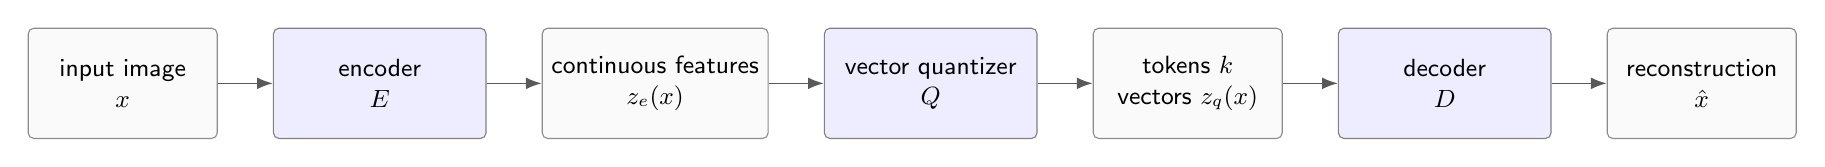
\begin{tikzpicture}[
    font=\sffamily\small,
    data/.style={draw=black!45, rounded corners=2pt, fill=black!2,
                 minimum width=24mm, minimum height=14mm, align=center},
    block/.style={draw=black!50, rounded corners=2pt, fill=blue!7,
                  minimum width=27mm, minimum height=14mm, align=center},
    arrow/.style={-{Latex[length=2mm]}, semithick, black!65}
]
\node[data] (input) {input image\\$x$};
\node[block, right=7mm of input] (encoder) {encoder\\$E$};
\node[data, right=7mm of encoder] (features) {continuous features\\$z_e(x)$};
\node[block, right=7mm of features] (quantizer) {vector quantizer\\$Q$};
\node[data, right=7mm of quantizer] (tokens) {tokens $k$\\vectors $z_q(x)$};
\node[block, right=7mm of tokens] (decoder) {decoder\\$D$};
\node[data, right=7mm of decoder] (output) {reconstruction\\$\hat{x}$};
\draw[arrow] (input) -- (encoder);
\draw[arrow] (encoder) -- (features);
\draw[arrow] (features) -- (quantizer);
\draw[arrow] (quantizer) -- (tokens);
\draw[arrow] (tokens) -- (decoder);
\draw[arrow] (decoder) -- (output);
\end{tikzpicture}
}
    \aifigurecaption{VQ-VAE representation path. The encoder produces continuous
    features, the vector quantizer returns integer tokens and their associated
    codebook vectors, and the decoder reconstructs the image. Based on van den
    Oord et al.~\cite{oord2017neural}.}
    \label{fig:vqvae_pipeline}
\end{figure}

At each spatial position $(u,v)$, the vector $z_e(x)_{u,v}\in\mathbb{R}^{d}$ is assigned to its nearest entry in a learned codebook
$\mathcal{E}=\{e_1,\ldots,e_K\}$, where $e_j\in\mathbb{R}^{d}$. Quantization produces an integer token grid $k\in\{1,\ldots,K\}^{h\times w}$ and a quantized latent tensor $z_q(x)\in\mathbb{R}^{h\times w\times d}$:
\begin{align}
    z_e(x) &= E(x), \\
    k_{u,v} &= \underset{j\in\{1,\ldots,K\}}{\arg\min}\,
        \lVert z_e(x)_{u,v}-e_j\rVert_2, \\
    z_q(x)_{u,v} &= e_{k_{u,v}}, \\
    \hat{x} &= D\!\left(z_q(x)\right).
\end{align}
Here, $D$ is the decoder and $\hat{x}$ is the reconstruction. Figure~\ref{fig:vq_clustering_codebook} gives the corresponding geometric interpretation: codebook entries act as learned representative points in latent space.

\begin{figure}[t]
    \centering
    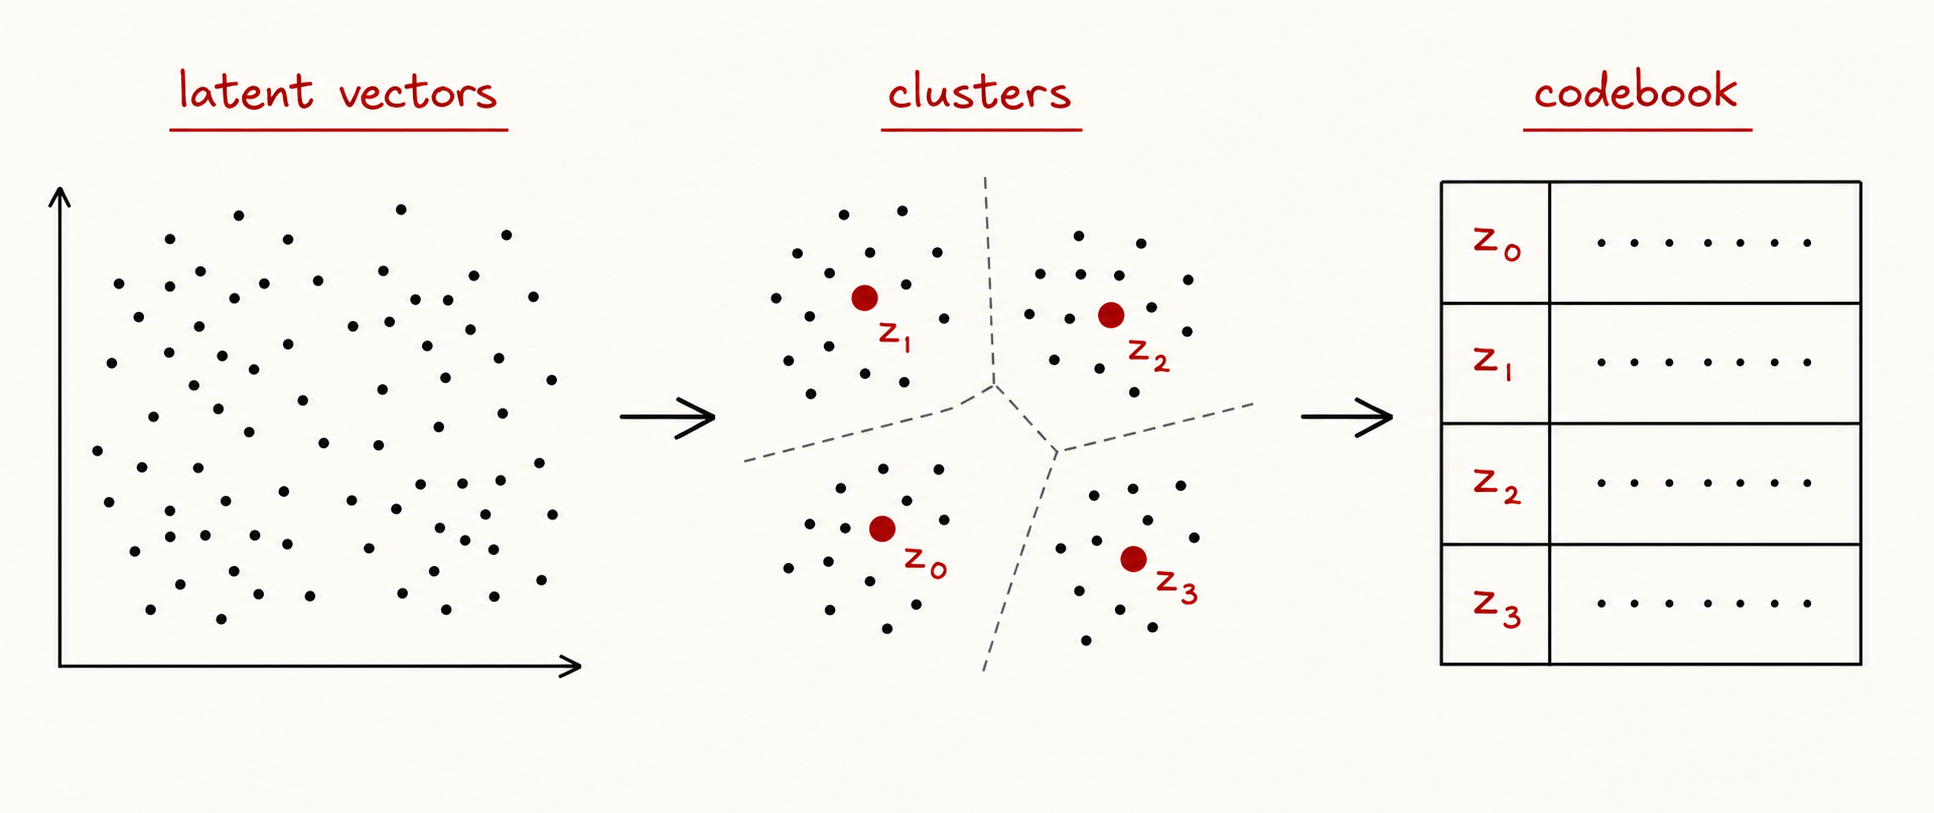
\includegraphics[width=0.94\textwidth]{ch02_fig_2_2a_vq_clustering_codebook.png}
    \aifigurecaption{Vector quantization as clustering in latent space. Continuous encoder outputs are assigned to their nearest learned codebook entry, and the entry index becomes a discrete token.}
    \label{fig:vq_clustering_codebook}
\end{figure}

The decoder receives $z_q(x)$ rather than the continuous encoder output. Image information must therefore pass through a finite vocabulary of $K$ vectors. The same representation has two roles: the quantized vectors are the decoder input, while their integer indices form the discrete sequence modeled by the autoregressive prior. Figure~\ref{fig:feature_map_to_token_sequence} summarizes this conversion.

\begin{figure}[t]
    \centering
    \resizebox{0.94\textwidth}{!}{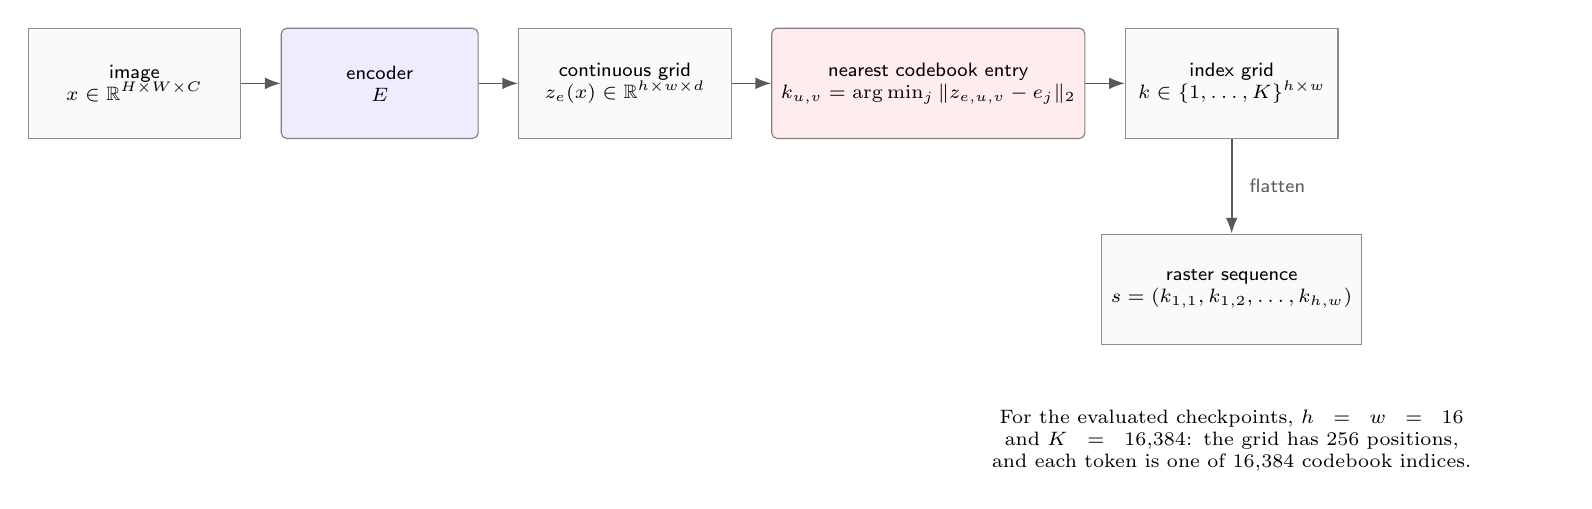
\begin{tikzpicture}[
    font=\sffamily\scriptsize,
    block/.style={draw=black!50, rounded corners=2pt, minimum width=25mm,
                  minimum height=14mm, align=center, fill=blue!7},
    data/.style={draw=black!45, minimum width=27mm, minimum height=14mm,
                 align=center, fill=black!2},
    quant/.style={block, fill=red!7, minimum width=31mm},
    arrow/.style={-{Latex[length=2mm]}, semithick, black!65}
]
\node[data] (image) at (-66mm,0) {image\\$x\in\mathbb{R}^{H\times W\times C}$};
\node[block, right=5mm of image] (encoder) {encoder\\$E$};
\node[data, right=5mm of encoder] (latent)
    {continuous grid\\$z_e(x)\in\mathbb{R}^{h\times w\times d}$};
\node[quant, right=5mm of latent] (nearest)
    {nearest codebook entry\\$k_{u,v}=\arg\min_j\|z_{e,u,v}-e_j\|_2$};
\node[data, right=5mm of nearest] (indices)
    {index grid\\$k\in\{1,\ldots,K\}^{h\times w}$};
\node[data, below=12mm of indices] (sequence)
    {raster sequence\\$s=(k_{1,1},k_{1,2},\ldots,k_{h,w})$};
\draw[arrow] (image) -- (encoder);
\draw[arrow] (encoder) -- (latent);
\draw[arrow] (latent) -- (nearest);
\draw[arrow] (nearest) -- (indices);
\draw[arrow] (indices) -- node[right=1mm] {flatten} (sequence);
\node[below=7mm of sequence, align=center, font=\scriptsize, text width=82mm]
    {For the evaluated checkpoints, $h=w=16$ and $K=16{,}384$: the grid has
     $256$ positions, and each token is one of $16{,}384$ codebook indices.};
\end{tikzpicture}
}
    \caption{From a continuous feature map to a discrete sequence. The encoder produces a latent grid, vector quantization replaces each latent vector with a codebook index, and the token grid is flattened for sequence modeling.}
    \label{fig:feature_map_to_token_sequence}
\end{figure}

\subsection{Learning the Discrete Representation}

VQ-VAE is trained by gradient descent, but nearest-neighbor assignment is not
differentiable. It therefore uses a straight-through estimator. During the
forward pass the decoder receives quantized vectors; during backpropagation,
the gradient with respect to the quantized representation is copied to the
encoder output~\cite{bengio2013estimating,oord2017neural}. The encoder, decoder,
and codebook are learned together.

The objective contains a reconstruction loss and two additional terms for
learning the codebook and encoder representation:
\begin{equation}
    \mathcal{L}_{\mathrm{VQ}}
    =
    \underbrace{-\log p\!\left(x\mid z_q(x)\right)}_{\mathcal{L}_{\mathrm{rec}}}
    + \underbrace{\left\lVert \operatorname{sg}[z_e(x)]-z_q(x)\right\rVert_2^2}_{\mathcal{L}_{\mathrm{cod}}}
    + \underbrace{\beta\left\lVert z_e(x)-\operatorname{sg}[z_q(x)]\right\rVert_2^2}_{\mathcal{L}_{\mathrm{comm}}}.
\end{equation}
The reconstruction term follows the likelihood convention in the original
VQ-VAE formulation~\cite{oord2017neural}. The stop-gradient operator
$\operatorname{sg}[\cdot]$ is the identity in the forward pass and has zero
derivative. The codebook term $\mathcal{L}_{\mathrm{cod}}$ moves embeddings
toward encoder outputs. The commitment term $\mathcal{L}_{\mathrm{comm}}$
keeps encoder outputs close to their assigned embeddings.

The codebook contains $K$ entries, but a dataset may activate only a subset.
Codebook collapse occurs when many entries receive few or no assignments, which
reduces the empirical vocabulary available to the autoregressive
model~\cite{lancucki2020robust,yu2021vector,mentzer2023finite}. Chapter~\ref{ch:rq1}
measures nominal and empirical vocabulary directly.

Nearest-neighbor assignment also partitions latent space into discrete regions.
A small change in an encoder output can cross a region boundary and change its
token abruptly, as illustrated in Figure~\ref{fig:vq_boundary_crossing}.

\begin{figure}[t]
    \centering
    \resizebox{0.9\textwidth}{!}{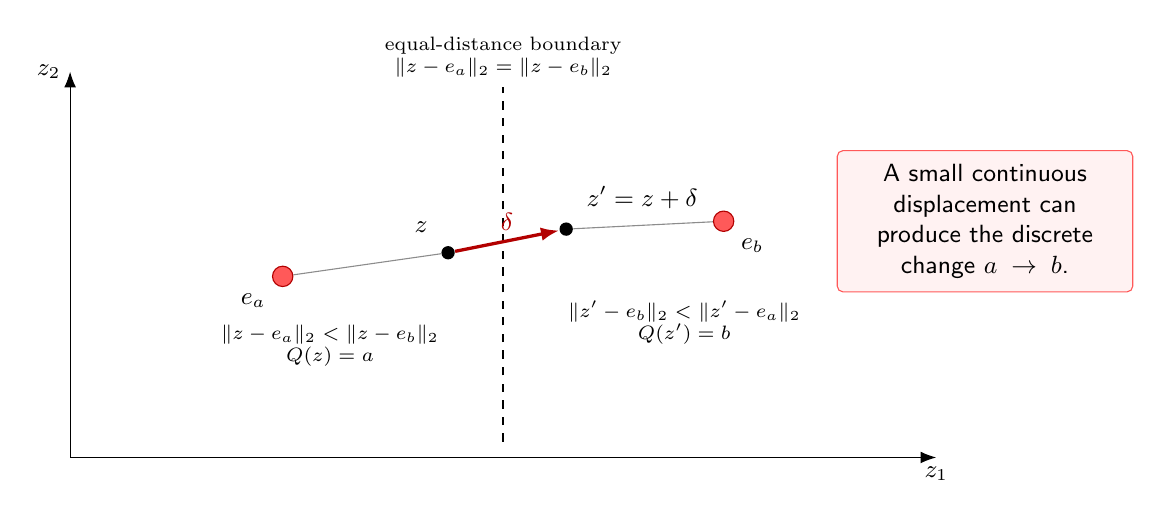
\begin{tikzpicture}[
    font=\sffamily\small,
    point/.style={circle, fill=black, inner sep=1.7pt},
    centroid/.style={circle, draw=red!70!black, fill=red!65, inner sep=2.6pt},
    move/.style={-{Latex[length=2.3mm]}, very thick, red!70!black}
]
\draw[-{Latex[length=2mm]}] (-55mm,-24mm) -- (55mm,-24mm)
    node[below] {$z_1$};
\draw[-{Latex[length=2mm]}] (-55mm,-24mm) -- (-55mm,25mm)
    node[left] {$z_2$};
\draw[dashed, semithick] (0,-22mm) -- (0,23mm)
    node[above, align=center, font=\scriptsize] {equal-distance boundary\\$\|z-e_a\|_2=\|z-e_b\|_2$};
\node[centroid, label=below left:$e_a$] (ea) at (-28mm,-1mm) {};
\node[centroid, label=below right:$e_b$] (eb) at (28mm,6mm) {};
\node[point] (before) at (-7mm,2mm) {};
\node[above left=1mm of before] {$z$};
\node[point] (after) at (8mm,5mm) {};
\node[above right=1mm of after] {$z'=z+\delta$};
\draw[move] (before) -- node[above] {$\delta$} (after);
\draw[thin, black!45] (before) -- (ea);
\draw[thin, black!45] (after) -- (eb);
\node[align=center, below=7mm of before, xshift=-15mm, font=\scriptsize]
    {$\|z-e_a\|_2<\|z-e_b\|_2$\\$Q(z)=a$};
\node[align=center, below=7mm of after, xshift=15mm, font=\scriptsize]
    {$\|z'-e_b\|_2<\|z'-e_a\|_2$\\$Q(z')=b$};
\node[draw=red!65, rounded corners=2pt, fill=red!5, align=center,
      right=13mm of eb, text width=34mm, inner sep=5pt]
    {A small continuous displacement can produce the discrete change $a\rightarrow b$.};
\end{tikzpicture}
}
    \caption{Nearest-neighbor regions create discontinuities in latent space. A small displacement of an encoder output can cross a quantization boundary and change its assigned token.}
    \label{fig:vq_boundary_crossing}
\end{figure}

\section{VQGAN and Taming Transformers}
\label{sec:vqgan_taming}

VQ-VAE showed how to learn a discrete token space that an autoregressive model
can model, with a decoder that converts sampled token sequences into
images~\cite{oord2017neural}. Its reconstruction objective, however, does not
necessarily preserve perceptually important high-frequency detail. When several
sharp reconstructions are plausible, minimizing an average pixel error can
favor a blurred result. Esser et al.\ address this limitation with a
vector-quantized generative adversarial network, commonly called VQGAN, and use
its discrete representation to make transformer-based high-resolution
synthesis practical~\cite{esser2021taming}.

VQGAN retains the encoder--quantizer--decoder structure of VQ-VAE but changes
the training objective. In the implementation used by the evaluated VQGAN
checkpoint, the generator objective has four components:
\begin{equation}
    \mathcal{L}_{\mathrm{VQGAN}}
    =
    \mathcal{L}_{\mathrm{rec}}
    + \mathcal{L}_{\mathrm{perc}}
    + \lambda\,\mathcal{L}_{\mathrm{adv}}
    + \mathcal{L}_{\mathrm{codebook}}.
\end{equation}
This expanded implementation view separates the pixel reconstruction,
perceptual, adversarial, and codebook terms; their configured and adaptive
weights are omitted here for readability. The perceptual term compares
activations of a pretrained network rather than requiring exact pixel
agreement. A patch-based discriminator supplies the adversarial term. These
objectives encourage the decoder to preserve perceptually salient structure and
synthesize plausible fine detail. Figure~\ref{fig:adversarial_and_perceptual_losses}
shows how the losses supervise the reconstructed image.

\begin{figure}[t]
    \centering
    \resizebox{0.94\textwidth}{!}{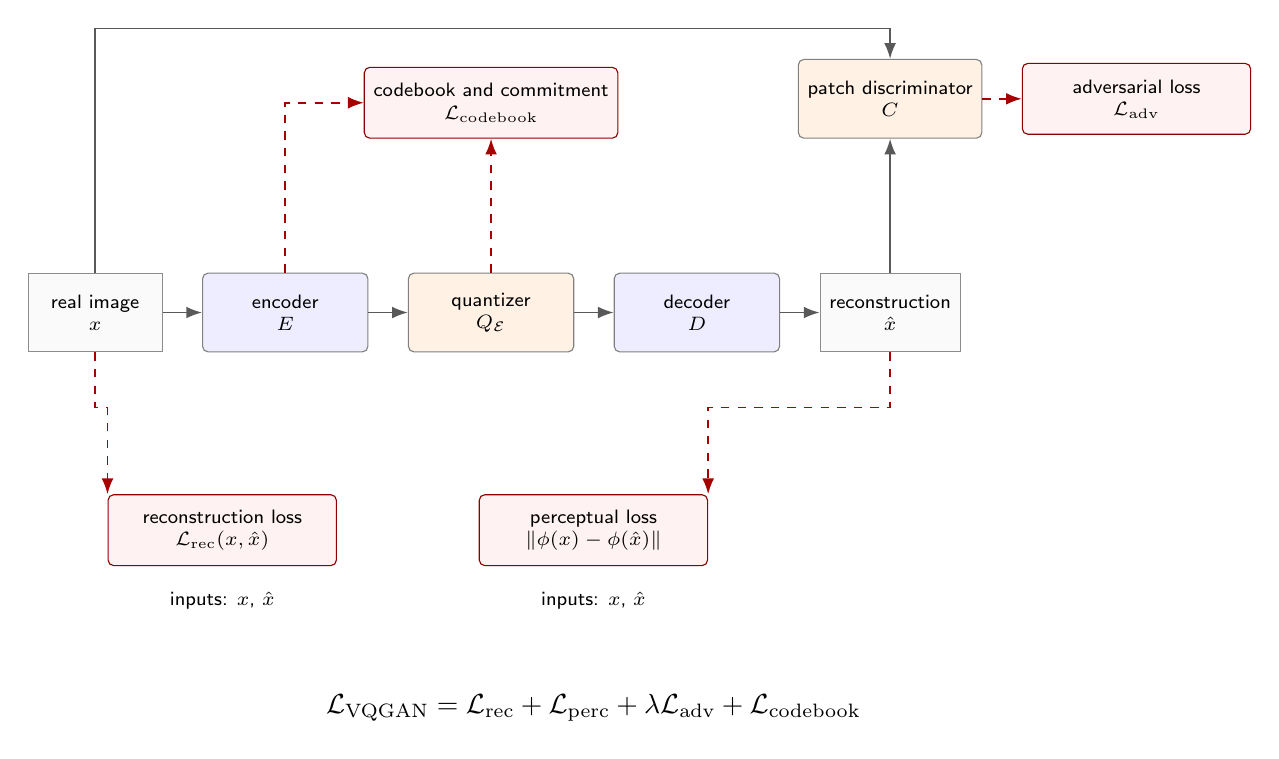
\begin{tikzpicture}[
    font=\sffamily\scriptsize,
    block/.style={draw=black!50, rounded corners=2pt, minimum width=21mm,
                  minimum height=10mm, align=center, fill=blue!7},
    data/.style={draw=black!45, minimum width=17mm, minimum height=10mm,
                 align=center, fill=black!2},
    loss/.style={draw=red!55!black, rounded corners=2pt, minimum width=29mm,
                 minimum height=9mm, align=center, fill=red!5},
    arrow/.style={-{Latex[length=2mm]}, semithick, black!65},
    supervise/.style={-{Latex[length=2mm]}, dashed, semithick, red!65!black}
]
\node[data] (x) at (-68mm,0) {real image\\$x$};
\node[block, right=5mm of x] (enc) {encoder\\$E$};
\node[block, right=5mm of enc, fill=orange!10] (quant) {quantizer\\$Q_{\mathcal E}$};
\node[block, right=5mm of quant] (dec) {decoder\\$D$};
\node[data, right=5mm of dec] (xhat) {reconstruction\\$\hat{x}$};
\draw[arrow] (x) -- (enc);
\draw[arrow] (enc) -- (quant);
\draw[arrow] (quant) -- (dec);
\draw[arrow] (dec) -- (xhat);

\node[loss, below=18mm of enc, xshift=-8mm] (rec)
    {reconstruction loss\\$\mathcal L_{\mathrm{rec}}(x,\hat{x})$};
\node[loss, below=18mm of quant, xshift=13mm] (perc)
    {perceptual loss\\$\|\phi(x)-\phi(\hat{x})\|$};
\node[block, above=17mm of xhat, fill=orange!10] (disc)
    {patch discriminator\\$C$};
\node[loss, right=5mm of disc] (adv)
    {adversarial loss\\$\mathcal L_{\mathrm{adv}}$};
\node[loss, above=17mm of quant] (codebook)
    {codebook and commitment\\$\mathcal L_{\mathrm{codebook}}$};

\draw[supervise] (x.south) -- ++(0,-7mm) -| (rec.north west);
\draw[supervise] (xhat.south) -- ++(0,-7mm) -| (perc.north east);
\node[below=2mm of rec, align=center] {inputs: $x$, $\hat{x}$};
\node[below=2mm of perc, align=center] {inputs: $x$, $\hat{x}$};
\draw[arrow] (x.north) -- ++(0,31mm) -| (disc.north);
\draw[arrow] (xhat.north) -- (disc.south);
\draw[supervise] (disc) -- (adv);
\draw[supervise] (enc.north) |- (codebook.west);
\draw[supervise] (quant.north) -- (codebook.south);

\node[below=15mm of perc, align=center, font=\sffamily\bfseries]
    {$\mathcal L_{\mathrm{VQGAN}}=\mathcal L_{\mathrm{rec}}+\mathcal L_{\mathrm{perc}}
     +\lambda\mathcal L_{\mathrm{adv}}+\mathcal L_{\mathrm{codebook}}$};
\end{tikzpicture}
}
    \caption{VQGAN training combines reconstruction, perceptual, and adversarial supervision. Reconstruction and perceptual losses compare the input and reconstruction, while a patch discriminator encourages locally realistic outputs.}
    \label{fig:adversarial_and_perceptual_losses}
\end{figure}

The first-stage model is convolutional, with non-local attention at its lowest-resolution level. This architecture combines local feature extraction with a limited mechanism for contextual interaction before quantization. Once trained, the tokenizer is frozen and images are represented by their codebook indices. A transformer is then trained autoregressively on the resulting sequences. The original architecture is reproduced in Figure~\ref{fig:vqgan_first_stage_model}.

\begin{figure}[t]
    \centering
    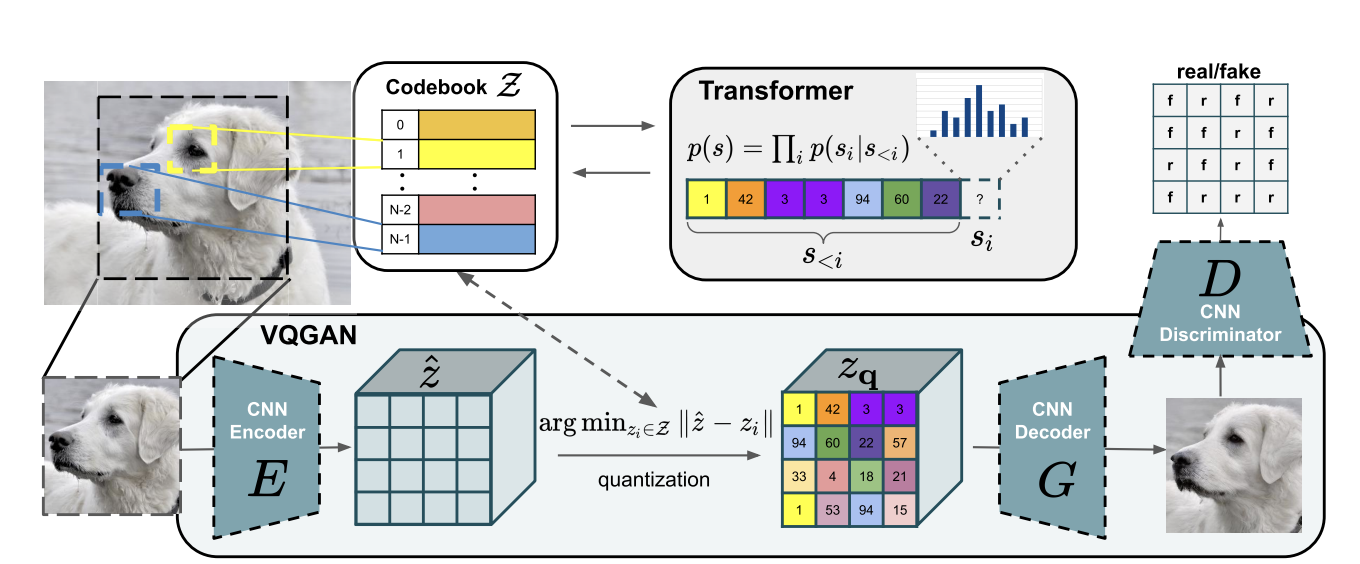
\includegraphics[width=0.94\textwidth]{ch02_taming_transformers_architecture.png}
    \caption{Taming Transformers architecture, comprising the VQGAN tokenizer, learned codebook, autoregressive transformer, and patch discriminator. Reproduced from Esser et al.~\cite{esser2021taming}.}
    \label{fig:vqgan_first_stage_model}
\end{figure}

A smaller token grid reduces the sequence length processed by the transformer,
but forces each token to carry more image information and can reduce
reconstruction fidelity. Esser et al.\ study this trade-off through different
codebook sizes and latent resolutions~\cite{esser2021taming}.

\section{\texorpdfstring{\mbox{LlamaGen}}{LlamaGen}}
\label{sec:llamagen_tokenizer}

After VQGAN, subsequent work improved autoregressive image generation. DALL-E,
for example, models text and image tokens as a single autoregressive
stream~\cite{ramesh2021zero}.

LlamaGen revisits this approach using a Llama-style transformer and reports
competitive results against diffusion baselines through tokenizer and model
design~\cite{sun2024llamagen}. The system preserves the two-stage design: a
vector-quantized tokenizer converts images to discrete grids, and an
autoregressive model predicts their tokens.

A large nominal codebook is of limited value if the tokenizer uses only a small
fraction of its entries. LlamaGen addresses this problem with low-dimensional
codebook embeddings and L2-normalized lookup~\cite{sun2024llamagen}. Reducing
the embedding dimension makes nearest-neighbor assignment less sparse, while
normalization places encoder projections and codebook entries on a common unit
sphere before assignment. LlamaGen also evaluates longer token sequences as a
separate design choice. This thesis evaluates its VQ-16 tokenizer.

\section{Representation Properties Beyond Reconstruction Quality}
\label{sec:reconstruction_to_behavior}

A tokenizer is usually evaluated first through reconstruction: given $x$, it produces
$\hat{x}=D(Q(E(x)))$, and the two images are compared. Reconstruction is essential because any information discarded by the tokenizer is unavailable to the generative model. It is not, however, a complete description of the induced discrete representation.

The tokenizer also determines the effective vocabulary, token frequencies, and
spatial response to perturbations. Two tokenizers with similar reconstruction
quality may use different fractions of their codebooks. A small image
perturbation may leave one token grid largely unchanged while altering many
entries in another. A local token edit may remain local or propagate through
the decoder. Chapters~\ref{ch:rq1}, \ref{ch:rq3}, and \ref{ch:rq4} measure these
properties because the autoregressive model learns the distribution created by
the tokenizer rather than the original pixel distribution directly.

VQGAN and LlamaGen represent two stages in the development of discrete image
tokenization. Both learn a finite visual vocabulary and expose token grids to
an autoregressive model, but they differ in tokenizer design and in the
empirical distributions induced over their vocabularies. Their comparison
separates behavior shared by vector-quantized tokenizers from behavior tied to
a particular design.

\chapter{Datasets, Models, and Metrics}
\label{ch:datasets_models_metrics}

% For AI-assisted explanatory figures in this chapter, use \aifigurecaption{...}
% so the standardized disclosure is included directly in the caption.

This work focuses on two pretrained image tokenizers: VQGAN
~\cite{esser2021taming} and LlamaGen VQ-16~\cite{sun2024llamagen}. This chapter
defines these two tokenizers, the evaluation datasets, and the metrics used to
measure reconstruction quality, codebook use, and spatial behavior.

\section{Models Under Study}
\label{sec:models_under_study}

These two tokenizers share the same external task, mapping $256\times256$
images to discrete token grids. They use the same VQGAN-style convolutional
encoder--decoder backbone, while their quantizer projections, codebook
geometry, and training recipes differ~\cite{esser2021taming,sun2024llamagen}.

VQGAN uses an encoder, vector quantizer, and decoder with a convolutional
architecture and attention at the lowest-resolution level
~\cite{esser2021taming}. Section~\ref{sec:vqgan_taming} describes the model in
more detail. The pretrained version used in this study was trained with a
reconstruction, perceptual, adversarial, and codebook objective. It has a
downsampling factor $f=16$, so a $256\times256$ image becomes a $16\times16$
token grid. Its codebook has $K=16{,}384$ entries with dimension $256$.

LlamaGen provides two pretrained versions, VQ-16 and VQ-8, with downsampling
factors of 16 and 8, respectively~\cite{sun2024llamagen,llamagengithub}. To
maintain the same token-grid size as VQGAN, these experiments use VQ-16. It maps
$256\times256$ images to a $16\times16$ grid with a nominal codebook of
$K=16{,}384$. Its codebook embeddings have dimension $d=8$. Before
nearest-neighbor lookup, the projected encoder vectors and codebook vectors are
normalized to unit L2 norm.

Table~\ref{tab:model_config_summary} summarizes the configurations of the two
evaluated tokenizers.

\begin{table}[htbp]
    \centering
    \renewcommand{\arraystretch}{1.2}
    \begin{tabularx}{\textwidth}{>{\raggedright\arraybackslash}p{0.22\textwidth} >{\raggedright\arraybackslash}X >{\raggedright\arraybackslash}X}
        \textbf{Property} & \textbf{VQGAN} & \textbf{LlamaGen} \\ \hline
        Source & Taming Transformers~\cite{esser2021taming} & LlamaGen~\cite{sun2024llamagen} \\
        Main tokenizer & ImageNet first stage, $f=16$ & \texttt{VQ-16} \\
        Input resolution & $256\times256$ & $256\times256$ \\
        Token grid & $16\times16$ & $16\times16$ \\
        Encoder/decoder & VQGAN-style convolutional backbone & VQGAN-style convolutional backbone \\
        Nominal codebook size & $K=16{,}384$ & $K=16{,}384$ \\
        Embedding dimension & $256$ & $8$ \\
        Codebook normalization & none & L2-normalized lookup \\
        Training loss components & pixel, perceptual, adversarial, codebook/commitment & pixel, perceptual, adversarial, codebook/commitment \\
    \end{tabularx}
    \caption{Tokenizer configurations compared in the thesis. Both models produce the same token-grid size and nominal vocabulary size and share the encoder--decoder backbone. LlamaGen uses an L2 pixel loss with LPIPS and PatchGAN terms~\cite{sun2024llamagen}; the objectives differ in details and weights, rather than in the presence of perceptual or adversarial supervision.}
    \label{tab:model_config_summary}
\end{table}

\section{Datasets}
\label{sec:datasets}

The ImageNet-1K validation split is used for reconstruction baselines, codebook
usage, global perturbation robustness, and locality experiments. It belongs to
the training domain of both selected checkpoints and appears in their published
evaluations~\cite{esser2021taming,sun2024llamagen}. ImageNet-V2 is also used in
Chapter~\ref{ch:rq4} for decoder locality. Chapter~\ref{ch:rq5} studies
distribution shifts using ImageNet-V2, ImageNet-Sketch, ObjectNet, BloodMNIST,
OrganAMNIST, and RVL-CDIP.

\subsection{ImageNet}
\label{subsec:imagenet_validation}

ImageNet was introduced as a large-scale visual recognition dataset organized around the WordNet noun hierarchy~\cite{deng2009imagenet}. It was collected to provide broad object-category coverage at a scale that earlier recognition datasets did not offer. The ImageNet Large Scale Visual Recognition Challenge (ILSVRC) later standardized a 1,000-class classification benchmark, commonly called ImageNet-1K~\cite{russakovsky2015imagenet}.

ImageNet is a standard reference dataset for the evaluated VQ tokenizers
~\cite{esser2021taming,sun2024llamagen}. We use the ImageNet-1K validation split
because it matches their training domain. It contains 50,000 images, with 50
images for each of 1,000 object classes. The images are converted to RGB,
resized, center-cropped to $256\times256$, and normalized for each tokenizer.
No test-time data augmentation is used.

\subsection{Distribution-Shifted Datasets}
\label{subsec:shifted_datasets}

These datasets evaluate the tokenizers beyond their training domain. We
distinguish ImageNet-aligned shifts from datasets with different image content.
ImageNet-V2 supports the decoder-locality analysis in Chapter~\ref{ch:rq4}; all
datasets in this section support the reconstruction and codebook analyses in
Chapter~\ref{ch:rq5}.

\paragraph{ImageNet-aligned shifts.}
ImageNet-V2 was collected years after the original ImageNet construction as a
new test set for the same 1,000 classes~\cite{recht2019imagenet}. It keeps the
label space and natural-image setting close to ImageNet while changing the
sampled images, so it represents a near-domain shift.

ImageNet-Sketch instead keeps the ImageNet label space but replaces natural
photographs with black-and-white sketches~\cite{wang2019learning}. It represents
a stronger shift than ImageNet-V2 because texture, color, and photographic
detail are largely absent while object shape remains central.

\begin{figure}[t]
    \centering
    \setlength{\tabcolsep}{2pt}
    \renewcommand{\arraystretch}{1.1}
    \begin{tabular}{>{\raggedright\arraybackslash}p{0.13\textwidth} c c c}
        & \makebox[0.235\textwidth][c]{\textbf{ImageNet validation}}
        & \makebox[0.235\textwidth][c]{\textbf{ImageNet-V2}}
        & \makebox[0.235\textwidth][c]{\textbf{ImageNet-Sketch}} \\
        golden retriever
        & \makebox[0.235\textwidth][c]{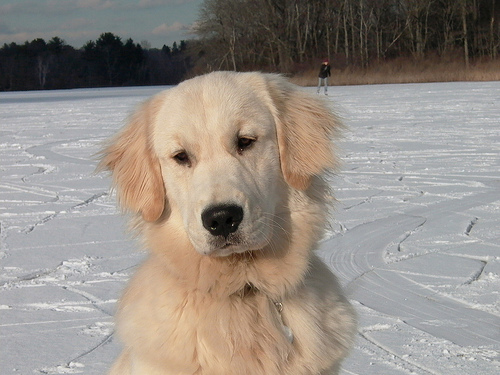
\includegraphics[width=0.235\textwidth,height=0.15\textheight,keepaspectratio]{dataset_examples/imagenet_val_golden_retriever.jpeg}}
        & \makebox[0.235\textwidth][c]{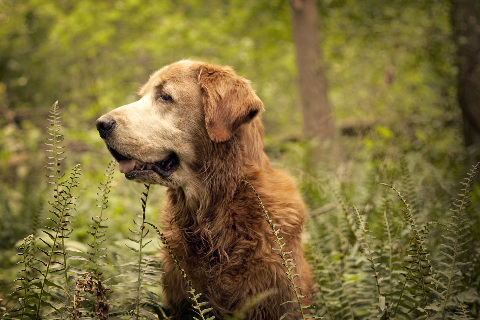
\includegraphics[width=0.235\textwidth,height=0.15\textheight,keepaspectratio]{dataset_examples/imagenet_v2_golden_retriever.jpeg}}
        & \makebox[0.235\textwidth][c]{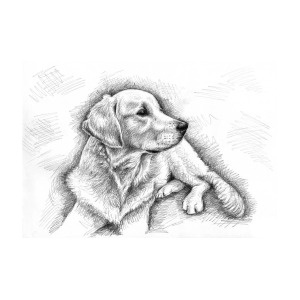
\includegraphics[width=0.235\textwidth,height=0.15\textheight,keepaspectratio]{dataset_examples/imagenet_sketch_golden_retriever.jpeg}} \\
        macaw
        & \makebox[0.235\textwidth][c]{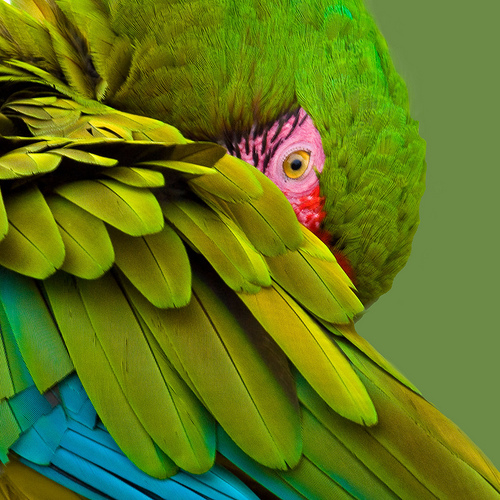
\includegraphics[width=0.235\textwidth,height=0.15\textheight,keepaspectratio]{dataset_examples/imagenet_val_macaw.jpeg}}
        & \makebox[0.235\textwidth][c]{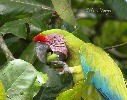
\includegraphics[width=0.235\textwidth,height=0.15\textheight,keepaspectratio]{dataset_examples/imagenet_v2_macaw.jpeg}}
        & \makebox[0.235\textwidth][c]{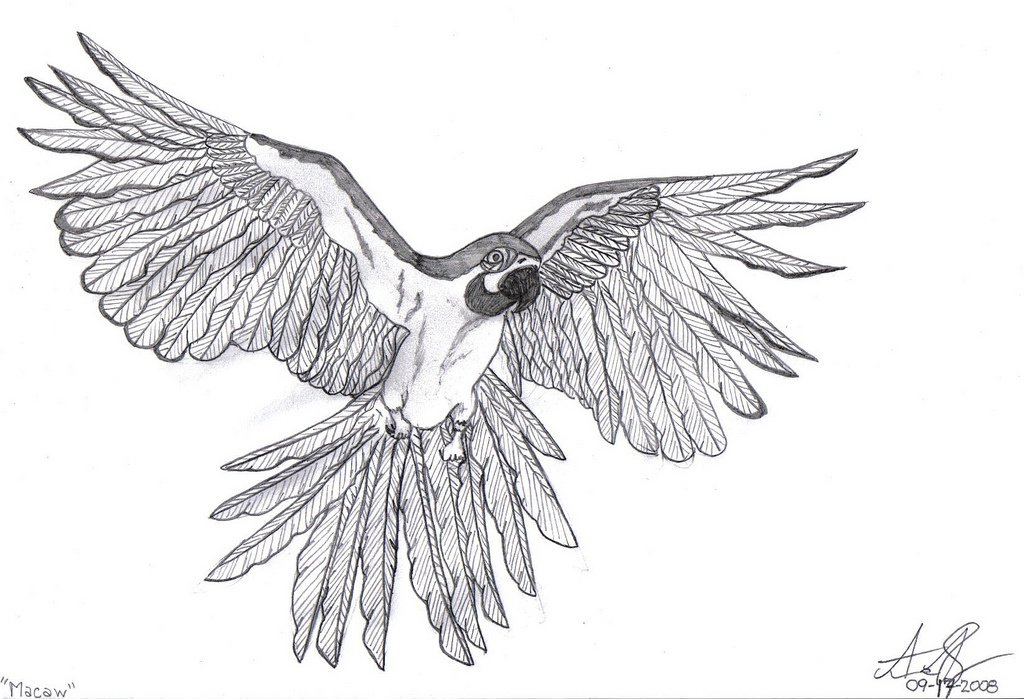
\includegraphics[width=0.235\textwidth,height=0.15\textheight,keepaspectratio]{dataset_examples/imagenet_sketch_macaw.jpeg}} \\
        strawberry
        & \makebox[0.235\textwidth][c]{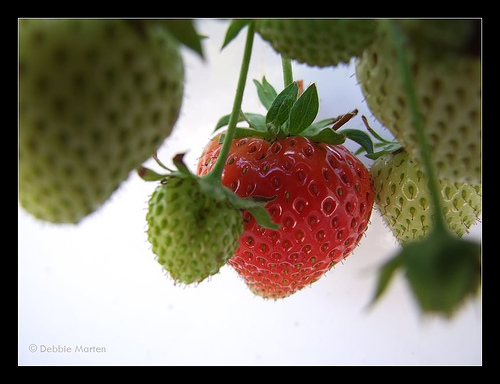
\includegraphics[width=0.235\textwidth,height=0.15\textheight,keepaspectratio]{dataset_examples/imagenet_val_strawberry.jpeg}}
        & \makebox[0.235\textwidth][c]{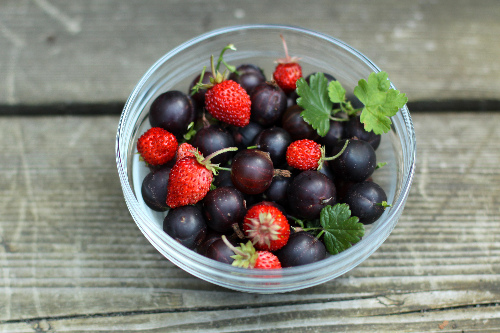
\includegraphics[width=0.235\textwidth,height=0.15\textheight,keepaspectratio]{dataset_examples/imagenet_v2_strawberry.jpeg}}
        & \makebox[0.235\textwidth][c]{
\includegraphics[width=0.235\textwidth,height=0.15\textheight,keepaspectratio]{dataset_examples/imagenet_sketch_strawberry.jpeg}} \\
    \end{tabular}
    \caption{Examples from the ImageNet-aligned shift ladder. Each row keeps the same class while changing the collection process or visual style.}
    \label{fig:dataset_shift_severity_ladder}
\end{figure}

\paragraph{Non-ImageNet domain checks.}
Chapter 8 also uses datasets whose visual domains are not ImageNet-like. ObjectNet contains household objects photographed under controlled variations in viewpoint, rotation, and background, and was designed to expose object-recognition brittleness outside standard ImageNet biases~\cite{barbu2019objectnet}. BloodMNIST and OrganAMNIST are part of MedMNIST v2, a lightweight benchmark suite for biomedical image classification~\cite{yang2023medmnist}: BloodMNIST contains RGB microscopy images of blood cells, while OrganAMNIST contains abdominal CT slices. RVL-CDIP contains scanned document pages labeled by document type~\cite{harley2015rvlcdip}. These domains test tokenizer behavior on microscopy, medical images, and document layouts. Table~\ref{tab:non_imagenet_datasets} summarizes the datasets, and Figure~\ref{fig:non_imagenet_domain_examples} shows representative inputs.

\begin{table}[htbp]
    \centering
    \scriptsize
    \renewcommand{\arraystretch}{1.15}
    \setlength{\tabcolsep}{3pt}
    \begin{tabularx}{\textwidth}{>{\raggedright\arraybackslash}p{0.14\textwidth} >{\raggedright\arraybackslash}X >{\raggedleft\arraybackslash}p{0.11\textwidth} >{\raggedright\arraybackslash}X}
        \textbf{Dataset} & \textbf{Content} & \textbf{Images used} & \textbf{Role in Chapter 8} \\ \hline
        ObjectNet & Controlled object photos with varied viewpoints and backgrounds & 50{,}273 & Natural-object domain with different pose and background statistics. \\
        BloodMNIST & Microscopic RGB blood-cell images, 8 classes & 17{,}092 & Biomedical microscopy, dominated by local texture and cellular morphology. \\
        OrganAMNIST & Abdominal CT slices, 11 organ classes & 57{,}187 & Grayscale medical imaging with intensity statistics far from natural images. \\
        RVL-CDIP & Scanned document pages, 16 document classes & 39{,}996 & Layout- and text-like structure rather than natural-image content. \\
    \end{tabularx}
    \caption{Non-ImageNet datasets used as domain-shift checks. The image counts report the subsets used in the tokenizer experiments; for example, RVL-CDIP contains 400{,}000 images in the full source dataset.}
    \label{tab:non_imagenet_datasets}
\end{table}

\begin{figure}[t]
    \centering
    \setlength{\tabcolsep}{4pt}
    \renewcommand{\arraystretch}{1.15}
    \begin{tabular}{c c c c}
        \textbf{ObjectNet} & \textbf{BloodMNIST} & \textbf{OrganAMNIST} & \textbf{RVL-CDIP} \\
        \makebox[0.22\textwidth][c]{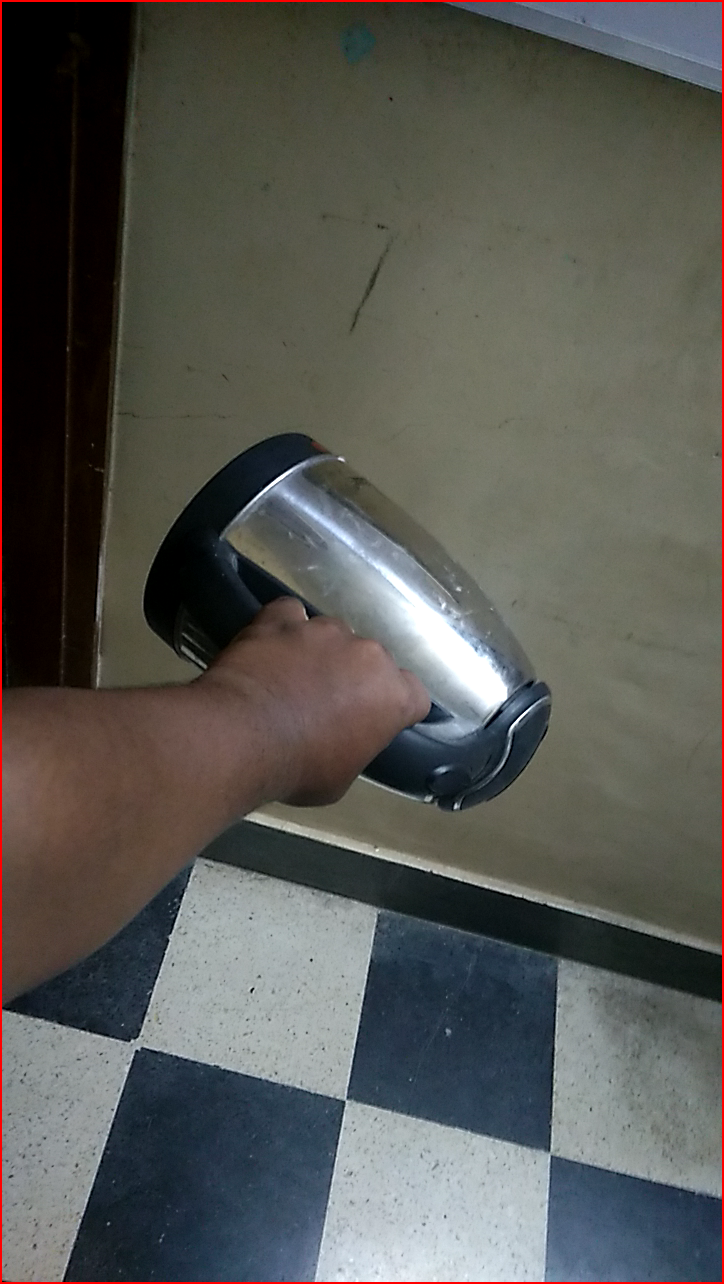
\includegraphics[width=0.16\textwidth,height=0.105\textheight,keepaspectratio]{dataset_examples/ood_objectnet_kettle.png}} &
        \makebox[0.22\textwidth][c]{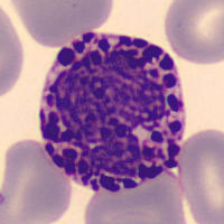
\includegraphics[width=0.16\textwidth,height=0.105\textheight,keepaspectratio]{dataset_examples/ood_bloodmnist_class0.png}} &
        \makebox[0.22\textwidth][c]{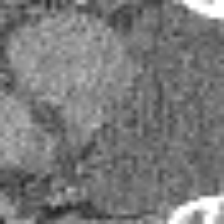
\includegraphics[width=0.16\textwidth,height=0.105\textheight,keepaspectratio]{dataset_examples/ood_organamnist_class0.png}} &
        \makebox[0.22\textwidth][c]{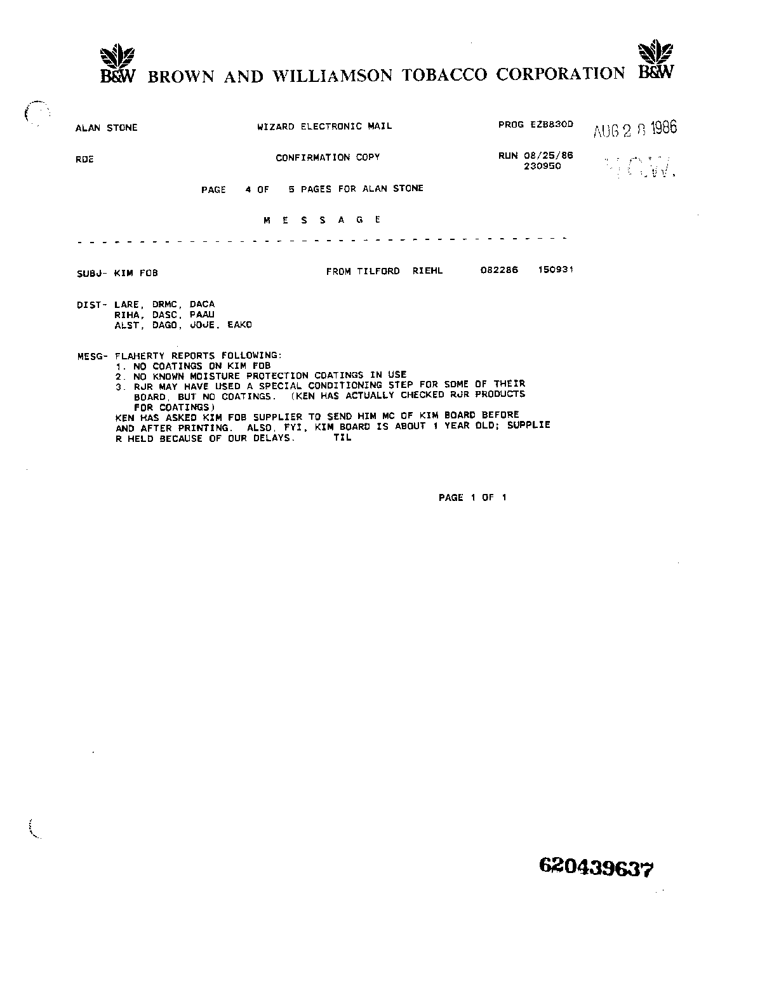
\includegraphics[width=0.16\textwidth,height=0.105\textheight,keepaspectratio]{dataset_examples/ood_rvlcdip_email.png}} \\
        kettle & class 0 & class 0 & email \\
        \makebox[0.22\textwidth][c]{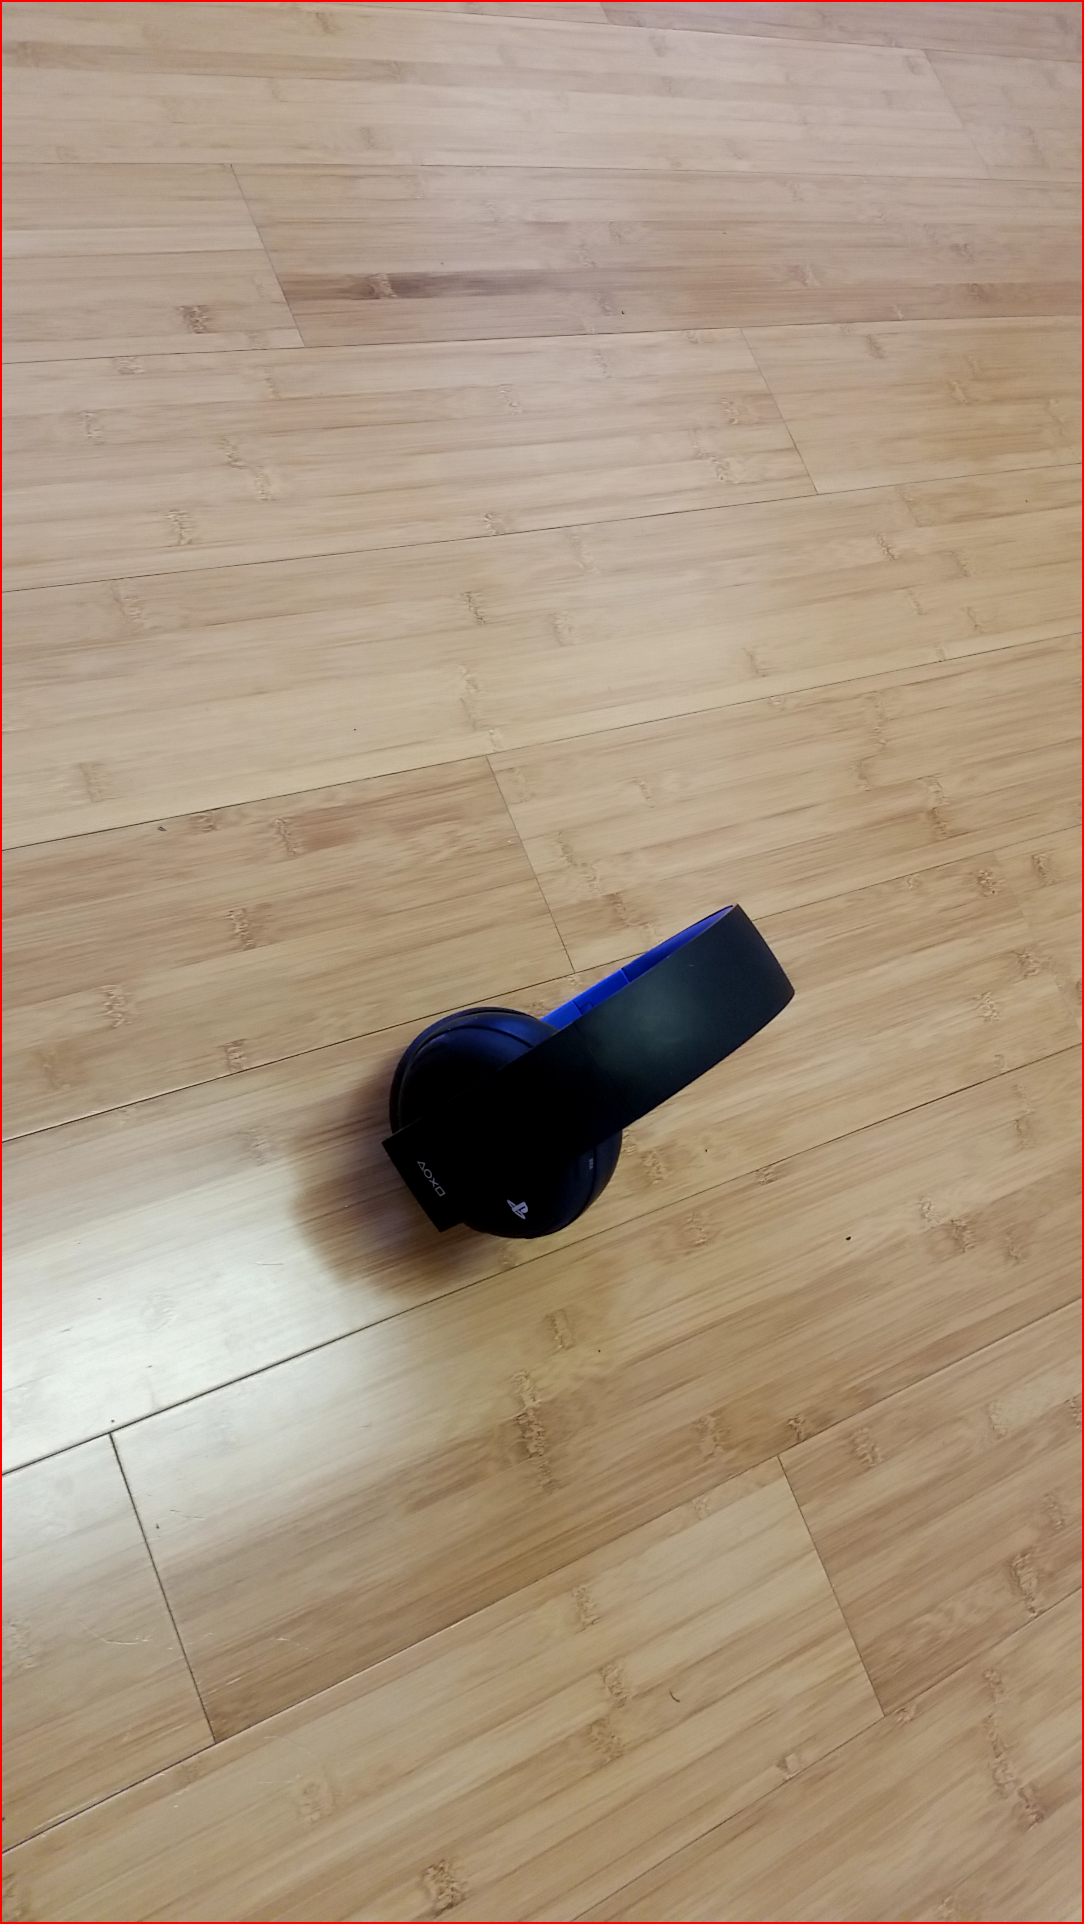
\includegraphics[width=0.16\textwidth,height=0.105\textheight,keepaspectratio]{dataset_examples/ood_objectnet_headphones.png}} &
        \makebox[0.22\textwidth][c]{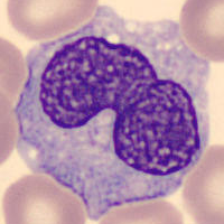
\includegraphics[width=0.16\textwidth,height=0.105\textheight,keepaspectratio]{dataset_examples/ood_bloodmnist_class5.png}} &
        \makebox[0.22\textwidth][c]{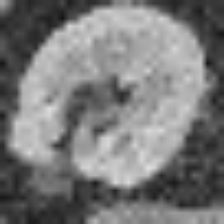
\includegraphics[width=0.16\textwidth,height=0.105\textheight,keepaspectratio]{dataset_examples/ood_organamnist_class5.png}} &
        \makebox[0.22\textwidth][c]{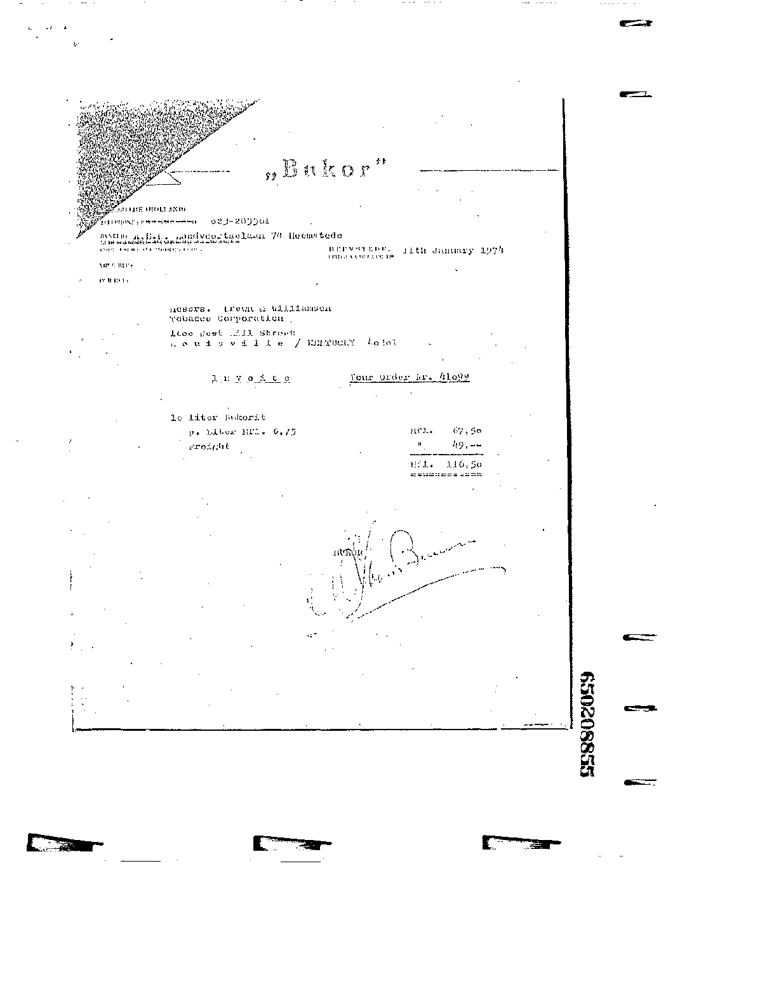
\includegraphics[width=0.16\textwidth,height=0.105\textheight,keepaspectratio]{dataset_examples/ood_rvlcdip_invoice.png}} \\
        headphones & class 5 & class 5 & invoice
    \end{tabular}
    \caption{Representative non-ImageNet domain examples. ObjectNet remains object-centric, while BloodMNIST, OrganAMNIST, and RVL-CDIP move to biomedical or document domains.}
    \label{fig:non_imagenet_domain_examples}
\end{figure}

\section{Metrics}
\label{sec:metrics}

A tokenizer can be evaluated by reconstruction quality, codebook usage, and its
response to perturbations. Token frequencies determine the distribution that
the autoregressive model must learn. Perturbation response can be measured by
how far changes spread through the token grid or decoded image.

We group the metrics by what they measure: paired-image reconstruction,
image-set distributions, codebook usage, and perturbation locality. Paired
metrics compare each reconstruction with its source image. Distribution metrics
compare the aggregate distributions of two image sets; FID and related metrics
perform this comparison in a particular learned feature space. Codebook metrics
measure which codes are used and how concentrated their frequencies are.
Perturbation metrics compare matched outputs before and after an intervention,
either globally or within specified spatial regions. Figure~\ref{fig:metric_taxonomy_matrix}
summarizes these four families.

\begin{figure}[t]
    \centering
    \begingroup
\scriptsize
\renewcommand{\arraystretch}{1.16}
\setlength{\tabcolsep}{3.5pt}
\begin{tabularx}{\textwidth}{>{\raggedright\arraybackslash}p{0.18\textwidth} >{\raggedright\arraybackslash}p{0.25\textwidth} >{\raggedright\arraybackslash}p{0.25\textwidth} >{\centering\arraybackslash}X}
\rowcolor{blue!9}
\textbf{Metric family} & \textbf{Quantities used} & \textbf{Comparison unit} & \textbf{Interpretation} \\ \hline
Paired-image reconstruction & PSNR, SSIM, LPIPS & One input $x$ and its reconstruction $\hat{x}$ & PSNR, SSIM $\uparrow$; LPIPS $\downarrow$ \\
Image-set distributions & FID, sFID, precision, recall, IS & Reference and reconstruction sets & distribution agreement; IS is diagnostic \\
Codebook usage & Active codes, entropy, perplexity, top-$m$ mass & All token assignments in an evaluation set & descriptive, not a quality score \\
Perturbation locality & Flip rate, inside/outside response, leakage ratio & Matched outputs and spatial regions & less outside response means greater locality \\
\end{tabularx}
\endgroup

    \caption{Metric taxonomy used in this thesis. Evaluation combines sample-level reconstruction metrics, distribution-level image metrics, codebook-usage measures, and locality-oriented measures.}
    \label{fig:metric_taxonomy_matrix}
\end{figure}

\subsection{Sample-Level Reconstruction Metrics}
\label{subsec:sample_reconstruction_metrics}

Full-reference metrics compare each reconstruction with its corresponding
original image. Mean squared error (MSE) and peak signal-to-noise ratio (PSNR)
are full-reference pixel metrics. For an image with $N$ scalar pixel values,
\begin{align}
    \mathrm{MSE}(x,\hat{x}) &= \frac{1}{N}\sum_{i=1}^{N}(x_i-\hat{x}_i)^2, \\
    \mathrm{PSNR}(x,\hat{x}) &= 10\log_{10}\!\left(\frac{\mathrm{MAX}^2}{\mathrm{MSE}(x,\hat{x})}\right).
\end{align}
For normalized images in $[0,1]$, $\mathrm{MAX}=1$. Lower MSE and higher PSNR indicate better pixel agreement. PSNR is widely used in image restoration but is known to be limited as a perceptual quality measure~\cite{huynh2008scope}.

SSIM compares local luminance, contrast, and structure rather than only pointwise pixel error~\cite{wang2004ssim}. In simplified form,
\begin{equation}
    \mathrm{SSIM}(x,y) = l(x,y)c(x,y)s(x,y),
\end{equation}
where $l$, $c$, and $s$ denote luminance, contrast, and structure comparisons computed over local windows. SSIM values are then averaged across the image. Higher SSIM indicates stronger structural similarity.

LPIPS compares normalized deep-network activations between two images~\cite{zhang2018unreasonable}:
\begin{equation}
    \mathrm{LPIPS}(x,y)
    = \sum_l \frac{1}{H_lW_l}\sum_{h,w}
    \left\lVert
    w_l \odot \left(\hat\phi_l(x)_{h,w}-\hat\phi_l(y)_{h,w}\right)
    \right\rVert_2^2,
\end{equation}
where $\hat\phi_l$ denotes channel-normalized features at layer $l$, $w_l$
contains learned channel weights, and the distance is averaged over the
$H_l\times W_l$ spatial locations. Lower LPIPS indicates greater perceptual
similarity. Unlike MSE and PSNR, LPIPS is calibrated against human perceptual
judgments. The reconstruction evaluator used here uses its VGG-16 backbone.

\subsection{Distribution-Level Image Metrics}
\label{subsec:distribution_metrics}

FID compares two image sets by embedding them with an Inception network and fitting a Gaussian to each feature distribution~\cite{heusel2017gans}. For reference features with mean and covariance $(\mu_r,\Sigma_r)$ and reconstruction features with $(\mu_g,\Sigma_g)$,
\begin{equation}
    \mathrm{FID}
    =
    \lVert \mu_r-\mu_g\rVert_2^2
    +
    \mathrm{Tr}\!\left(\Sigma_r+\Sigma_g-2(\Sigma_r\Sigma_g)^{1/2}\right).
\end{equation}
Lower FID indicates closer feature distributions. In the literature on VQ
tokenizers, VQGAN and LlamaGen report reconstruction FID or rFID to compare the
distribution of reconstructions with original images
~\cite{esser2021taming,sun2024llamagen}.

sFID is a spatial variant used in common diffusion-model evaluator pipelines~\cite{dhariwal2021diffusion,openaiguideddiffusion,openaiguideddiffusionevals}. It uses spatial features rather than only pooled Inception features, so it can be more sensitive to spatial layout differences. It carries the same finite-sample and feature-extractor caveats as FID.

Inception Score uses an Inception classifier~\cite{salimans2016improved}:
\begin{equation}
    \mathrm{IS}
    =
    \exp\!\left(
        \mathbb{E}_{x\sim p_g}
        \left[
            \mathrm{KL}\!\left(p(y\mid x)\,\|\,p(y)\right)
        \right]
    \right).
\end{equation}
Here, $p(y\mid x)$ is the classifier's conditional class distribution for one
reconstruction and $p(y)$ is the marginal class distribution across the set.
The score increases when individual predictions are confident and predictions
across the set cover different classes. It does not measure whether a
reconstruction matches its input, so we report it as a classifier-based
diagnostic~\cite{barratt2018note,chong2019unbiased}.

For reconstructed image sets, precision measures how much of the reconstruction
distribution lies near the reference feature distribution, while recall
measures how much of the reference distribution is covered
~\cite{kynkaanniemi2019improved}. Figure~\ref{fig:precision_recall_tradeoff}
illustrates this distinction.

\begin{figure}[t]
    \centering
    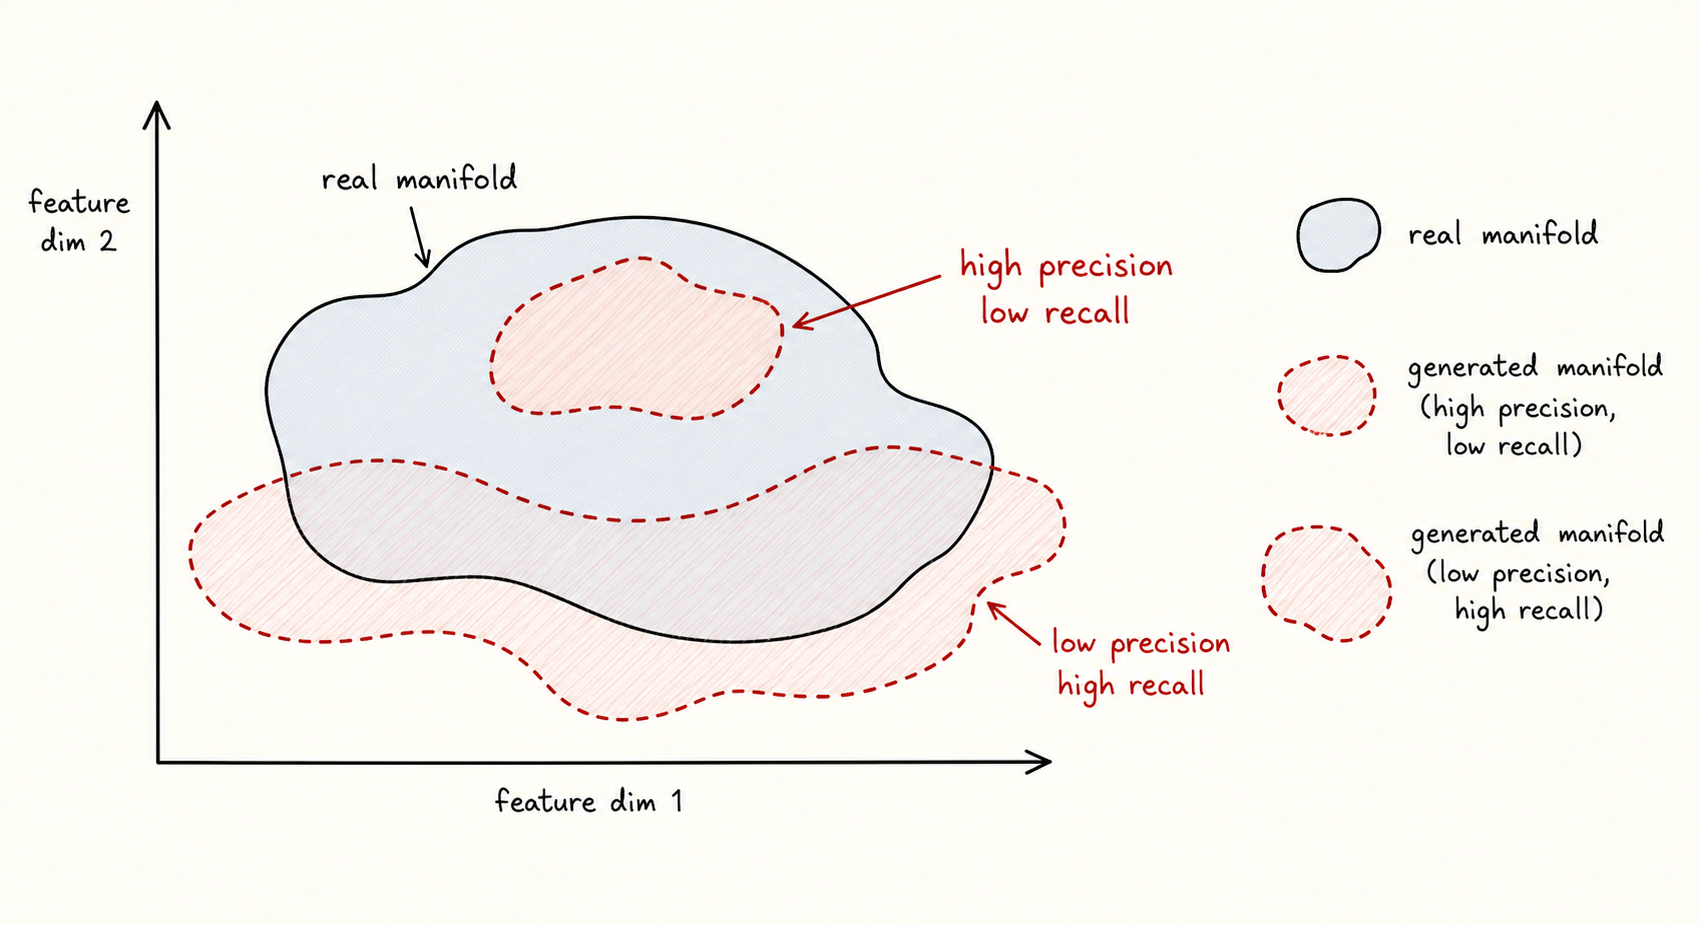
\includegraphics[width=0.9\textwidth]{ch03_fig_3_3_precision_recall_tradeoff.png}
    \caption{Fidelity and coverage manifolds for Precision and Recall. Precision measures the portion of generated support within the real data manifold; Recall measures coverage of the real manifold. Source: reproduced from Kynk\"a\"anniemi et al.~\cite{kynkaanniemi2019improved}.}
    \label{fig:precision_recall_tradeoff}
\end{figure}

\subsection{Codebook Usage Metrics}
\label{subsec:codebook_usage_metrics}

Let $n_k$ be the number of assignments to code $k$ over an evaluation set, let $N_t=\sum_{k=1}^{K}n_k$ be the total number of token assignments, and let
\begin{equation}
    p_k = \frac{n_k}{N_t}.
\end{equation}
$p_k$ is the fraction of all observed token assignments that use code $k$.
The raw active-code count is
\begin{equation}
    A_{\mathrm{raw}} = \sum_{k=1}^{K}\mathbf{1}[n_k>0],
\end{equation}
and the active fraction is
\begin{equation}
    a_{\mathrm{raw}} = \frac{A_{\mathrm{raw}}}{K}.
\end{equation}
The active-code count is the number of distinct codes used at least once;
dividing it by $K$ gives the active fraction. Because a single assignment makes
a code active under this definition, Chapter~\ref{ch:rq1} also reports two
support measures. The effective active set counts codes with
$p_k\geq10^{-6}$, which is at least 13 of the 12.8 million assignments in that
evaluation. The cumulative support $C_{99}$ is the smallest frequency-ranked
set of codes covering 99\% of assignments. These measures are distinct from
perplexity, which summarizes the full frequency distribution.

Entropy and perplexity summarize how spread out the token distribution is:
\begin{align}
    H(p) &= -\sum_{k=1}^{K} p_k\log p_k, \\
    P(p) &= \exp(H(p)).
\end{align}
The intuitive meaning of perplexity is effective vocabulary size. If the tokenizer used exactly $M$ codes uniformly, then $P(p)=M$. A tokenizer may therefore have $K=16{,}384$ nominal entries but a much smaller effective vocabulary if the distribution is concentrated.

Top-$m$ mass measures concentration directly:
\begin{equation}
    M_m = \sum_{k\in \mathrm{Top}_m(p)} p_k,
\end{equation}
where $\mathrm{Top}_m(p)$ is the set of the $m$ most frequent codes. High top-$m$ mass means that a small set of codes accounts for a large fraction of assignments.

Finally, positional entropy computes the same entropy quantity at each grid position $(u,v)$ across the dataset. It asks whether different spatial positions use similar parts of the codebook or whether some positions specialize to particular tokens.

\subsection{Locality and Robustness Metrics}
\label{subsec:locality_robustness_metrics}

Perturbation metrics compare tokenizer outputs before and after a controlled
change. A global response can be measured as the change in reconstruction or
codebook statistics. Spatial locality uses a mask to divide the response into
inside and outside regions. For token position $i$, define a flip indicator
\begin{equation}
    F_i = \mathbf{1}[t_i \ne t'_i],
\end{equation}
where $t_i$ and $t'_i$ are the clean and perturbed token assignments. For a set of token positions $R$,
\begin{equation}
    r(R) = \mathbb{E}_{i\in R}[F_i].
\end{equation}
For a local image perturbation, the leakage ratio compares outside-region and
inside-region flip rates:
\begin{equation}
    \lambda_{\mathrm{enc}} =
    \frac{r(R_{\mathrm{out}})}
         {r(R_{\mathrm{in}})+\varepsilon}.
\end{equation}
The small constant $\varepsilon$ avoids division by zero when no inside-patch flips occur. A low leakage ratio means that token changes are mostly confined to the perturbed region; a high value means that the encoder or quantizer has propagated the perturbation to distant token positions.

The same definition applies to decoder locality after replacing the token flip
indicator with an image-change measure. Later chapters specify the perturbation,
mask, and response measure used by each experiment.

\begin{figure}[t]
    \centering
    \resizebox{0.9\textwidth}{!}{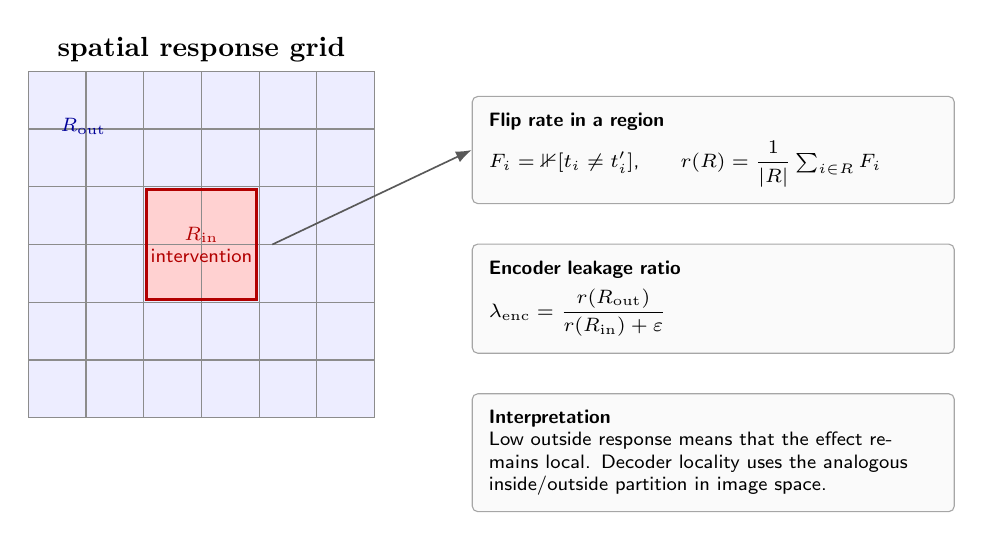
\begin{tikzpicture}[
    font=\sffamily\scriptsize,
    arrow/.style={-{Latex[length=2mm]}, semithick, black!65},
    eq/.style={draw=black!35, rounded corners=2pt, fill=black!2,
               text width=57mm, align=left, inner sep=6pt}
]
\begin{scope}[xshift=-58mm,yshift=-19mm]
    \fill[blue!7] (0,0) rectangle (44mm,44mm);
    \fill[red!18] (15mm,15mm) rectangle (29mm,29mm);
    \draw[step=7.333mm, black!45] (0,0) grid (44mm,44mm);
    \draw[red!70!black, very thick] (15mm,15mm) rectangle (29mm,29mm);
    \node[font=\bfseries, above] at (22mm,44mm) {spatial response grid};
    \node[red!70!black, align=center] at (22mm,22mm) {$R_{\mathrm{in}}$\\intervention};
    \node[blue!60!black, align=center] at (7mm,37mm) {$R_{\mathrm{out}}$};
\end{scope}

\node[eq] (flip) at (29mm,15mm)
    {\textbf{Flip rate in a region}\\[1mm]
     $F_i=\mathbb{1}[t_i\neq t_i']$,\qquad
     $r(R)=\dfrac{1}{|R|}\sum_{i\in R}F_i$};
\node[eq, below=5mm of flip] (leak)
    {\textbf{Encoder leakage ratio}\\[1mm]
     $\lambda_{\mathrm{enc}}=
     \dfrac{r(R_{\mathrm{out}})}{r(R_{\mathrm{in}})+\varepsilon}$};
\node[eq, below=5mm of leak] (interpret)
    {\textbf{Interpretation}\\Low outside response means that the effect remains local.
     Decoder locality uses the analogous inside/outside partition in image space.};
\draw[arrow] (-27mm,3mm) -- (flip.west);
\end{tikzpicture}
}
    \caption{Locality and leakage as measured in this thesis. Encoder locality compares clean and perturbed token assignments inside and outside the image patch mapped to token space. Decoder locality uses the analogous partition of the decoded image response.}
    \label{fig:locality_leakage_curve}
\end{figure}

\subsection{Metric Comparison Summary}
\label{subsec:metric_comparison_summary}

Table~\ref{tab:metric_comparison_summary} summarizes the metrics used in the
thesis. Paired metrics compare images, distribution metrics compare image sets,
codebook metrics describe token frequencies, and locality metrics describe the
response to controlled perturbations.

\begin{table}[t]
    \centering
    \scriptsize
    \renewcommand{\arraystretch}{1.18}
    \setlength{\tabcolsep}{3pt}
    \begin{tabularx}{\textwidth}{>{\raggedright\arraybackslash}p{0.12\textwidth} >{\raggedright\arraybackslash}p{0.20\textwidth} >{\raggedright\arraybackslash}p{0.18\textwidth} >{\raggedright\arraybackslash}p{0.17\textwidth} >{\raggedright\arraybackslash}X}
        \textbf{Metric} & \textbf{What it measures} & \textbf{Level} & \textbf{Direction} & \textbf{Main caveat} \\ \hline
        MSE / PSNR & Aligned pixel error & Sample image pair & MSE $\downarrow$, PSNR $\uparrow$ & Poor proxy for perceptual similarity. \\
        SSIM & Local luminance, contrast, and structure & Sample image pair & $\uparrow$ & Sensitive to alignment and window choices. \\
        LPIPS & Deep-feature perceptual distance & Sample image pair & $\downarrow$ & Depends on backbone and calibration. \\
        FID / sFID & Feature-distribution match between image sets & Image set & $\downarrow$ & Feature extractor, finite-sample, and Gaussian-assumption effects. \\
        IS & Classifier confidence and predicted-class diversity & Image set & $\uparrow$ & Does not directly compare outputs to real images. \\
        Precision / Recall & Fidelity to and coverage of a reference feature manifold & Image set & both $\uparrow$ & Depends on feature space and neighborhood construction. \\
        Active count / fraction & How much of the nominal codebook appears & Token distribution & $\uparrow$ & Raw activity is sensitive to rare one-off codes. \\
        Entropy / Perplexity & Effective spread of code usage & Token distribution & $\uparrow$ & Can hide spatial specialization. \\
        Top-$m$ mass & Concentration in frequent codes & Token distribution & $\downarrow$ & Choice of $m$ must be reported. \\
        Flip rate / leakage ratio & Token or image changes under controlled perturbation & Perturbation response & $\downarrow$ & Depends on perturbation mask and region definition. \\
    \end{tabularx}
    \caption{Compact comparison of metric families used in the thesis. Arrows indicate the preferred direction under a fixed evaluation protocol.}
    \label{tab:metric_comparison_summary}
\end{table}

\chapter{Reconstruction Baseline and Codebook Usage}
\label{ch:rq1}

Before any perturbation is introduced, this chapter establishes the clean
ImageNet baseline for the two studied tokenizers. It measures how well each
tokenizer reconstructs unmodified validation images and which empirical token
distribution it produces. Both tokenizers have the same nominal vocabulary
size, $K=16{,}384$, and produce a $16\times16$ token grid from a
$256\times256$ image, making their outputs directly comparable.

\section{Experimental Setup}
\label{sec:rq1_experimental_setup}

For each image $x$, the tokenizer produces a reconstruction:

\begin{equation}
\hat{x} = D(Q(E(x))),
\end{equation}

where $E$ is the encoder, $Q$ is the vector-quantization step, and $D$ is the decoder. Reconstruction quality is measured using the metrics defined in Chapter~\ref{ch:datasets_models_metrics}: PSNR, SSIM, LPIPS, FID, sFID, precision, recall, and Inception Score. Codebook usage is computed from the discrete token grids over all 50,000 validation images. Since each image produces a $16 \times 16$ grid, each tokenizer contributes:

\begin{equation}
50{,}000 \times 16 \times 16 = 12{,}800{,}000
\end{equation}

token assignments for the ImageNet baseline.

The codebook analysis reports both raw and effective vocabulary use. The raw active count is the number of codebook entries assigned at least once. The effective active count uses a minimum-frequency threshold of $10^{-6}$ of all token assignments, corresponding to at least 13 assignments out of 12.8 million tokens in this experiment. Entropy and perplexity summarize the effective size of the empirical distribution, and top-$k$ mass measures how much of the token stream is captured by the most frequent codes.

The experiment uses the same ImageNet validation images and deterministic
inference for both models. Each exporter applies its own resize filter before
the $256\times256$ center crop; Appendix~\ref{app:computational_environment}
documents this preprocessing difference.

\section{Reconstruction Baseline}
\label{sec:rq1_reconstruction_baseline}

Table~\ref{tab:rq1_reconstruction_metrics} reports the ImageNet reconstruction metrics for LlamaGen and VQGAN. LlamaGen improves the paired-image metrics (PSNR, SSIM, LPIPS) and the reference-conditioned distribution metrics (FID, sFID, precision, and recall). Inception Score is retained as a diagnostic of classifier confidence and class diversity, not treated as a paired reconstruction metric or as having a universally preferred direction. The remaining metrics make LlamaGen the stronger clean reconstruction baseline on ImageNet.

\begin{table}[t]
    \centering
    \small
    \setlength{\tabcolsep}{4pt}
    \begin{tabular}{lrrrrrrrr}
        \textbf{Tokenizer} & \textbf{PSNR} & \textbf{SSIM} & \textbf{LPIPS} & \textbf{FID} & \textbf{sFID} & \textbf{Precision} & \textbf{Recall} & \textbf{IS} \\ \hline
        LlamaGen & 20.79 & 0.558 & 0.228 & 2.19 & 5.01 & 0.978 & 0.995 & 52.70 \\
        VQGAN    & 19.65 & 0.489 & 0.286 & 5.06 & 6.49 & 0.920 & 0.973 & 46.76 \\
    \end{tabular}
    \caption{ImageNet reconstruction metrics for the two tokenizers. Higher PSNR, SSIM, precision, and recall are preferred; lower LPIPS, FID, and sFID are preferred. Inception Score is reported as a diagnostic and is not assigned a preferred reconstruction direction.}
    \label{tab:rq1_reconstruction_metrics}
\end{table}

The PSNR gap is modest in absolute terms, but it is consistent with the other metrics. LlamaGen reaches a mean PSNR of 20.79 compared with 19.65 for VQGAN, and a mean SSIM of 0.558 compared with 0.489. LPIPS also favors LlamaGen: 0.228 compared with 0.286 for VQGAN. Because LPIPS is computed in a learned feature space, the reconstruction difference extends beyond pixel-level measurements. The distributional metrics agree with the same direction: LlamaGen obtains FID 2.19 and sFID 5.01, while VQGAN obtains FID 5.06 and sFID 6.49.

The corresponding per-image standard deviations are 3.18 dB, 0.167, and
0.058 for LlamaGen PSNR, SSIM, and LPIPS, and 3.41 dB, 0.176, and 0.066 for
VQGAN. These standard deviations describe variation across images, not
uncertainty in the dataset means or the fraction of images on which one model
wins. FID and related distribution metrics do
not decompose into per-image observations and are consequently reported as
dataset-level estimates.

The published LlamaGen comparison reports PSNR $20.79$, SSIM $0.675$, and
reconstruction FID $2.19$ for VQ-16, versus PSNR $20.00$, SSIM $0.629$, and
FID $4.99$ for VQGAN-f16-16384~\cite{sun2024llamagen}. Our LlamaGen PSNR and
FID agree to the displayed precision. The SSIM values are not directly
comparable. The public LlamaGen evaluation script sets the SSIM data range to
$2.0$ for images in $[0,1]$, whereas our exporters set it to $1.0$ and use
scikit-image's default window with the last axis as the color channel. Our
VQGAN PSNR and FID also differ from the published values;
the resize filters differ between exporters, so these numbers do not establish
the cause of that offset. LlamaGen's published $97\%$ usage is measured in a
65{,}536-token queue, whereas our $100\%$ denotes codes observed at least once
across 12.8 million assignments.

Figure~\ref{fig:rq1_reconstruction_metric_comparison} visualizes the same comparison across metrics that differ in scale and direction. Excluding Inception Score, whose interpretation is not paired to a reference image, the reconstruction metrics consistently favor LlamaGen.

\begin{figure}[t]
    \centering
    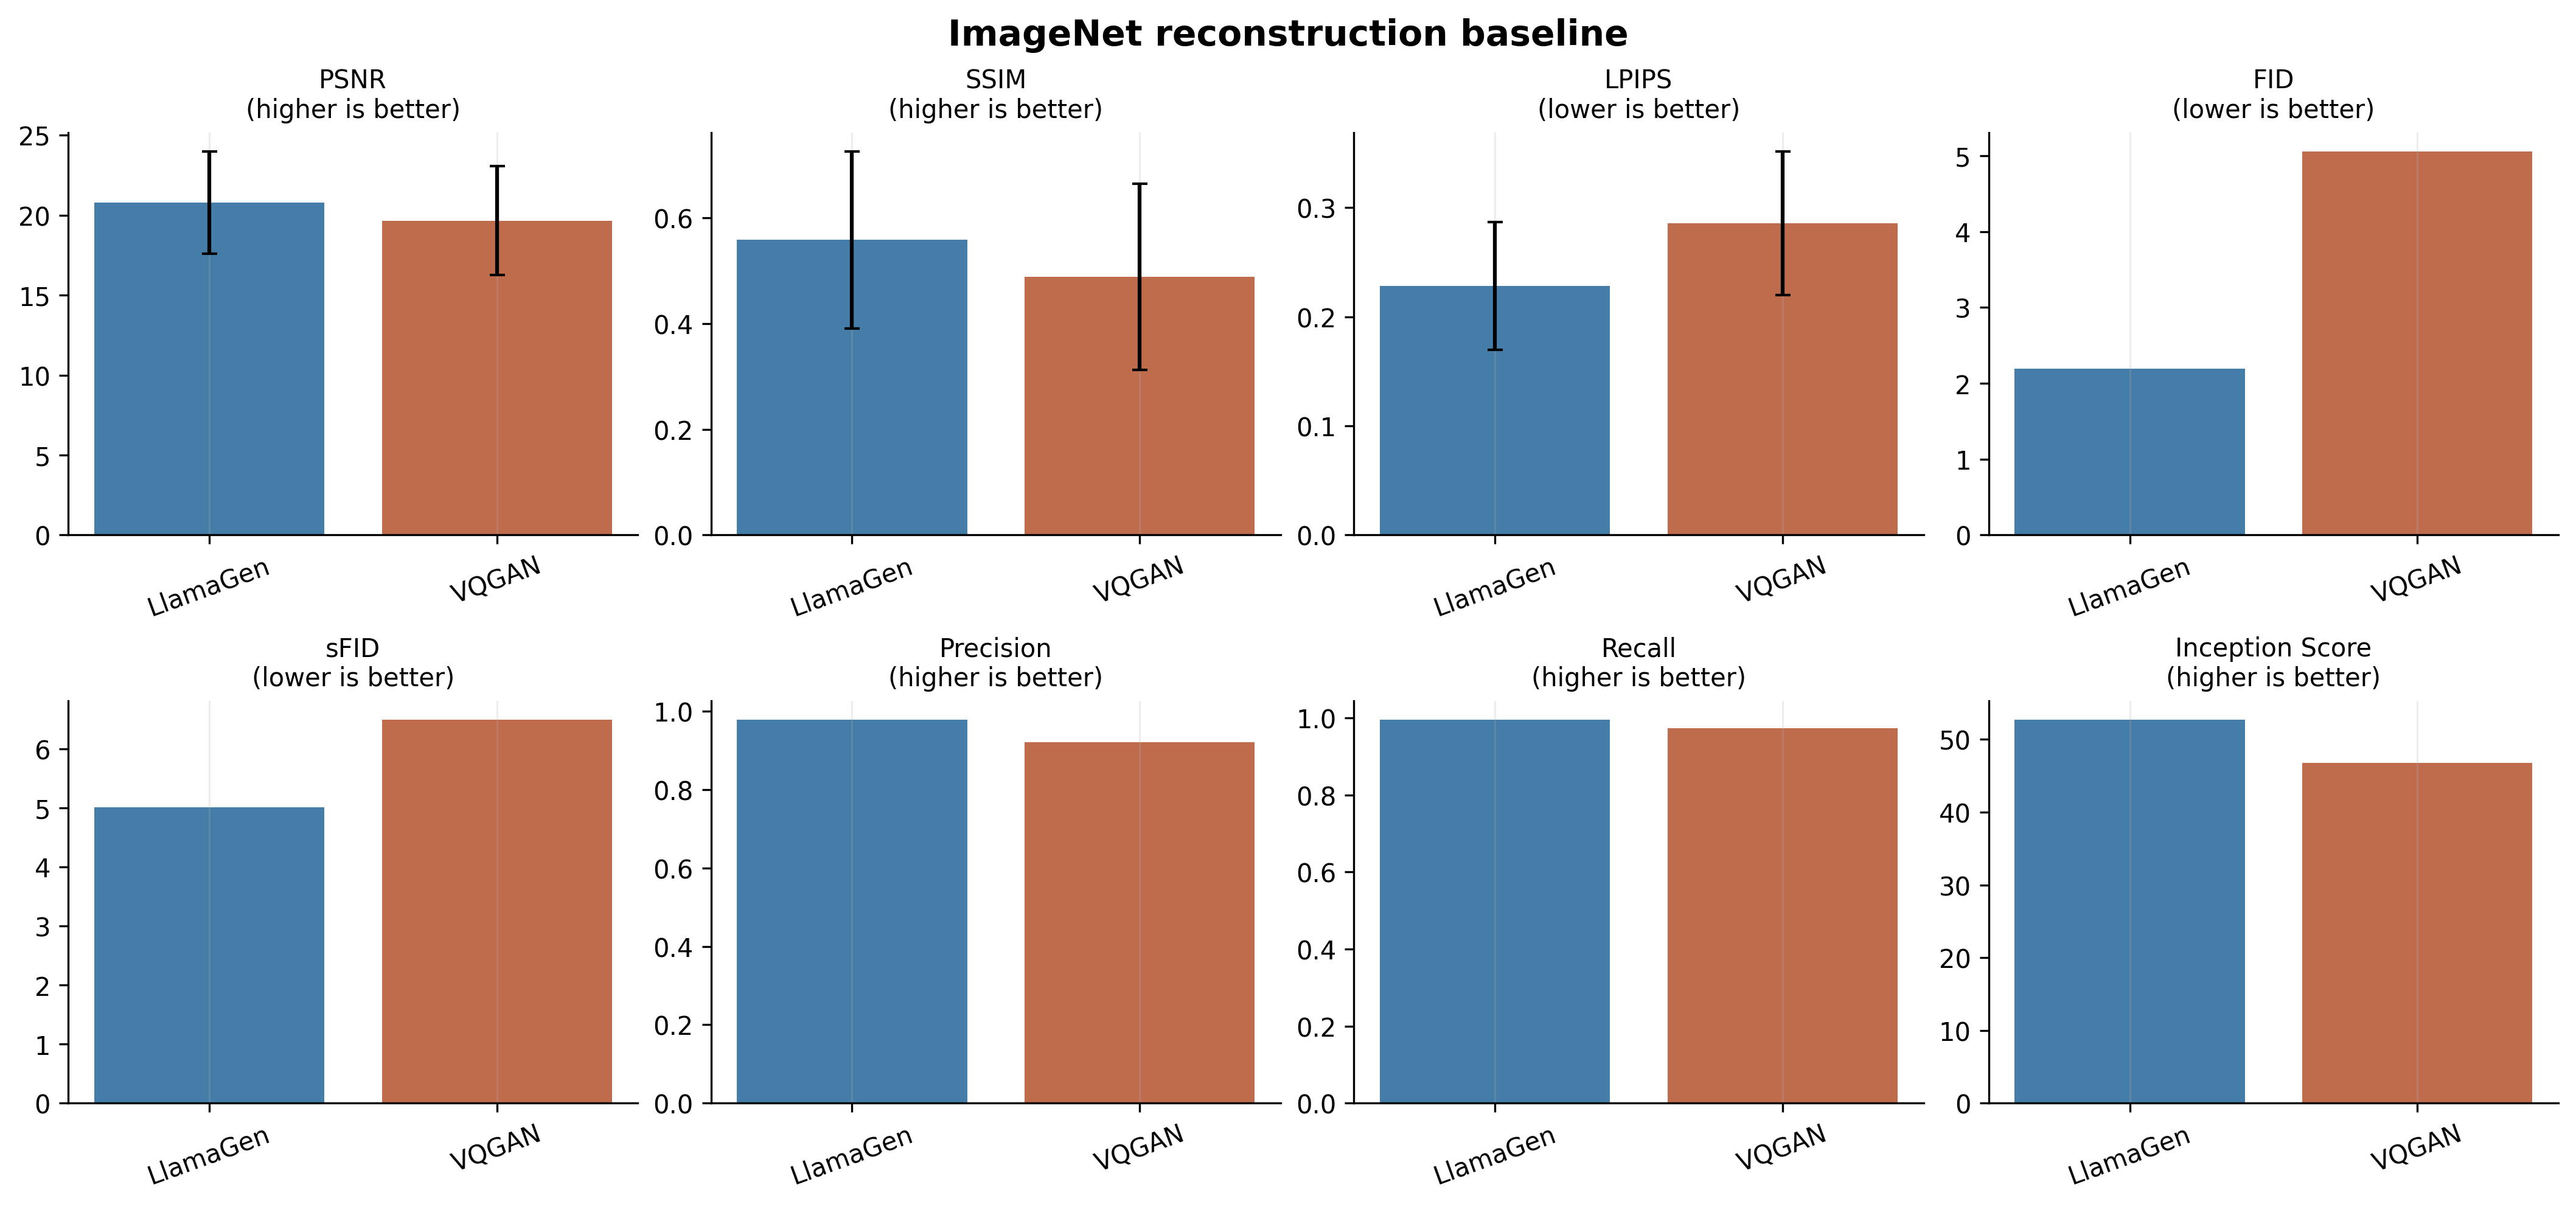
\includegraphics[width=0.98\textwidth]{ch04_fig_reconstruction_metric_comparison.png}
    \caption{ImageNet reconstruction metric comparison for VQGAN and LlamaGen. Each panel names whether higher or lower values are preferred; the comparison should be read by direction within each metric, not by comparing bar heights across panels.}
    \label{fig:rq1_reconstruction_metric_comparison}
\end{figure}

Figure~\ref{fig:rq1_reconstruction_triplets} shows how much detail and structure
each tokenizer preserves through the discrete bottleneck on three paired
examples.

\begin{figure}[t]
    \centering
    
\includegraphics[width=0.9\textwidth]{ch04_fig_reconstruction_triplets.png}
    \caption{Qualitative ImageNet reconstruction examples. Each row shows the original image, the VQGAN reconstruction, and the LlamaGen reconstruction.}
    \label{fig:rq1_reconstruction_triplets}
\end{figure}

\section{Codebook Usage}
\label{sec:rq1_codebook_usage}

The metrics above show that LlamaGen reconstructs the ImageNet validation images more accurately than VQGAN under the recorded exporter settings. The following analysis examines whether the two tokenizers also differ in how they use their discrete vocabularies. Table~\ref{tab:rq1_codebook_usage} reports the main usage statistics.

\begin{table}[t]
    \centering
    \small
    \setlength{\tabcolsep}{4pt}
    \resizebox{\textwidth}{!}{%
    \begin{tabular}{lrrrrrrr}
        \textbf{Tokenizer} & \textbf{Codebook size} & \textbf{Active} & \textbf{Effective active} & \textbf{Perplexity} & \textbf{Top-10} & \textbf{Top-100} & \textbf{Top-500} \\ \hline
        LlamaGen & 16{,}384 & 16{,}384 (100.0\%) & 16{,}384 (100.0\%) & 16{,}179.19 & 0.003 & 0.012 & 0.046 \\
        VQGAN    & 16{,}384 & 972 (5.9\%)       & 971 (5.9\%)       & 910.46    & 0.022 & 0.165 & 0.665 \\
    \end{tabular}
    }
    \caption{ImageNet codebook usage summary. Active counts report how many nominal codes appear on ImageNet; effective active counts use the threshold of at least 13 assignments. Top-$k$ values report the fraction of all token assignments covered by the most frequent $k$ codes.}
    \label{tab:rq1_codebook_usage}
\end{table}

LlamaGen uses all 16,384 codebook entries on ImageNet with a perplexity of 16,179. This means that the empirical token distribution is close to uniform over the full nominal vocabulary. VQGAN uses only 972 of 16,384 codes, or about 5.9\% of the nominal codebook. Liu et al.~\cite{liu2024elucidating} previously reported approximately 1{,}000 used codes for this released VQGAN checkpoint on ImageNet training data; our validation-set count confirms that underuse under a different sample and protocol. Its perplexity of 910 is close to the raw active count, so the active subset is small but not dominated by only a handful of codes.

LlamaGen's top-500 codes account for only 4.6\% of all token assignments; VQGAN's top-500 account for 66.5\%. Thus, although the two tokenizers expose the same nominal vocabulary size, the sequences they would provide to a downstream autoregressive model have very different empirical vocabularies. The downstream model is trained on this empirical token stream, not on the unused portion of the nominal codebook.

Entropy gives an idealized coding interpretation of the same result. Since
$H=\log(\operatorname{PPL})$, the observed perplexities correspond to about
$9.69$ nats ($13.98$ bits) per token for LlamaGen and $6.81$ nats ($9.83$
bits) per token for VQGAN. For a 256-token grid, these are approximately
$3{,}579$ and $2{,}516$ idealized bits per image under an optimal code matched
to each empirical marginal distribution. LlamaGen's empirical marginal
entropy is therefore about 42\% higher. These marginal entropies describe ideal
code lengths for the observed token frequencies. They do not measure semantic
content or the conditional code length of a trained autoregressive model.

Figure~\ref{fig:rq1_code_usage_sorted} shows the full rank-frequency curve. LlamaGen assigns probability mass across the full codebook. VQGAN has a shorter curve because most nominal codes are inactive on ImageNet, and its active codes carry substantially higher average frequency.

\begin{figure}[t]
    \centering
    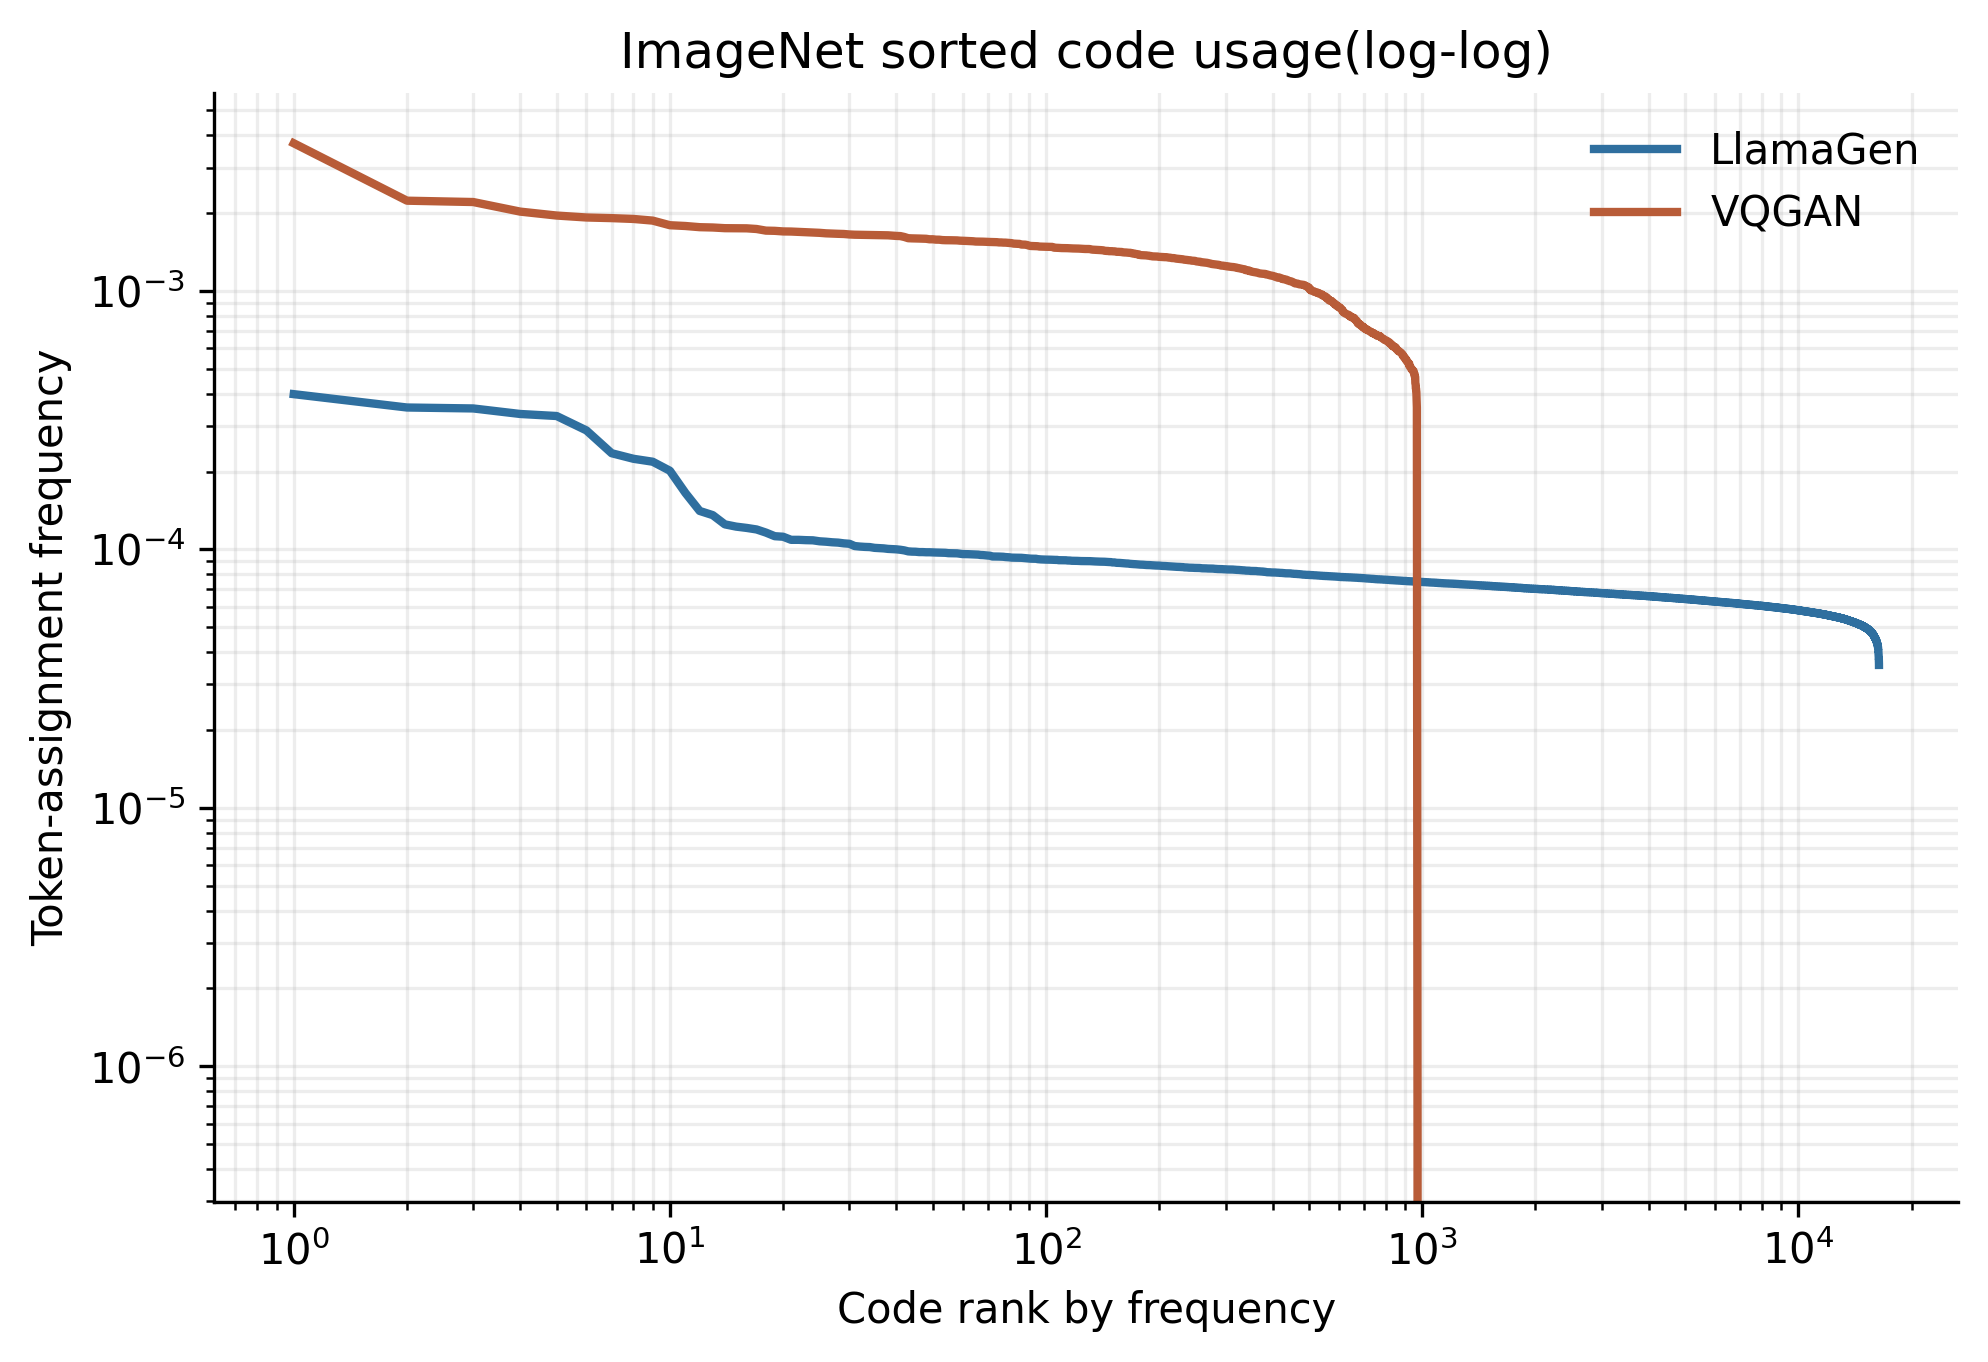
\includegraphics[width=0.78\textwidth]{ch04_fig_code_usage_sorted.png}
    \caption{Sorted ImageNet code-usage distribution. Codes are ranked by empirical frequency. The VQGAN curve ends near rank 972 because the remaining nominal codes are inactive on ImageNet.}
    \label{fig:rq1_code_usage_sorted}
\end{figure}

The top-$k$ columns in Table~\ref{tab:rq1_codebook_usage} report the cumulative
mass of the 10, 100, and 500 most frequent codes. High top-$k$ mass means that a
large fraction of the token sequence comes from a small set of IDs.

\section{Baseline Summary}
\label{sec:rq1_joint_view}

The baseline has two parts. First, LlamaGen gives better clean ImageNet reconstructions under the reported sample-level and distribution-level metrics. Second, the two tokenizers use their nominally equal codebooks very differently. Table~\ref{tab:rq1_joint_summary} keeps a compact version of these two facts together.

\begin{table}[t]
    \centering
    \scriptsize
    \begin{tabular}{lrrrrrrrr}
        \textbf{Tokenizer} & \textbf{PSNR} & \textbf{SSIM} & \textbf{LPIPS} & \textbf{FID} & \textbf{Active} & \textbf{Perplexity} & \textbf{Top-100} & \textbf{Codes for 99\%} \\ \hline
        LlamaGen & 20.79 & 0.558 & 0.228 & 2.19 & 16{,}384 (100.0\%) & 16{,}179.19 & 0.012 & 16{,}144 \\
        VQGAN    & 19.65 & 0.489 & 0.286 & 5.06 & 972 (5.9\%)       & 910.46    & 0.165 & 946 \\
    \end{tabular}
    \caption{Joint ImageNet summary of reconstruction quality and codebook usage. The final column reports the number of most frequent codes required to cover 99\% of token assignments.}
    \label{tab:rq1_joint_summary}
\end{table}

These results set the ImageNet baseline for later chapters. As expected from the
newer tokenizer's stated design goals, LlamaGen reconstructs the validation set
more accurately and uses nearly its full codebook. VQGAN reconstructs less
accurately and leaves roughly 94\% of its nominal codes inactive. Such codebook
underuse is a documented failure mode in discrete representation learning
~\cite{lancucki2020robust,yu2021vector,mentzer2023finite}, and LlamaGen
explicitly targets it through its tokenizer design~\cite{sun2024llamagen}.

\chapter{Robustness to Global Perturbations}
\label{ch:rq2}

This chapter investigates how global Gaussian noise affects reconstructions and
token assignments. We assess robustness through reconstruction quality and
changes in token assignments, then aggregate assignments across the dataset to
measure changes in code frequencies. The autoregressive model receives token
sequences, so a reconstruction may remain recognizable even when many
assignments change. Nearest-neighbor quantization can switch an assignment when
an encoder output crosses a codebook boundary, although this experiment does
not measure distances to those boundaries.

\section{Experimental Setup}
\label{sec:rq2_setup}

\subsection{Perturbation Protocol}
\label{subsec:rq2_perturbation_protocol}

Let $x \in [-1,1]^{H \times W \times 3}$ denote an input image in the
tokenizer's internal range. For a noise level $\sigma$, the perturbed image is
defined by:
\begin{equation}
    x_{\sigma} = \mathrm{clip}(x + \sigma \epsilon, -1, 1),
    \qquad
    \epsilon \sim \mathcal{N}(0, I).
    \label{eq:rq2_global_noise}
\end{equation}
Clipping keeps the perturbed image in the allowed range and can place values at
its limits. The experiment uses $\sigma\in\{0.1,0.2,0.5\}$ together with the
clean baseline $\sigma=0$. Images are converted to $[0,1]$ for reported image
metrics.

For a tokenizer with encoder $E$, quantizer $q$, and decoder $D$, the perturbed
reconstruction and tokenization are given by:
\begin{equation}
    \hat{x}_{\sigma} = D(q(E(x_{\sigma}))),
    \qquad
    z_{\sigma} = q(E(x_{\sigma})).
    \label{eq:rq2_reconstruction_tokenization}
\end{equation}
Applying the same operations to $x$ gives the clean reconstruction
$\hat{x}_0=D(q(E(x)))$ and clean token grid $z_0=q(E(x))$. Each $z_{\sigma}$ is
a $16\times16$ grid.

The experiment was performed on the full ImageNet validation set for VQGAN and
LlamaGen. Each image is evaluated clean and at $\sigma=0.1$, $0.2$, and $0.5$.

Both tokenizers use the same images and nominal noise levels, but their runs use
different Gaussian noise realizations. Model comparisons are therefore matched
by image and noise level, not by individual noise samples.

\subsection{Measured Effects}
\label{subsec:rq2_metrics}

\paragraph{Reconstruction fidelity.}
PSNR measures the input corruption, $\mathrm{PSNR}(x,x_{\sigma})$; fidelity to
the noisy input, $\mathrm{PSNR}(x_{\sigma},\hat{x}_{\sigma})$; and fidelity to
the clean input, $\mathrm{PSNR}(x,\hat{x}_{\sigma})$. The last quantity is the
main reconstruction measure in this chapter.

\paragraph{Token flip rate.}
The token flip rate is the fraction of assignments that differ from the clean
tokenization:
\begin{equation}
    \mathrm{flip}_{\sigma}(x)
    =
    \frac{1}{N}
    \sum_{i=1}^{N}
    \mathbf{1}\!\left[z_{\sigma,i} \neq z_{0,i}\right],
    \label{eq:rq2_token_flip}
\end{equation}
where $N=256$ is the number of positions in the $16 \times 16$ token grid. A value near zero indicates that most positions keep the same token under noise; a value near one indicates that nearly all token identities changed.

Flip rates are directly comparable across noise levels within a tokenizer.
Their absolute values are only descriptive across tokenizers: LlamaGen uses
almost the full nominal vocabulary, whereas VQGAN quantizes into a much
smaller empirical subset, and the two codebooks induce different partitions
of latent space. A higher cross-model flip rate therefore does not by itself
imply a worse representation.

\paragraph{Codebook usage.}
After measuring changes at individual positions, we aggregate assignments
across images to examine code-frequency changes. For one empirical distribution
$p_k$, the entropy and corresponding perplexity are given by:
\begin{equation}
    H(p) = -\sum_k p_k \log p_k,
    \qquad
    \mathrm{PPL}(p) = \exp(H(p)).
    \label{eq:rq2_perplexity}
\end{equation}
Active count measures codebook coverage. Top-$k$ mass measures how strongly
assignments concentrate into a small number of codes.

\section{Experimental Results}
\label{sec:rq2_results}

\subsection{Qualitative Behavior}
\label{subsec:rq2_qualitative}

Figure~\ref{fig:rq2_qual_combined} shows selected
ImageNet examples for both tokenizers. Each example contains the clean image,
inputs at $\sigma=0.1$, $0.2$, and $0.5$, the clean reconstruction, and the
three perturbed reconstructions. These panels are qualitative examples; the
quantitative conclusions use the full validation set.

\begin{figure}[p]
    \centering
    \textbf{(a) VQGAN}\\[2pt]
    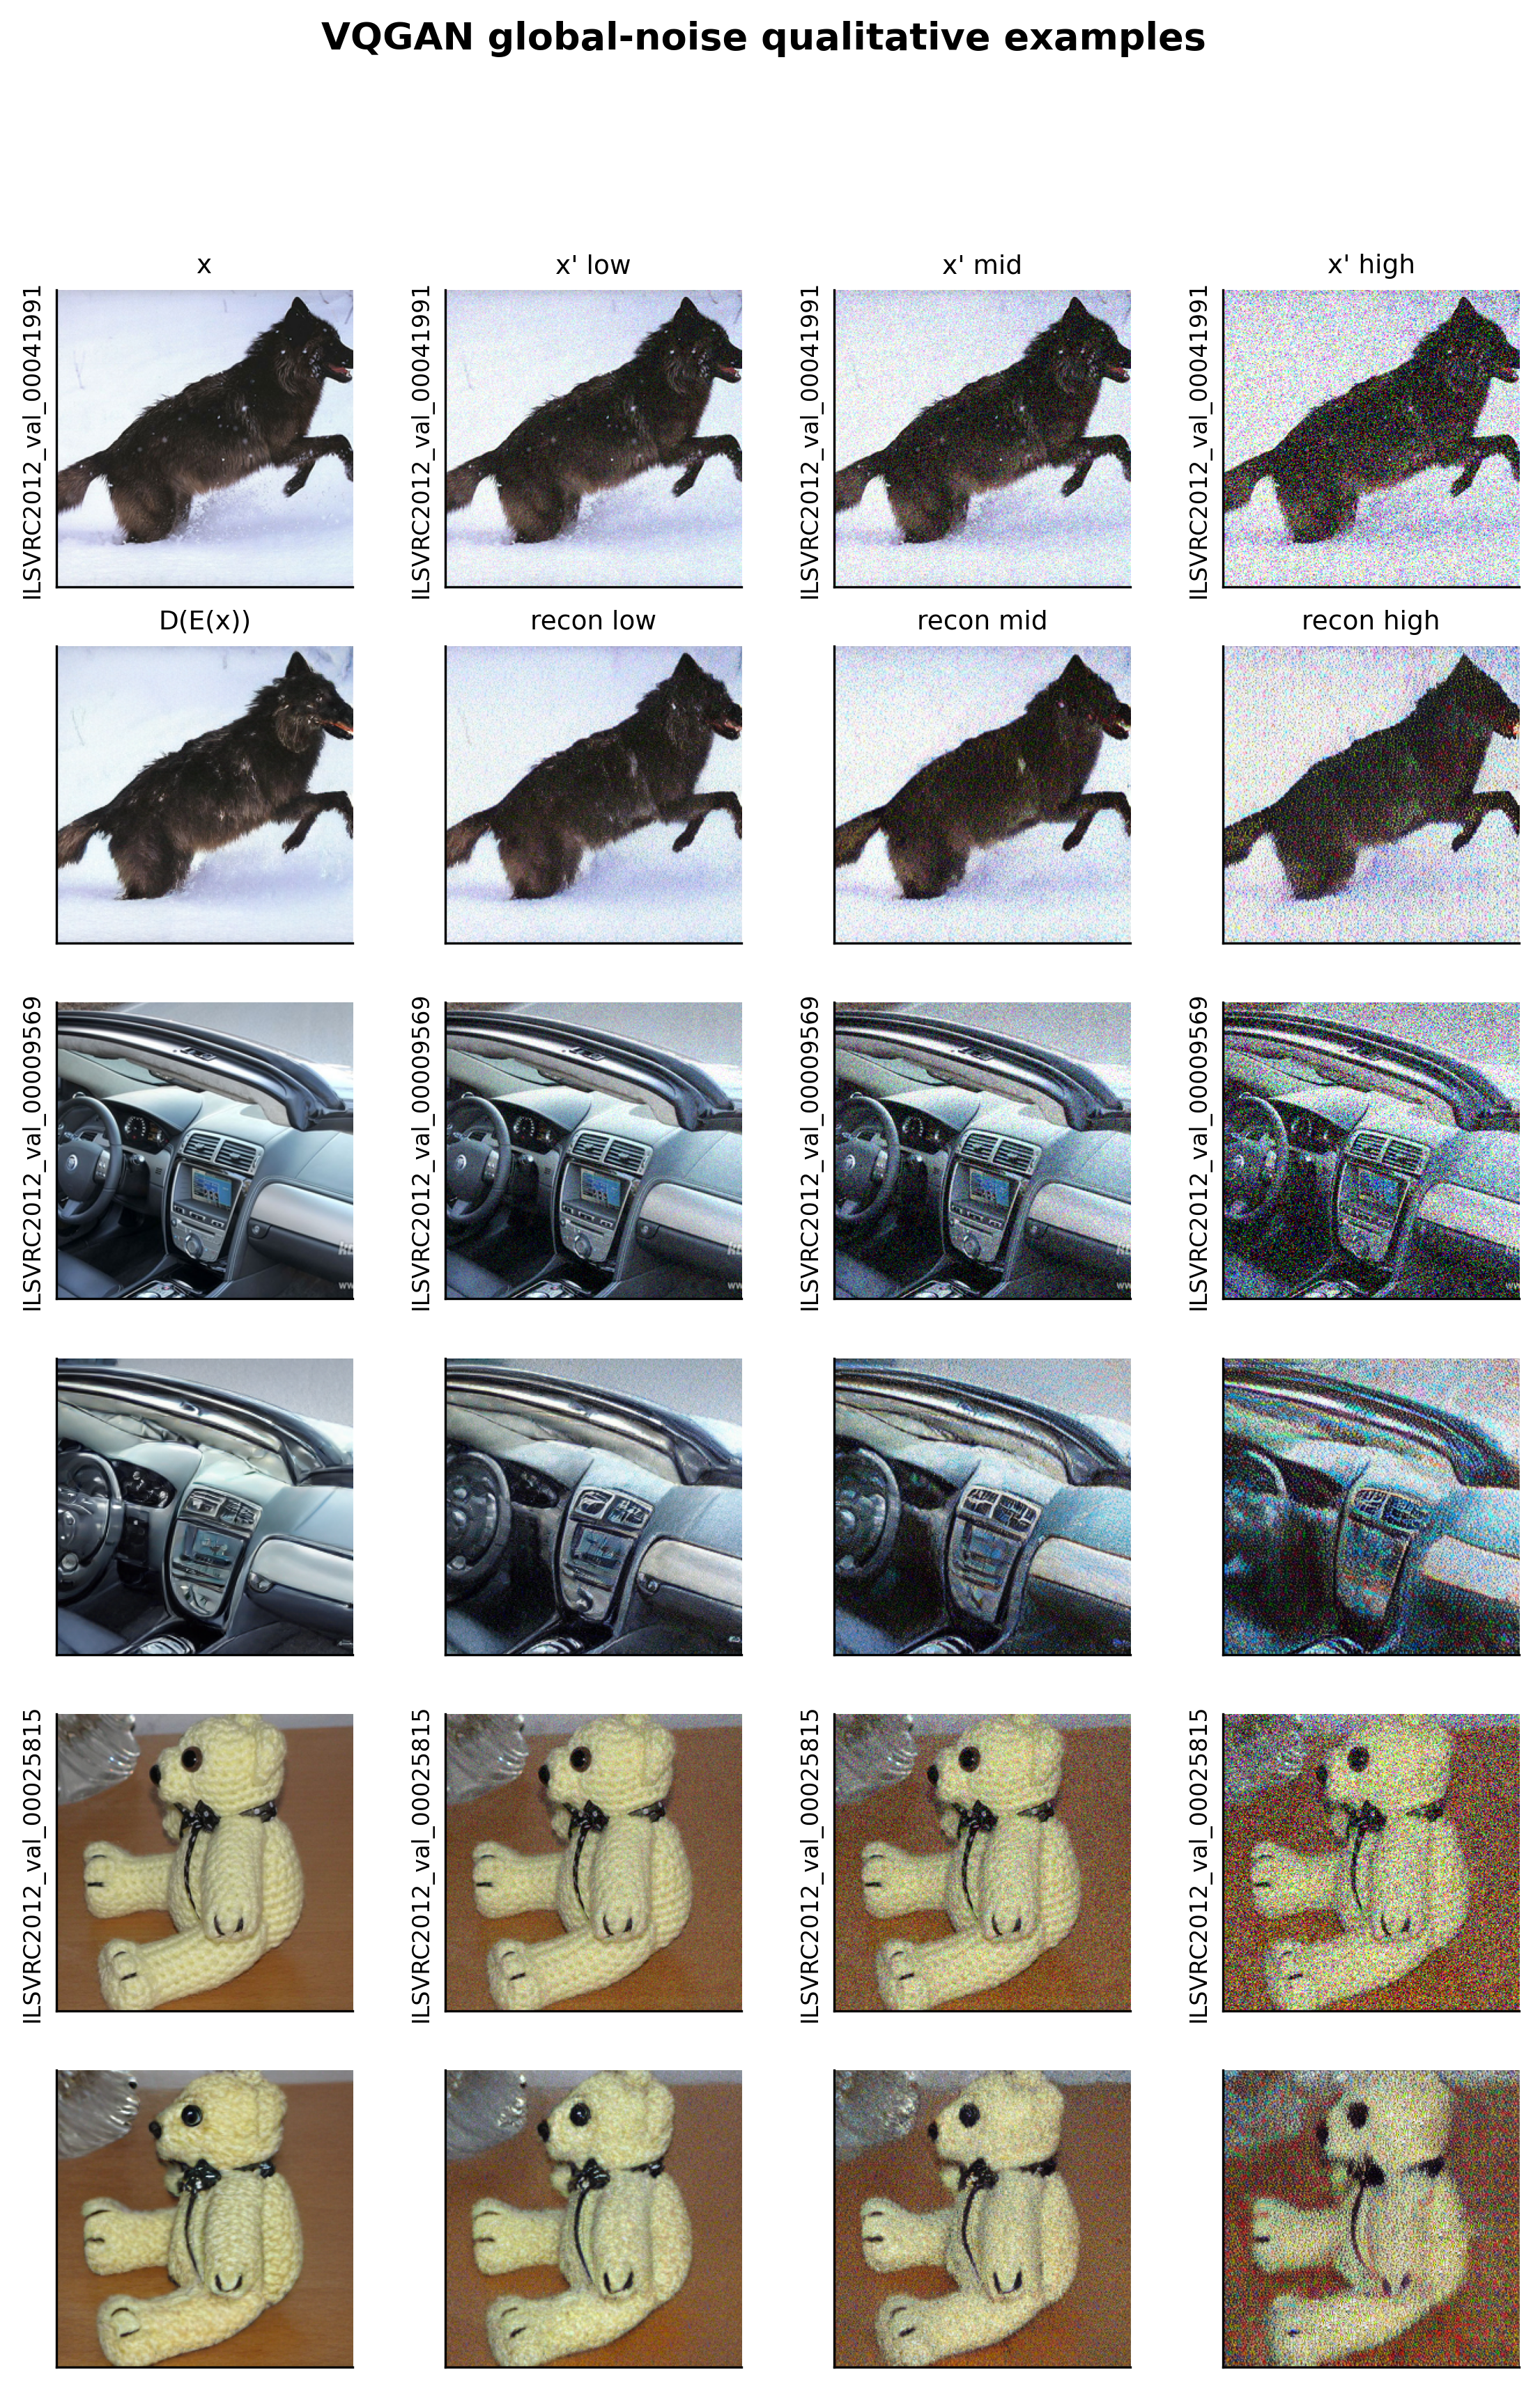
\includegraphics[width=0.94\textwidth,height=0.36\textheight,keepaspectratio]{ch05_fig_global_noise_qualitative_vqgan.png}\\[6pt]
    \textbf{(b) LlamaGen}\\[2pt]
    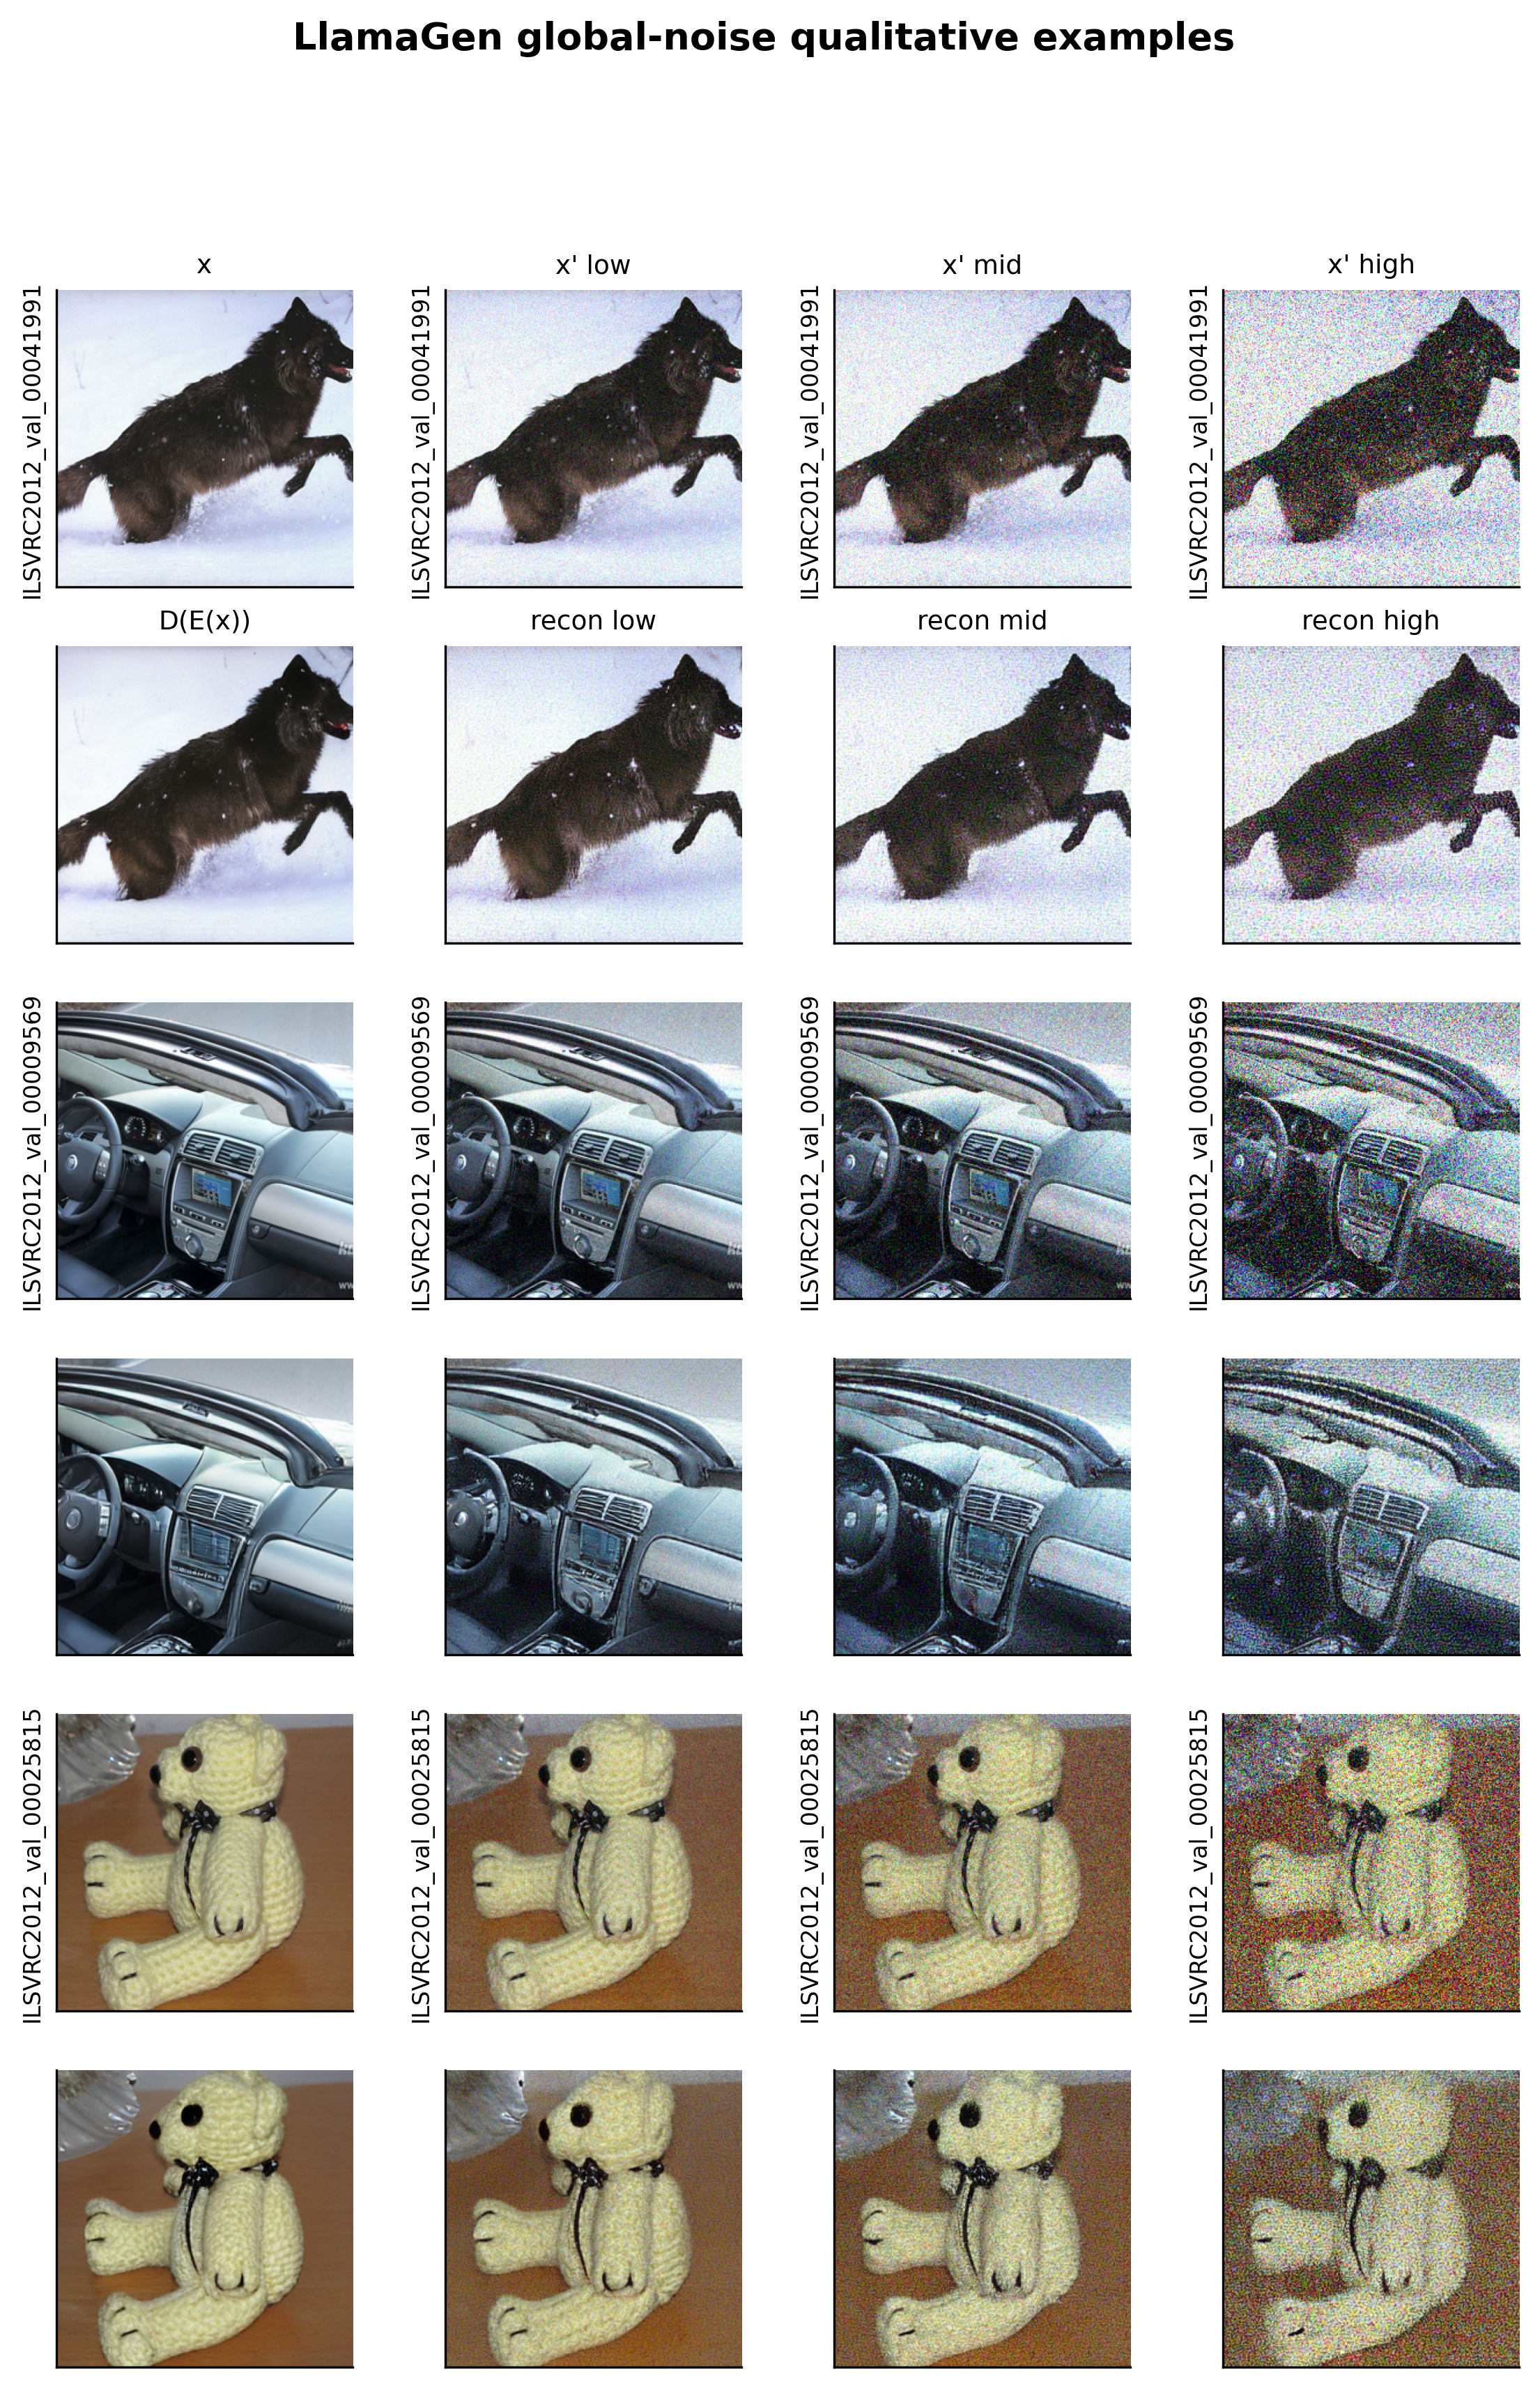
\includegraphics[width=0.94\textwidth,height=0.36\textheight,keepaspectratio]{ch05_fig_global_noise_qualitative_llamagen.png}
    \caption{Selected reconstructions under global Gaussian noise. Both panels
    use the same ImageNet samples and show $\sigma=0.1$, $0.2$, and $0.5$.}
    \label{fig:rq2_qual_combined}
\end{figure}
\subsection{Reconstruction Degradation}
\label{subsec:rq2_image_space}

Table~\ref{tab:rq2_psnr_summary} reports $\mathrm{PSNR}(x,\hat{x}_{\sigma})$, the end-to-end fidelity of the noisy-input reconstruction to the original clean image. Figure~\ref{fig:rq2_psnr_x_xhat} visualizes the same trend. Both tokenizers degrade monotonically as $\sigma$ increases, and LlamaGen remains above VQGAN at every level. At the clean baseline, LlamaGen reaches $20.79$ dB and VQGAN reaches $19.65$ dB. At the highest perturbation level, LlamaGen remains at $16.22$ dB, while VQGAN falls to $14.90$ dB.

The clean reconstruction difference persists under the tested perturbations.
The gaps are 1.14, 1.09, 1.00, and 1.32 dB from $\sigma=0$ to $0.5$, so they are
broadly similar rather than monotonically widening.

\begin{table}[t]
    \centering
    \small
    \begin{tabular}{llrr}
        \textbf{Tokenizer} & \textbf{Noise level} & $\boldsymbol{\sigma}$ & $\boldsymbol{\mathrm{PSNR}(x,\hat{x}_{\sigma})}$ \\ \hline
        LlamaGen & clean & 0.0 & $20.79 \pm 3.18$ \\
        LlamaGen & low & 0.1 & $20.32 \pm 2.71$ \\
        LlamaGen & mid & 0.2 & $19.11 \pm 1.98$ \\
        LlamaGen & high & 0.5 & $16.22 \pm 0.94$ \\
        \hline
        VQGAN & clean & 0.0 & $19.65 \pm 3.41$ \\
        VQGAN & low & 0.1 & $19.23 \pm 2.92$ \\
        VQGAN & mid & 0.2 & $18.11 \pm 2.27$ \\
        VQGAN & high & 0.5 & $14.90 \pm 1.03$ \\
    \end{tabular}
    \caption{End-to-end reconstruction fidelity under global Gaussian perturbations. Values are mean PSNR in dB $\pm$ standard deviation over 50{,}000 ImageNet validation images.}
    \label{tab:rq2_psnr_summary}
\end{table}
\begin{figure}[t]
    \centering
    
\includegraphics[width=0.86\textwidth]{ch05_fig_psnr_x_xhat_vs_sigma.png}
    \caption{Reconstruction fidelity to the clean input. Points show mean
    $\mathrm{PSNR}(x,\hat{x}_{\sigma})$ and error bars show one standard
    deviation across images. The horizontal axis is $\sigma$ and PSNR is in dB.}
    \label{fig:rq2_psnr_x_xhat}
\end{figure}
Figure~\ref{fig:rq2_psnr_xnoisy_xhat} reports
$\mathrm{PSNR}(x_{\sigma},\hat{x}_{\sigma})$. At $\sigma=0.1$, the values are
$19.26$ dB for LlamaGen and $18.36$ dB for VQGAN, a $0.90$ dB gap. At
$\sigma=0.5$, they are $11.87$ and $11.31$ dB, a $0.56$ dB gap. LlamaGen has a
modest advantage under this measure.

\begin{figure}[t]
    \centering
    
\includegraphics[width=0.86\textwidth]{ch05_fig_psnr_xnoisy_xhat_vs_sigma.png}
    \caption{PSNR between noisy input $x_{\sigma}$ and reconstruction $\hat{x}_{\sigma}$. This separates fidelity to the corrupted input from fidelity to the original clean image.}
    \label{fig:rq2_psnr_xnoisy_xhat}
\end{figure}
\subsection{Token Instability}
\label{subsec:rq2_token_flip}

The degradation in image space is gradual, while quantization can cause abrupt
assignment changes. Table~\ref{tab:rq2_token_flip} and
Figure~\ref{fig:rq2_token_flip} report the dataset mean of
$\mathrm{flip}_{\sigma}(x)$. At $\sigma=0.1$, VQGAN changes $75.1\%$ of token
positions and LlamaGen changes $79.5\%$, even though the selected
reconstructions remain recognizable. The latter is a qualitative observation.
At $\sigma=0.2$, the mean flip rates rise to $89.0\%$ and $91.0\%$; at
$\sigma=0.5$, both exceed $97\%$.

LlamaGen reconstructs better in image space, yet its mean flip rate is slightly
higher than VQGAN's at every tested level. This implies that reconstruction
quality and assignment stability describe different responses to noise.

\begin{table}[t]
    \centering
    \small
    \begin{tabular}{llrr}
        \textbf{Tokenizer} & \textbf{Noise level} & $\boldsymbol{\sigma}$ & \textbf{Token flip rate} \\ \hline
        LlamaGen & low & 0.1 & $0.795 \pm 0.099$ \\
        LlamaGen & mid & 0.2 & $0.910 \pm 0.054$ \\
        LlamaGen & high & 0.5 & $0.979 \pm 0.017$ \\
        VQGAN & low & 0.1 & $0.751 \pm 0.103$ \\
        VQGAN & mid & 0.2 & $0.890 \pm 0.057$ \\
        VQGAN & high & 0.5 & $0.975 \pm 0.017$ \\
    \end{tabular}
    \caption{Fraction of token positions changed relative to the clean tokenization. Values are mean $\pm$ standard deviation over ImageNet validation images.}
    \label{tab:rq2_token_flip}
\end{table}
\begin{figure}[t]
    \centering
    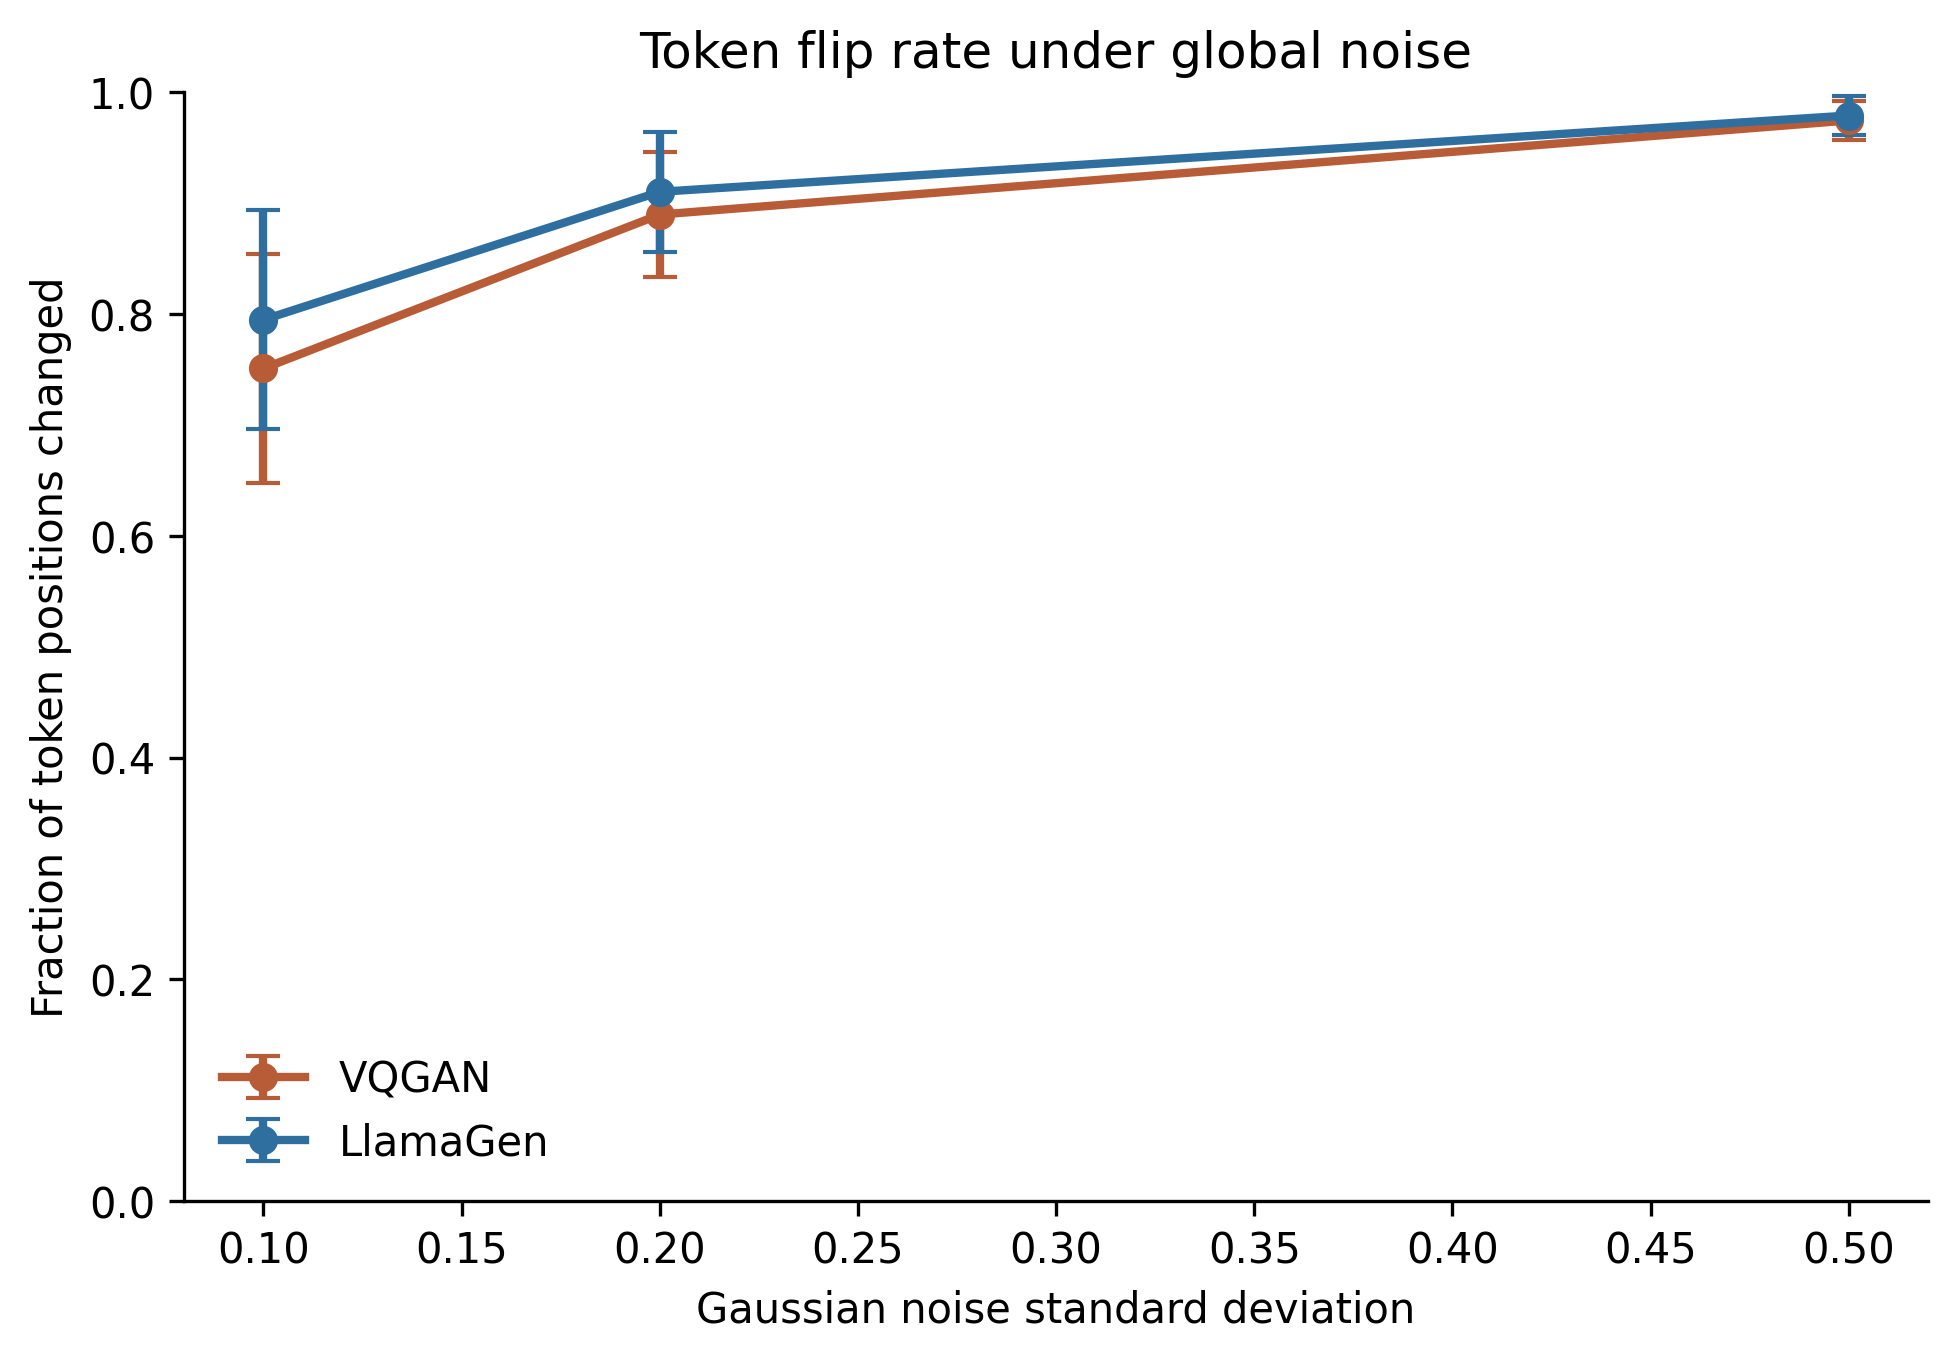
\includegraphics[width=0.86\textwidth]{ch05_fig_token_flip_vs_sigma.png}
    \caption{Token flip rate under global Gaussian perturbations. The discrete token representation changes sharply even when the image-space reconstruction remains visually structured.}
    \label{fig:rq2_token_flip}
\end{figure}
\subsection{Global Codebook Distribution}
\label{subsec:rq2_codebook_distribution}

After measuring changes at individual positions, we aggregate assignments
across images to examine code-frequency changes.
Table~\ref{tab:rq2_codebook_distribution} summarizes active-code counts,
perplexity, and top-$k$ concentration; Figure~\ref{fig:rq2_perplexity}
visualizes the main trend. Figure~\ref{fig:rq2_code_frequency_comparison}
compares clean and $\sigma=0.5$ assignment frequencies for the same codes.

The two tokenizers have different baselines. LlamaGen uses the full codebook on
clean ImageNet, with 16{,}384 active codes and a perplexity of 16{,}179. VQGAN
uses 972 active codes, with a perplexity of 910. Under noise, LlamaGen's active
count remains high and reaches 16{,}203 at $\sigma=0.5$; VQGAN's stays near 972.

Perplexity is more sensitive than active-code count. LlamaGen's perplexity decreases from 16{,}179 to 6{,}434 as $\sigma$ increases from 0 to 0.5. VQGAN's perplexity decreases from 910 to 560. Thus, both distributions become more concentrated even when the number of active codes changes little. The top-100 mass confirms this concentration: LlamaGen increases from 0.012 to 0.115, while VQGAN increases from 0.165 to 0.388.

\begin{table}[t]
    \centering
    \small
    \begin{tabular}{llrrrr}
        \textbf{Tokenizer} & \textbf{Level} & \textbf{Active codes} & \textbf{Perplexity} & \textbf{Top-100 mass} & \textbf{Top-1000 mass} \\ \hline
        LlamaGen & clean & 16{,}384 & 16{,}179 & 0.012 & 0.084 \\
        LlamaGen & low & 16{,}381 & 12{,}829 & 0.040 & 0.198 \\
        LlamaGen & mid & 16{,}369 & 10{,}388 & 0.063 & 0.269 \\
        LlamaGen & high & 16{,}203 & 6{,}434 & 0.115 & 0.416 \\
        \hline
        VQGAN & clean & 972 & 910 & 0.165 & 1.000 \\
        VQGAN & low & 973 & 859 & 0.202 & 1.000 \\
        VQGAN & mid & 971 & 780 & 0.249 & 1.000 \\
        VQGAN & high & 972 & 560 & 0.388 & 1.000 \\
    \end{tabular}
    \caption{Global codebook distribution statistics under global perturbations. Top-$k$ mass is the fraction of all token assignments explained by the $k$ most frequent codes at that noise level.}
    \label{tab:rq2_codebook_distribution}
\end{table}
\begin{figure}[t]
    \centering
    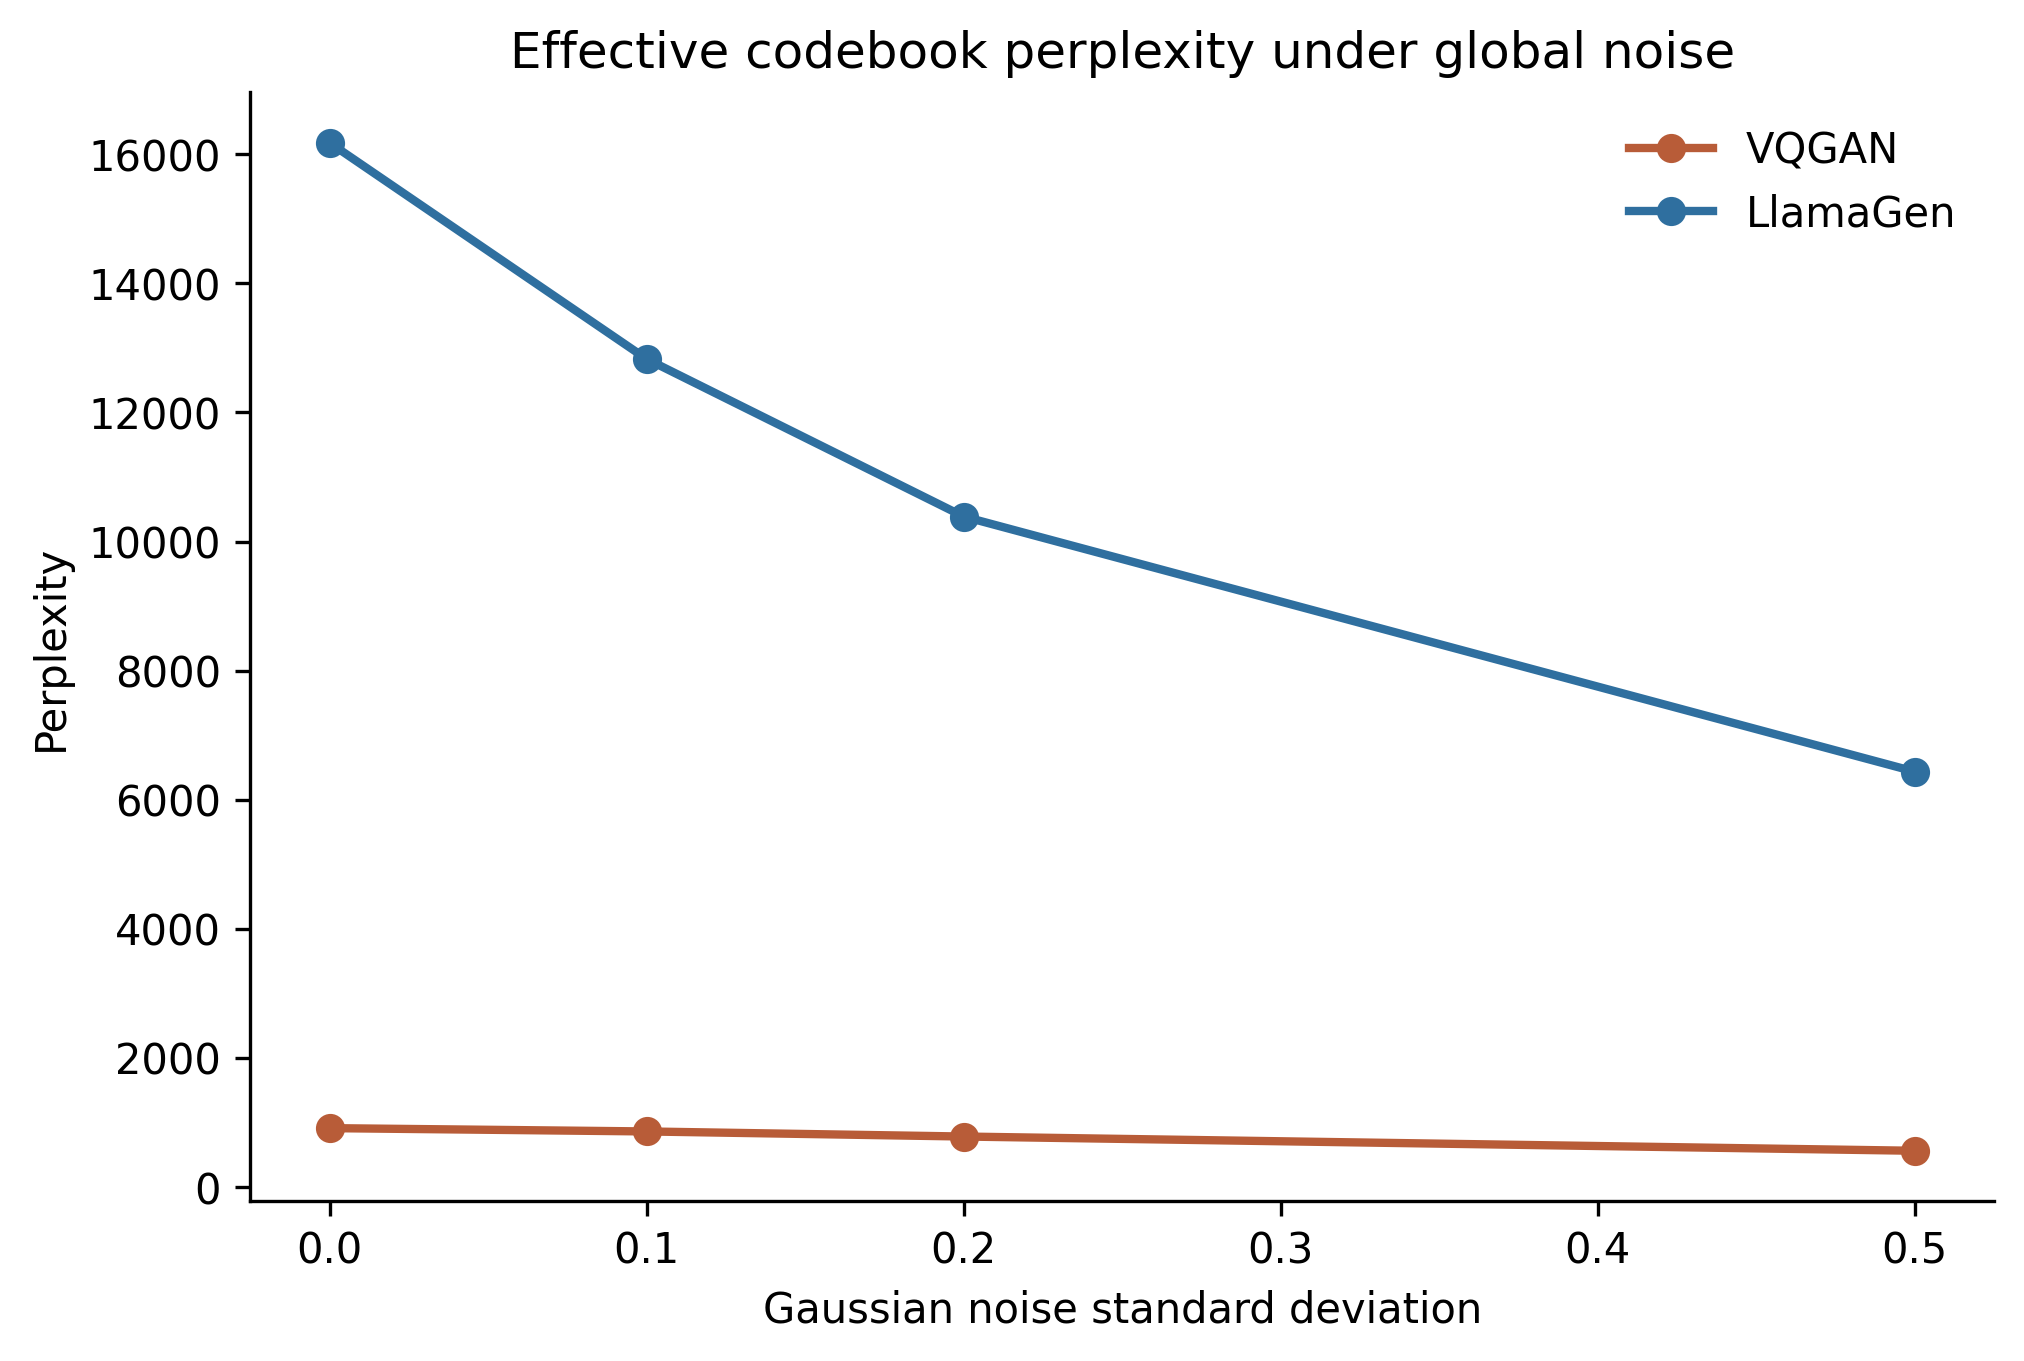
\includegraphics[width=0.86\textwidth]{ch05_fig_perplexity_vs_sigma.png}
    \caption{Effective codebook perplexity under global perturbations. LlamaGen remains much broader than VQGAN, but its effective vocabulary contracts substantially as noise increases.}
    \label{fig:rq2_perplexity}
\end{figure}
\begin{figure}[t]
    \centering
    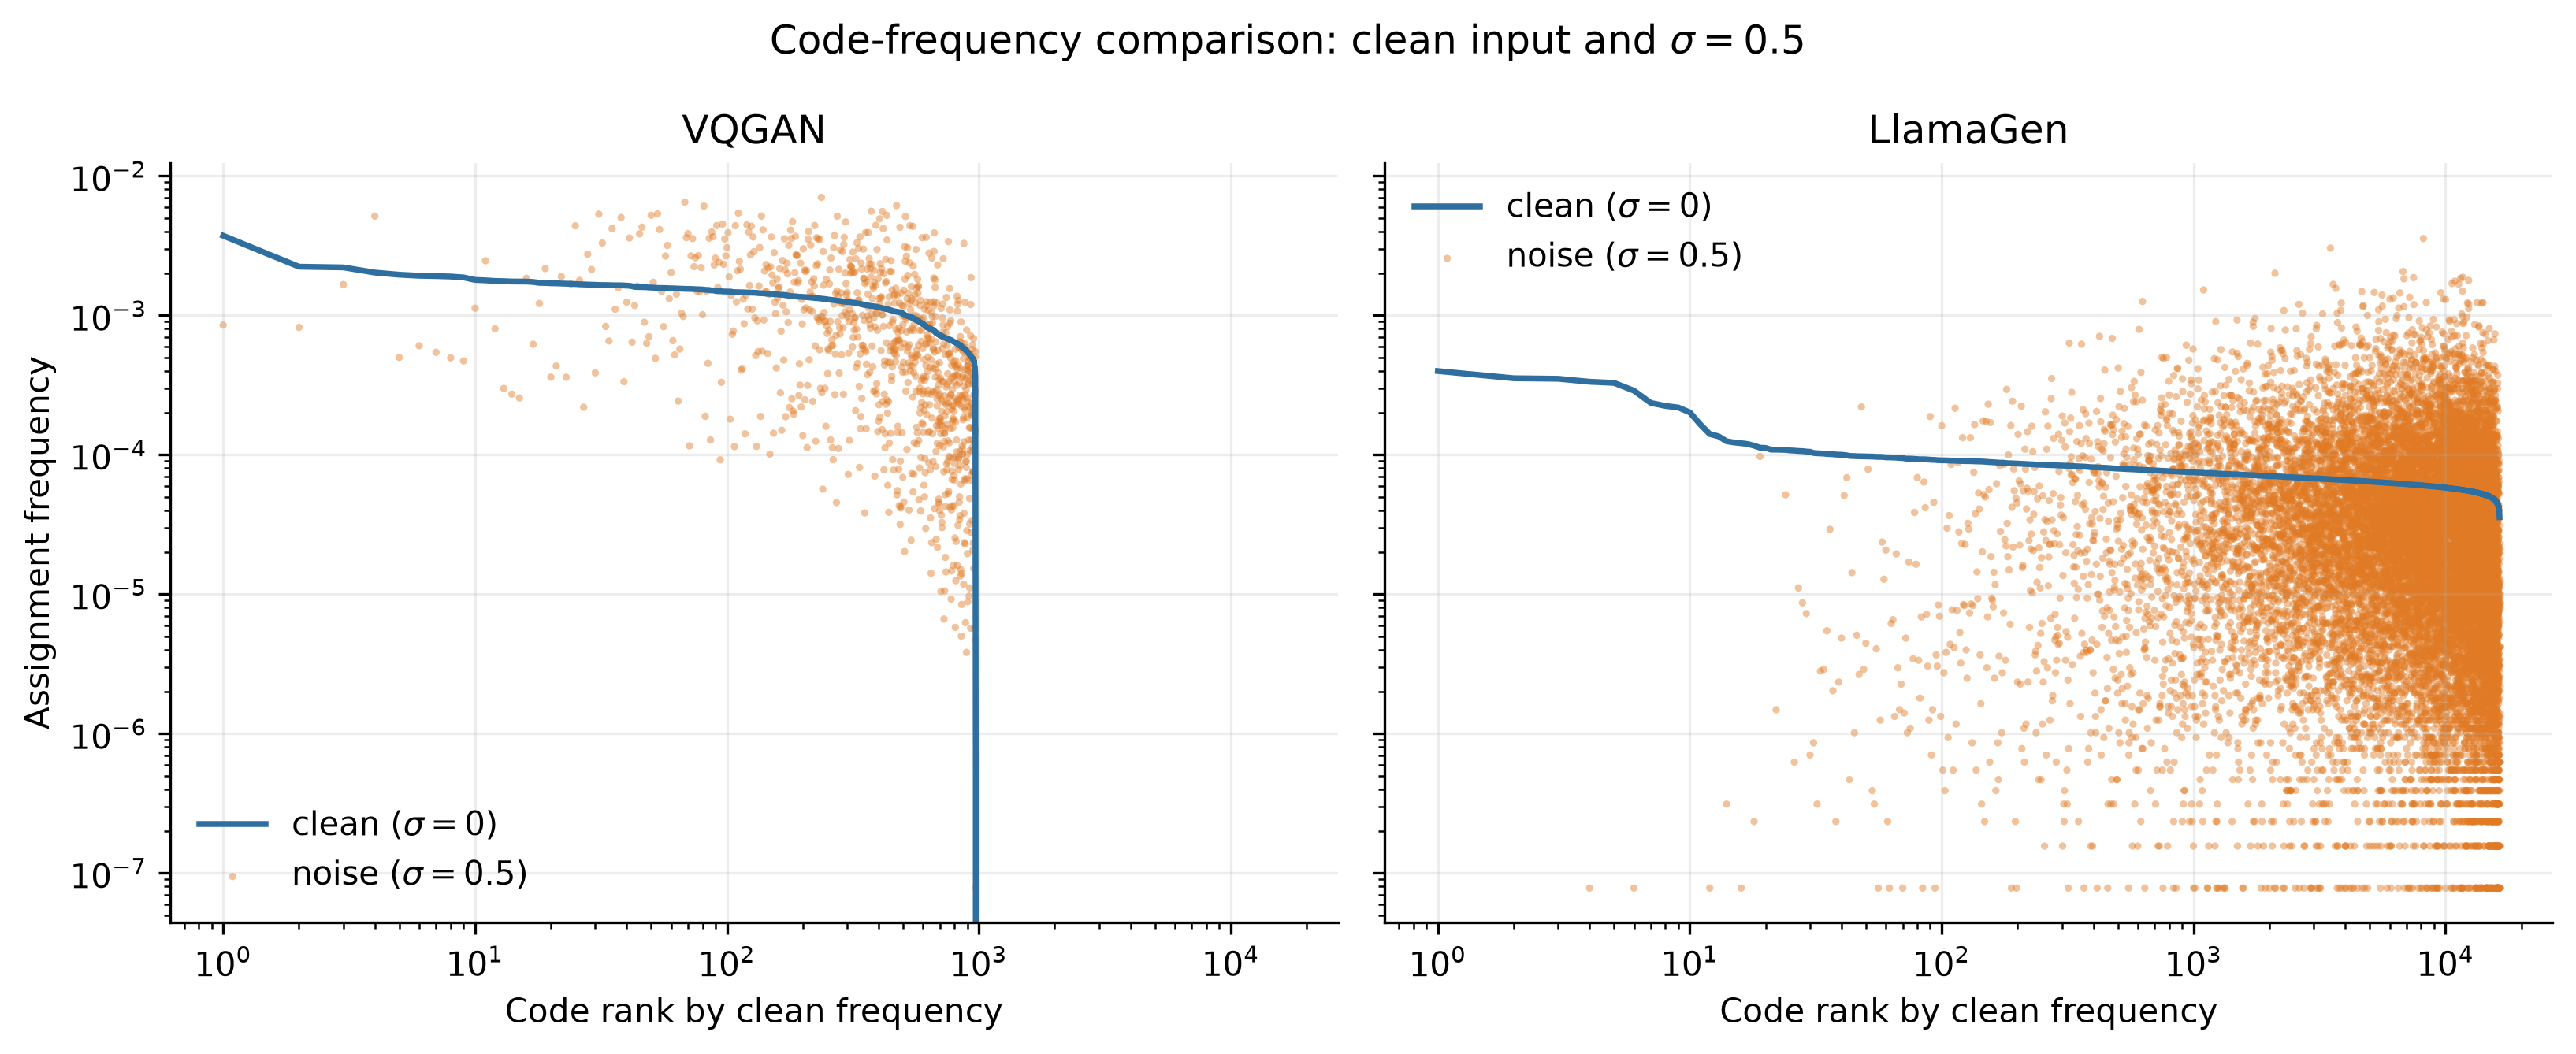
\includegraphics[width=0.96\textwidth]{ch05_fig_code_frequency_clean_vs_sigma_0_5.png}
    \caption{Per-code assignment frequencies for clean inputs and $\sigma=0.5$. Within each tokenizer, codes are ordered once by their clean frequency; the noisy points retain that fixed code ordering.}
    \label{fig:rq2_code_frequency_comparison}
\end{figure}
\section{Discussion}
\label{sec:rq2_discussion}

\paragraph{Reconstruction and assignment response.}
\label{subsec:rq2_reconstruction_token_divergence}

The two tokenizers show different responses in reconstruction quality and token
assignments. LlamaGen has higher PSNR at every tested level, yet its token flip
rate is slightly above VQGAN's.

One possible explanation is codebook geometry, but this experiment does not
measure feature displacements or distances to codebook boundaries. Measuring
those quantities is future work.

These assignment changes alter the sequences supplied to an autoregressive
model. Their effect on generator robustness remains a hypothesis. The
observations suggest that exact assignments can be sensitive even when selected
reconstructions remain recognizable; they do not establish whether individual
tokens carry stable semantics.

\paragraph{Code-frequency concentration.}
\label{subsec:rq2_noise_concentrates_usage}

Perplexity decreases and top-100 mass increases for both tokenizers while
active-code counts change comparatively little. The frequency distributions
therefore become more concentrated under noise.

The results above provide the reference point for the locality analyses. Global
noise perturbs all image regions. Chapter~\ref{ch:rq3} isolates a local image
change, and Chapter~\ref{ch:rq4} studies bounded token edits. These experiments
separate where a response occurs, but do not identify individual causal
mechanisms.

\chapter{Local Perturbations in Image Space}
\label{ch:rq3}

Global perturbations mix the response associated with one token's corresponding
image region with responses caused by changes elsewhere. This chapter perturbs
one image patch and measures how far assignment changes spread beyond it.
Chapter~\ref{ch:rq2} showed assignment instability under global noise; the
present experiment tests whether changes also appear outside a bounded patch.

Finite convolutional receptive fields create overlapping local dependencies,
while attention and spatial normalization can couple distant positions. The
evaluated VQGAN contains $3\times3$ stride-2 downsampling, $3\times3$ residual
convolutions, GroupNorm, and attention at its lowest-resolution level. These
facts identify candidate mechanisms, not the cause of the measured response.

\section{Experimental Setup}
\label{sec:rq3_setup}

\subsection{Patch-Noise Protocol}
\label{subsec:rq3_patch_noise_protocol}

Let $x \in [-1,1]^{H \times W \times 3}$ be an input image and let $P$ denote
a square patch. The binary mask $M_P$ equals one inside the patch and zero
outside it. For a noise level $\sigma$, the perturbed image is
\begin{equation}
    x_{\sigma,P}
    =
    \mathrm{clip}\!\left(x + \sigma \epsilon \odot M_P, -1, 1\right),
    \qquad
    \epsilon \sim \mathcal{N}(0,I).
    \label{eq:rq3_patch_noise}
\end{equation}
Only pixels inside $P$ receive additive noise. The clipping operation keeps the image in the valid pixel range.

Both tokenizers produce a $16\times16$ token grid. The analysis uses an
$8\times8$ token-space patch, corresponding to a $128\times128$ pixel region.
Its top-left corner is sampled uniformly from valid grid locations for each of
the 50,000 ImageNet validation images. The reported levels are
$\sigma\in\{0.1,0.25,0.5\}$. The two runs use the same images and nominal
settings but different random patch locations and noise realizations. Strictly
paired model comparisons would require shared perturbations and a rerun.

The masked variant fills the selected patch with black in the internal image
range. With fill value $c=-1$, it is defined as
\begin{equation}
    x_{\mathrm{mask},P}=(1-M_P)\odot x + M_P\odot c.
    \label{eq:rq3_patch_mask}
\end{equation}

\subsection{Inside and Outside Response}
\label{subsec:rq3_inside_outside_metrics}

Let $z_0 \in \{1,\ldots,K\}^{16 \times 16}$ be the clean token grid and $z_{\sigma,P}$ be the token grid obtained from the patch-perturbed image. Let $I_P$ be the set of token positions covered by the patch and let $O_P$ be the complement. We define the inside response as the fraction of token assignments within the selected patch that change:
\begin{equation}
    R_{\mathrm{in}}(\sigma,P)
    =
    \frac{1}{|I_P|}
    \sum_{i \in I_P}
    \mathbf{1}\!\left[z_{\sigma,P,i} \neq z_{0,i}\right].
    \label{eq:rq3_inside_response}
\end{equation}
We define the outside response as the fraction of token assignments outside the selected patch that change:
\begin{equation}
    R_{\mathrm{out}}(\sigma,P)
    =
    \frac{1}{|O_P|}
    \sum_{i \in O_P}
    \mathbf{1}\!\left[z_{\sigma,P,i} \neq z_{0,i}\right].
    \label{eq:rq3_outside_response}
\end{equation}
We define the encoder leakage ratio as
\begin{equation}
    \lambda_{\mathrm{enc}}(\sigma,P)
    =
    \frac{R_{\mathrm{out}}(\sigma,P)}
         {R_{\mathrm{in}}(\sigma,P) + \varepsilon}
    \label{eq:rq3_leakage_ratio}
\end{equation}
where $\varepsilon>0$ prevents division by zero. All responses are fractions of
token assignments that differ from the clean encoding. A value of
$\lambda_{\mathrm{enc}}$ near zero indicates that changes are mostly confined
to the patch, while a value near one indicates similar change rates inside and
outside it. We retain $R_{\mathrm{in}}$ and $R_{\mathrm{out}}$ alongside the
ratio because the same ratio can arise from different absolute responses.

\subsection{Distance Profile}
\label{subsec:rq3_distance_metrics}

The inside and outside responses do not show how far token changes spread. Each
token position $i$ is therefore assigned a Manhattan grid distance $d(i,P)$ to
the nearest token in $I_P$: distance zero is inside the patch, distance one is
the first ring of neighboring token cells, and larger values move farther
across the token grid. We define the distance profile as
\begin{equation}
    R_d(\sigma,P)
    =
    \frac{1}{|\{i : d(i,P)=d\}|}
    \sum_{i : d(i,P)=d}
    \mathbf{1}\!\left[z_{\sigma,P,i} \neq z_{0,i}\right].
    \label{eq:rq3_distance_profile}
\end{equation}
The results report the full profile and a small set of bands: inside tokens ($d=0$), boundary-neighbor tokens ($d=1$), near tokens ($d \in \{1,2\}$), and far-field tokens ($d \geq 6$).

\section{Experimental Results}
\label{sec:rq3_results}

\paragraph{Qualitative patch perturbations.}
\label{subsec:rq3_qualitative}

Figure~\ref{fig:rq3_qual_combined} shows selected examples for the two tokenizers. Each panel contains the clean image, the patch-noisy inputs, the corresponding reconstructions, and binary token-response maps. The black rectangle marks the perturbed patch in pixel space and the corresponding token block in the response map. Highlighted cells outside the rectangle are token-assignment changes outside the patch.

\begin{figure}[tbp]
    \centering
    \textbf{(a) VQGAN}\par\smallskip
    
\includegraphics[width=\textwidth,height=0.35\textheight,keepaspectratio]{ch06_fig_patch_noise_qualitative_vqgan.png}
    \begin{minipage}{0.96\textwidth}
        \footnotesize\centering
        Sample ILSVRC2012\_val\_00000293:
        $\sigma=0.1$ ($R_{\mathrm{in}}=0.766$, $R_{\mathrm{out}}=0.297$, $\lambda_{\mathrm{enc}}=0.388$);
        $\sigma=0.25$ ($0.969$, $0.630$, $0.651$);
        $\sigma=0.5$ ($0.969$, $0.724$, $0.747$).
    \end{minipage}

    \medskip
    \textbf{(b) LlamaGen}\par\smallskip
    
\includegraphics[width=\textwidth,height=0.35\textheight,keepaspectratio]{ch06_fig_patch_noise_qualitative_llamagen.png}
    \begin{minipage}{0.96\textwidth}
        \footnotesize\centering
        Sample ILSVRC2012\_val\_00000293:
        $\sigma=0.1$ ($R_{\mathrm{in}}=0.875$, $R_{\mathrm{out}}=0.323$, $\lambda_{\mathrm{enc}}=0.369$);
        $\sigma=0.25$ ($0.938$, $0.526$, $0.561$);
        $\sigma=0.5$ ($0.984$, $0.656$, $0.667$).
    \end{minipage}
    \caption{Selected local patch-noise examples for (a) VQGAN and (b) LlamaGen using the same input ID. The binary response maps use dark cells for unchanged assignments (0) and yellow cells for changed assignments (1); the marked rectangle identifies the perturbed patch. Metrics below each panel are sample-specific and ordered as $R_{\mathrm{in}}$, $R_{\mathrm{out}}$, and $\lambda_{\mathrm{enc}}$.}
    \label{fig:rq3_qual_combined}
\end{figure}
\paragraph{Local response and leakage.}
\label{subsec:rq3_inside_outside_results}

Table~\ref{tab:rq3_inside_outside_summary} reports the mean inside response
$R_{\mathrm{in}}$, outside response $R_{\mathrm{out}}$, encoder leakage ratio
$\lambda_{\mathrm{enc}}$, and far-field response. A high inside response is
expected because the corresponding image pixels are directly perturbed. At
$\sigma=0.1$, VQGAN changes 78.8\% of inside assignments and LlamaGen changes
82.2\%. At $\sigma=0.5$, the inside response is almost saturated for both.

Token assignments also change outside the patch at the lowest tested level:
$R_{\mathrm{out}}$ is 29.9\% for VQGAN and 30.2\% for LlamaGen at
$\sigma=0.1$. It rises to 44.1\% and 42.8\%, respectively, at $\sigma=0.25$,
then to 52.1\% and 50.5\% at $\sigma=0.5$. At the largest tested value,
outside assignments change about half as often as inside assignments. A
lower-noise sweep would be needed to estimate when $R_{\mathrm{out}}$
approaches zero.

\begin{table}[t]
    \centering
    \small
    \begin{tabular}{lrrrrr}
        \textbf{Tokenizer} & $\boldsymbol{\sigma}$ & $\boldsymbol{R_{\mathrm{in}}}$ & $\boldsymbol{R_{\mathrm{out}}}$ & $\boldsymbol{\lambda_{\mathrm{enc}}}$ & \textbf{Far field} \\ \hline
        VQGAN & 0.10 & 0.788 & 0.299 & 0.375 & 0.174 \\
        VQGAN & 0.25 & 0.952 & 0.441 & 0.462 & 0.265 \\
        VQGAN & 0.50 & 0.988 & 0.521 & 0.527 & 0.333 \\ \hline
        LlamaGen & 0.10 & 0.822 & 0.302 & 0.361 & 0.178 \\
        LlamaGen & 0.25 & 0.960 & 0.428 & 0.444 & 0.260 \\
        LlamaGen & 0.50 & 0.991 & 0.505 & 0.509 & 0.328 \\
    \end{tabular}
    \caption{Inside and outside token response under local patch-noise perturbations. The far-field column reports the mean token flip rate for positions at distance at least six token cells from the perturbed patch.}
    \label{tab:rq3_inside_outside_summary}
\end{table}
\begin{figure}[t]
    \centering
    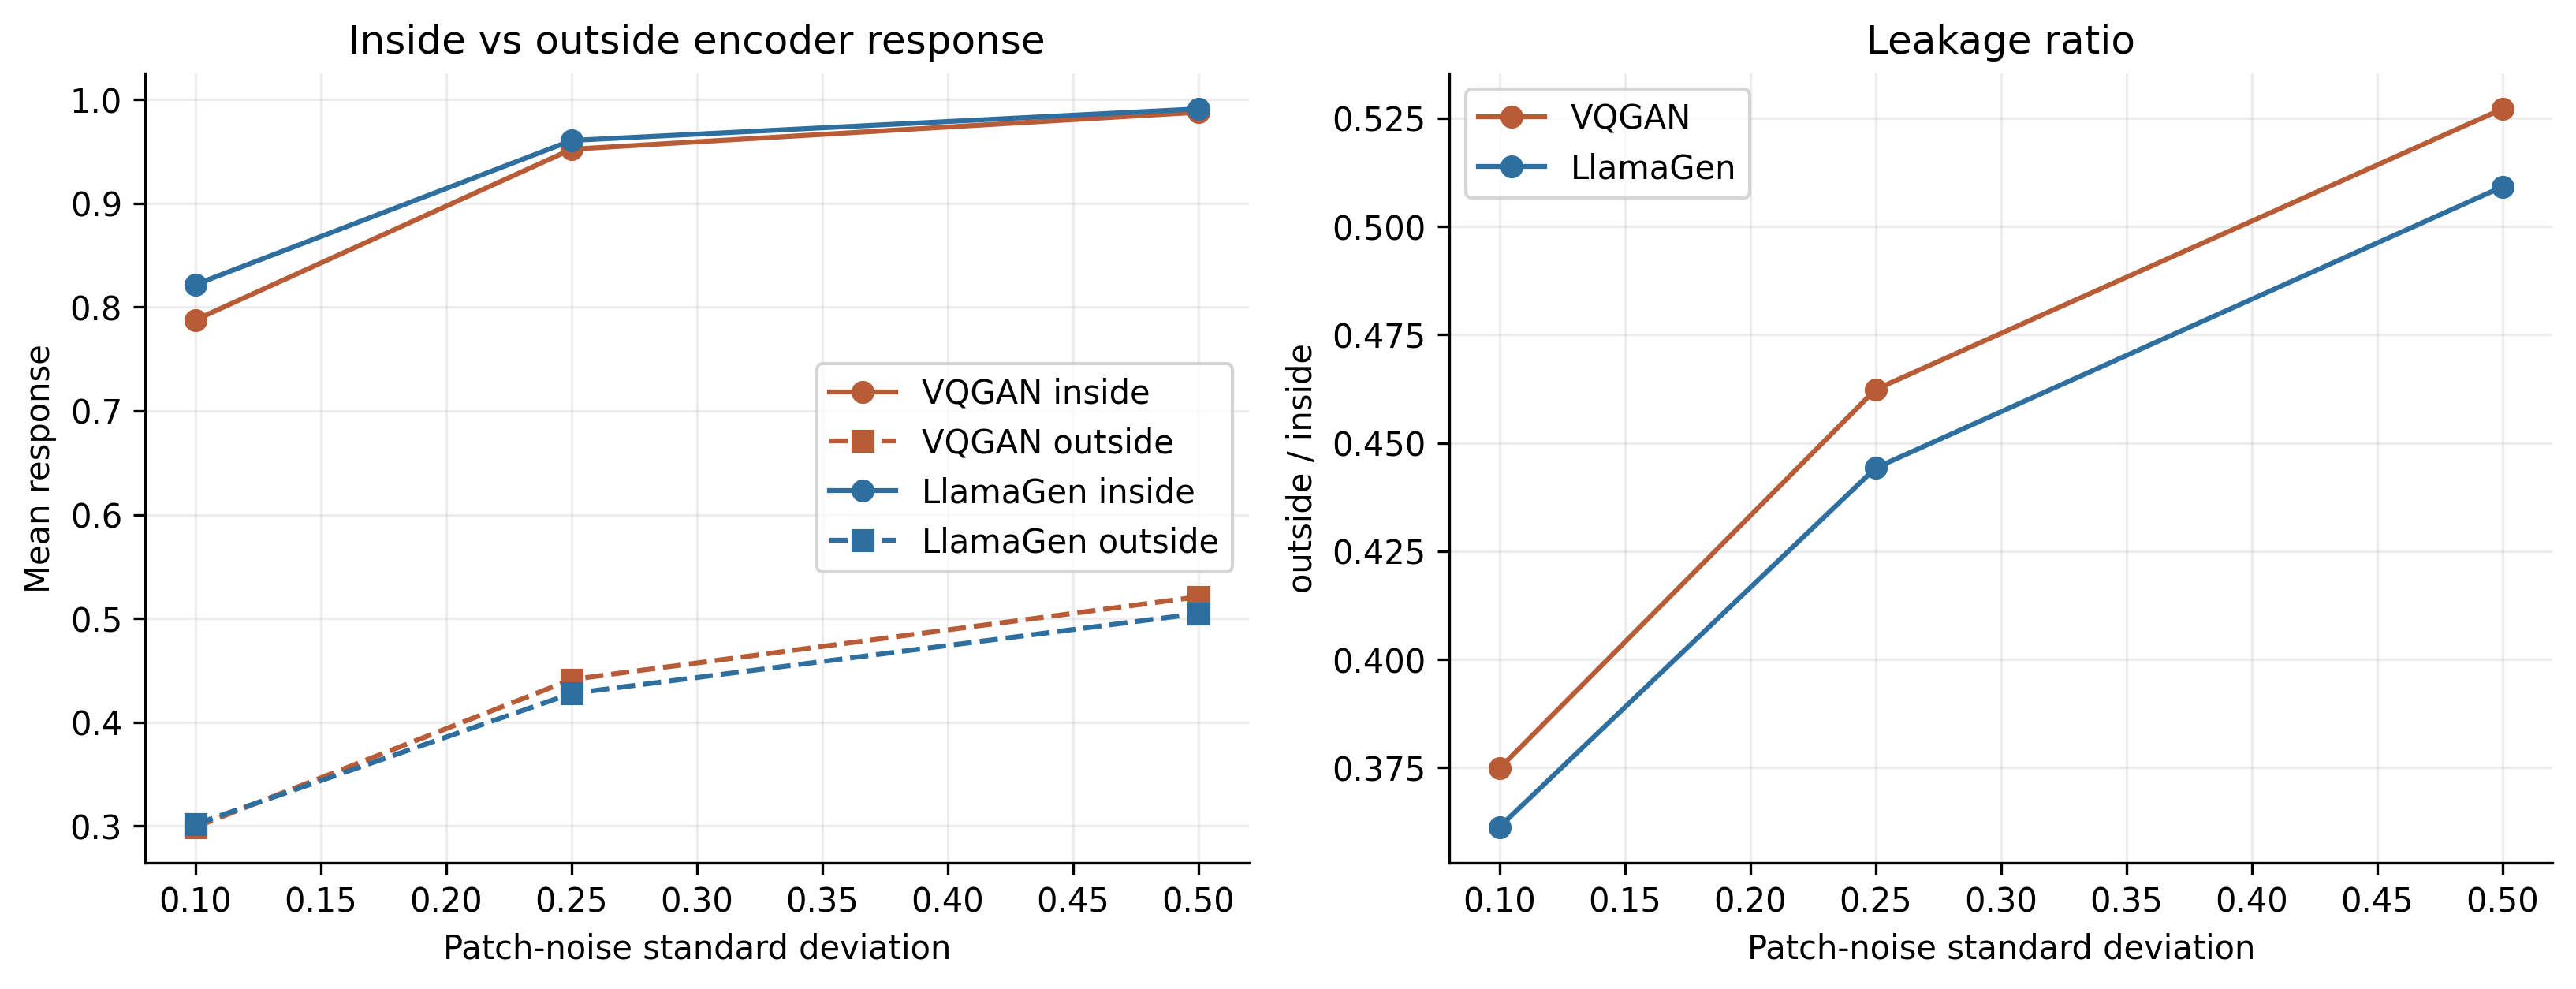
\includegraphics[width=0.92\textwidth]{ch06_fig_inside_outside_response.png}
    \caption{Mean token response inside and outside the perturbed patch, with the corresponding leakage ratio. Outside-token changes increase monotonically with noise level for both tokenizers, and the outside/inside ratio also increases.}
    \label{fig:rq3_inside_outside_response}
\end{figure}
\paragraph{Distance from the perturbed patch.}
\label{subsec:rq3_distance_results}

Figure~\ref{fig:rq3_distance_profile_flip} plots the response to the image
perturbation as a function of distance from the patch. It declines sharply over
the first few token cells but remains nonzero farther away. Table~\ref{tab:rq3_distance_band_summary}
summarizes the curves using descriptive distance bands. The chosen far-field
band, $d \geq 6$, separates distant positions from the immediate rings; it is
not a measured boundary between local and global mechanisms. In this band,
17.4\% of VQGAN assignments and 17.8\% of LlamaGen assignments change at
$\sigma=0.1$. At $\sigma=0.5$, the fraction is roughly one third.

\begin{table}[t]
    \centering
    \small
    \begin{tabular}{lrrrr}
        \textbf{Tokenizer} & $\boldsymbol{\sigma}$ & \textbf{Inside} & \textbf{Boundary} & \textbf{Far field} \\ \hline
        VQGAN & 0.10 & 0.788 & 0.597 & 0.174 \\
        VQGAN & 0.25 & 0.952 & 0.827 & 0.265 \\
        VQGAN & 0.50 & 0.988 & 0.917 & 0.333 \\ \hline
        LlamaGen & 0.10 & 0.822 & 0.613 & 0.178 \\
        LlamaGen & 0.25 & 0.960 & 0.832 & 0.260 \\
        LlamaGen & 0.50 & 0.991 & 0.922 & 0.328 \\
    \end{tabular}
    \caption{Distance-band summary of token response. Inside denotes $d=0$, boundary denotes $d=1$, and far field denotes positions with Manhattan distance $d \geq 6$ from the perturbed patch.}
    \label{tab:rq3_distance_band_summary}
\end{table}
\begin{figure}[t]
    \centering
    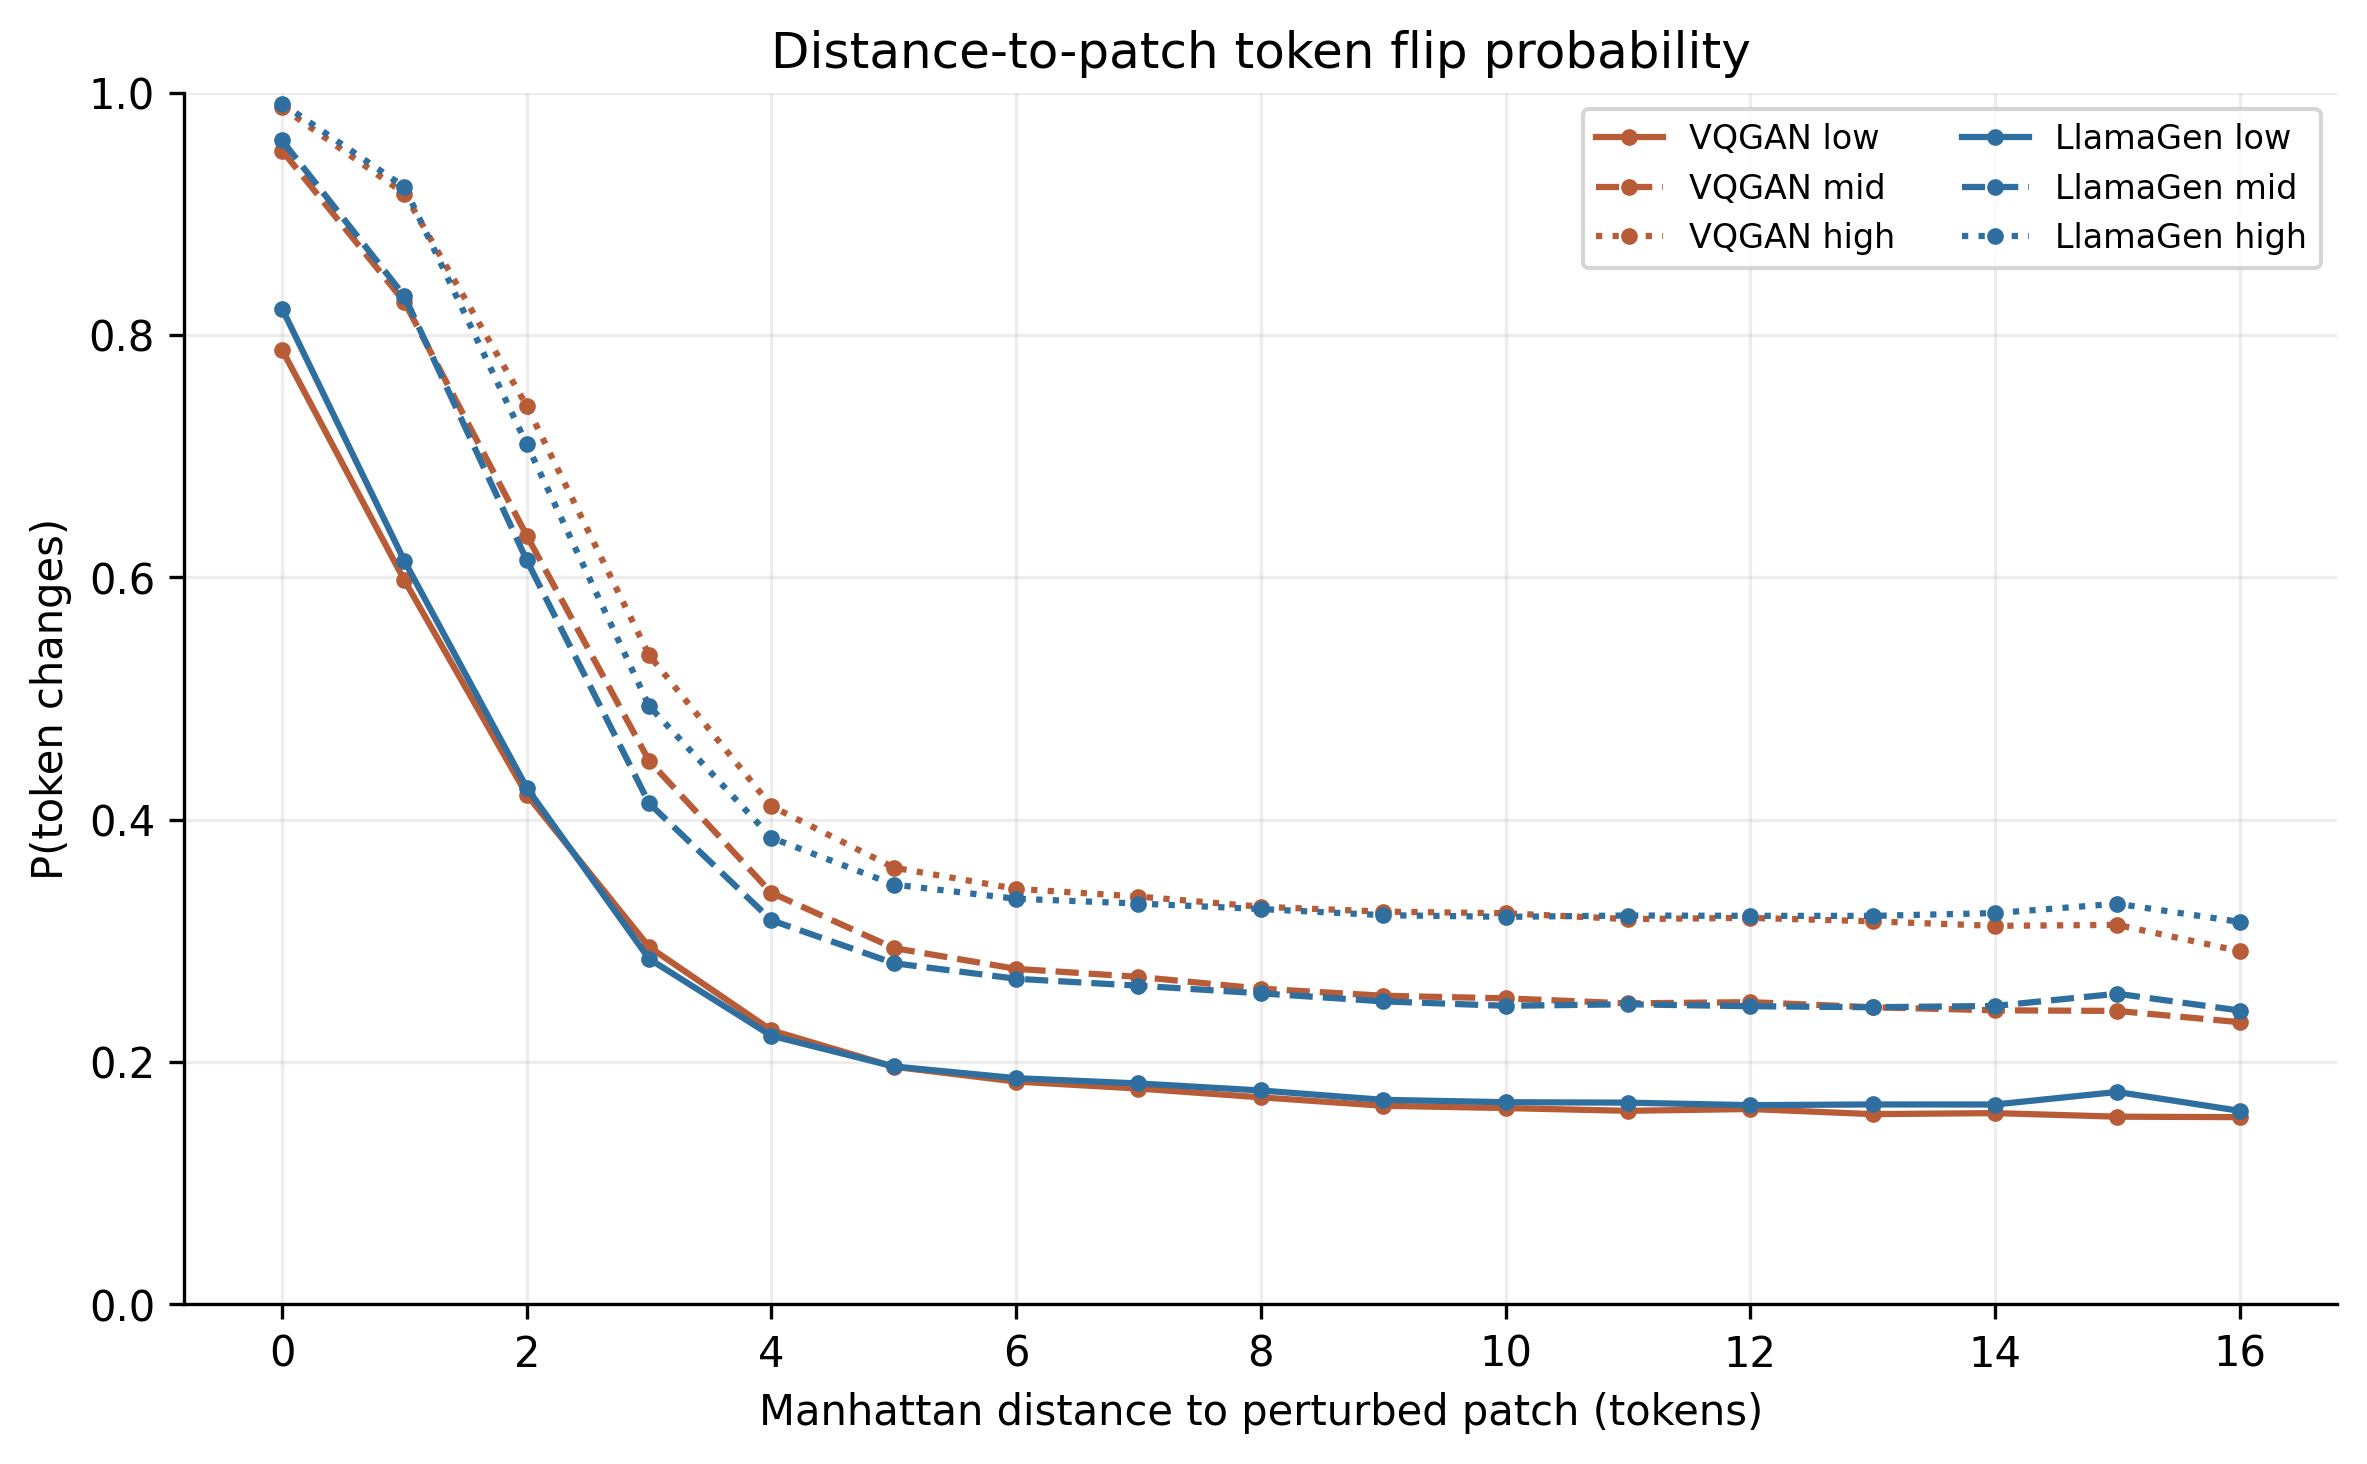
\includegraphics[width=0.86\textwidth]{ch06_fig_distance_profile_flip.png}
    \caption{Token flip probability as a function of distance from the perturbed patch. The response is strongest inside and near the patch, but remains measurable far from it.}
    \label{fig:rq3_distance_profile_flip}
\end{figure}
\paragraph{Masked patch intervention.}
\label{subsec:rq3_masked_results}

The masked intervention defined in Equation~\ref{eq:rq3_patch_mask} replaces the
same local patch with black. Table~\ref{tab:rq3_masked_summary} shows that this
nearly saturates the inside response for both tokenizers, while the response to
the image perturbation outside the patch is 56.3\% for VQGAN and 49.5\% for
LlamaGen. Thus, a change confined to one quarter of the image changes token
assignments across roughly half of the remaining grid.

\begin{table}[t]
    \centering
    \small
    \begin{tabular}{lrrr}
        \textbf{Tokenizer} & $\boldsymbol{R_{\mathrm{in}}}$ & $\boldsymbol{R_{\mathrm{out}}}$ & $\boldsymbol{\lambda_{\mathrm{enc}}}$ \\ \hline
        VQGAN & 0.998 & 0.563 & 0.564 \\
        LlamaGen & 1.000 & 0.495 & 0.495 \\
    \end{tabular}
    \caption{Inside and outside token response for the masked-patch intervention. The mask is a stronger local corruption than Gaussian patch noise and produces a correspondingly high outside response.}
    \label{tab:rq3_masked_summary}
\end{table}
\section{Discussion}
\label{sec:rq3_discussion}

Both tokenizers show the same measured pattern: token changes are most frequent
inside and near the perturbed patch, decline over the nearby token cells, and
remain nonzero at distant positions. LlamaGen has a slightly higher inside
response at $\sigma=0.1$ and a slightly lower leakage ratio at each tested
value, but the spatial pattern is shared.

The evaluated architecture contains overlapping $3\times3$ convolutions,
GroupNorm, and an attention layer. A small feature movement can also cross a
nearest-neighbor quantization boundary and change the assignment at that
position, although pointwise quantization does not transmit changes between
positions. The measurements do not isolate the contribution of these
components. Future work can investigate attention, spatial normalization, and
receptive-field overlap through ablations and intermediate-feature analysis.

This result complements Chapter~\ref{ch:rq2}. Global noise changed many token
assignments when every image region was perturbed. The study of perturbation
locality shows how far those changes spread when the image modification is
bounded: token assignments change well beyond the selected patch. These
changes also alter the token sequences supplied to an autoregressive model.

\chapter{Local Perturbations in Token Space}
\label{ch:rq4}

The previous chapter showed that a local image-space perturbation causes token changes well beyond the corrupted patch. This chapter examines the complementary decoder-side question: when token IDs inside a bounded region of the latent grid are replaced directly, how far does the decoded image change?

The experiment replaces token IDs inside a contiguous rectangular region and
measures the decoded change inside and outside the corresponding image region.
It asks how severe the change is and how far it extends beyond the edited patch.

A discrete image tokenizer represents an image as a spatial grid of codebook
indices. Editing a bounded region of this grid is expected to affect mainly
the corresponding region of the decoded image. Decoder locality matters because
autoregressive image models may make local token errors: if the decoder spreads
such errors widely, a local sequence error can become a broader image artifact.

The replacement strategies test whether nearby codebook vectors decode to
similar image content and whether more distant vectors cause larger changes.
Nearest-neighbour replacement tests a small change in the embedding space;
farthest replacement tests a large one. Orthogonal replacement selects a
vector with cosine similarity near zero, and random replacement provides a
reference independent of distance. We expect these strategies to produce
different levels of change, but their decoded effects must be measured.

\section{Experimental Setup}
\label{sec:rq4_setup}

\subsection{Token-Edit Protocol}
\label{subsec:rq4_token_edit_protocol}

Let $z_0 \in \{1,\ldots,K\}^{h \times w}$ denote the clean token grid produced
for an image, and let $B_{\mathrm{tok}}$ be a contiguous rectangular region of
that grid. For an edit mode $m$, the edited token grid $z^{(m)}$ is
\begin{equation}
    z^{(m)}_{i,j}
    =
    \begin{cases}
        T_m(z_{0,i,j}), & (i,j) \in B_{\mathrm{tok}}, \\
        z_{0,i,j}, & (i,j) \notin B_{\mathrm{tok}},
    \end{cases}
    \label{eq:rq4_token_edit}
\end{equation}
where $T_m$ maps the original token to a replacement token. The experiment
uses four mappings:
\begin{itemize}
    \item \textbf{Closest}: the nearest alternative codebook vector;
    \item \textbf{Orthogonal}: a codebook vector with cosine similarity close
          to zero;
    \item \textbf{Random}: a uniformly sampled codebook vector;
    \item \textbf{Farthest}: the most distant codebook vector.
\end{itemize}

For VQGAN, the
closest, orthogonal, and farthest mappings are restricted to the empirically
active code subset identified in Chapter~\ref{ch:rq1}. VQGAN uses only part of
its codebook on the reference dataset. Uniform-random
replacement is different: it samples from the full codebook for both models.
For VQGAN this means that random replacement may introduce inactive codes, so
the random edit tests both replacement and the use of previously inactive codes.

The clean and edited reconstructions are
\begin{equation}
    x_{\mathrm{clean}} = D(z_0),
    \qquad
    x_{\mathrm{edit}}^{(m)} = D(z^{(m)}),
    \label{eq:rq4_clean_edited_decode}
\end{equation}
where $D$ is the tokenizer decoder. All image changes are measured against
$x_{\mathrm{clean}}$, so ordinary reconstruction error relative to the input
does not enter the perturbation measurement.

The main comparisons use a patch covering $25\%$ of the token grid. A
patch-size sweep also tests target fractions of $10\%$, $50\%$, and $75\%$.
The main analysis uses
ImageNet validation; ImageNet-V2 is used to test whether the observed trends
remain stable under a natural distribution shift.

Images are resized and center-cropped to $256\times256$ using the
model-specific preprocessing described in Appendix~\ref{app:computational_environment}.
Decoder outputs are converted from the models' internal $[-1,1]$ range to
$[0,1]$ before metrics are computed. Patch locations
are reproducible within each run. The two tokenizers did not receive shared
random replacement draws, so comparisons describe aggregate behavior.

Both tokenizers produce a $16 \times 16$ grid. For each image, a square patch
is sampled at a random valid position for the largest target fraction. The
smaller patches are nested within that patch, so comparisons across fractions
do not also change the general image region being edited. The square side lengths are
5, 8, 11, and 14 tokens, corresponding to actual grid fractions of 9.8\%,
25.0\%, 47.3\%, and 76.6\%, respectively.

\subsection{Fidelity Metrics}
\label{subsec:rq4_fidelity_metrics}

Decoder locality alone does not describe the severity of an edit. A low
outside response may coincide with either a negligible local change or severe
damage confined to the patch. Using the definitions and metric references in
Chapter~\ref{ch:datasets_models_metrics}, the experiment measures PSNR, SSIM,
and LPIPS between $x_{\mathrm{clean}}$ and $x_{\mathrm{edit}}^{(m)}$, both over
the full image and within $B_{\mathrm{px}}$. Patch-level metrics quantify edit
severity; the inside/outside response and leakage ratio quantify spatial
propagation. The comparison is made against the clean reconstruction rather
than the original image so that the measurement isolates the decoder response
to the token edit, not the tokenizer's ordinary reconstruction error.

\subsection{Decoder-Locality Metrics}
\label{subsec:rq4_decoder_locality_metrics}

To measure how far decoded changes spread, we compare the average response
inside and outside the edited region. The per-pixel measurement follows the
RMSE construction used in Chapter~\ref{ch:datasets_models_metrics}.
The decoder response is measured relative to the clean reconstruction. For
pixel position $(u,v)$, the channel-averaged root-mean-square change is
\begin{equation}
    \Delta^{(m)}(u,v)
    =
    \sqrt{
        \frac{1}{3}
        \sum_{c=1}^{3}
        \left(
            x_{\mathrm{edit}}^{(m)}(u,v,c)
            -
            x_{\mathrm{clean}}(u,v,c)
        \right)^2
    }.
    \label{eq:rq4_pixel_change}
\end{equation}

Let $B_{\mathrm{px}}$ denote the pixel-space region corresponding to the edited
token patch. Mean inside and outside responses are
\begin{equation}
    \Delta_{\mathrm{in}}^{(m)}
    =
    \frac{1}{|B_{\mathrm{px}}|}
    \sum_{(u,v)\in B_{\mathrm{px}}}
    \Delta^{(m)}(u,v),
    \qquad
    \Delta_{\mathrm{out}}^{(m)}
    =
    \frac{1}{|\overline{B}_{\mathrm{px}}|}
    \sum_{(u,v)\notin B_{\mathrm{px}}}
    \Delta^{(m)}(u,v).
    \label{eq:rq4_inside_outside_change}
\end{equation}
Here $\overline{B}_{\mathrm{px}}$ is the complement of $B_{\mathrm{px}}$
within the image. Its cardinality in the denominator is the number of
\emph{outside} pixels, matching the summation over $(u,v)\notin B_{\mathrm{px}}$.
The decoder leakage ratio is
\begin{equation}
    \lambda_{\mathrm{dec}}^{(m)}
    =
    \frac{\Delta_{\mathrm{out}}^{(m)}}
         {\Delta_{\mathrm{in}}^{(m)} + \varepsilon}.
    \label{eq:rq4_decoder_leakage}
\end{equation}
A small positive $\varepsilon=10^{-8}$ stabilizes the denominator. A low ratio means
that the average pixel change is smaller outside than inside the edited
region. $\Delta_{\mathrm{in}}$ measures local edit strength, while
$\Delta_{\mathrm{out}}$ measures leakage outside the intended image region. The analysis also reports the 99th and 99.9th percentiles of
outside-patch change to capture strong but spatially sparse leakage.

The leakage ratio is calculated per image. Its distribution can become
unstable when
$\Delta_{\mathrm{in}}^{(m)}$ is close to zero: a small outside response divided
by an even smaller inside response can yield a large ratio. The median is
therefore the primary summary of proportional leakage; means and standard
deviations are retained in the archived per-image tables. The absolute inside
and outside responses are reported alongside $\lambda_{\mathrm{dec}}^{(m)}$.

\section{Experimental Results}
\label{sec:rq4_results}

\subsection{Qualitative Decoder Response}
\label{subsec:rq4_qualitative}

Figure~\ref{fig:rq4_qualitative_token_edits} shows one ImageNet validation
example for a 25\% token patch. It shows the clean
reconstruction, the four edited reconstructions, and the corresponding
pixel-change maps for both tokenizers. The nearest-neighbour edit preserves the
fish and surrounding net with only modest local changes. Orthogonal and random
replacement alter the content inside the patch more visibly, while the
farthest edit produces the strongest local transformation for both models.
For VQGAN, the farthest edit becomes an extreme high-contrast artifact,
consistent with the large quantitative response reported below.

\begin{figure}[t]
    \centering
    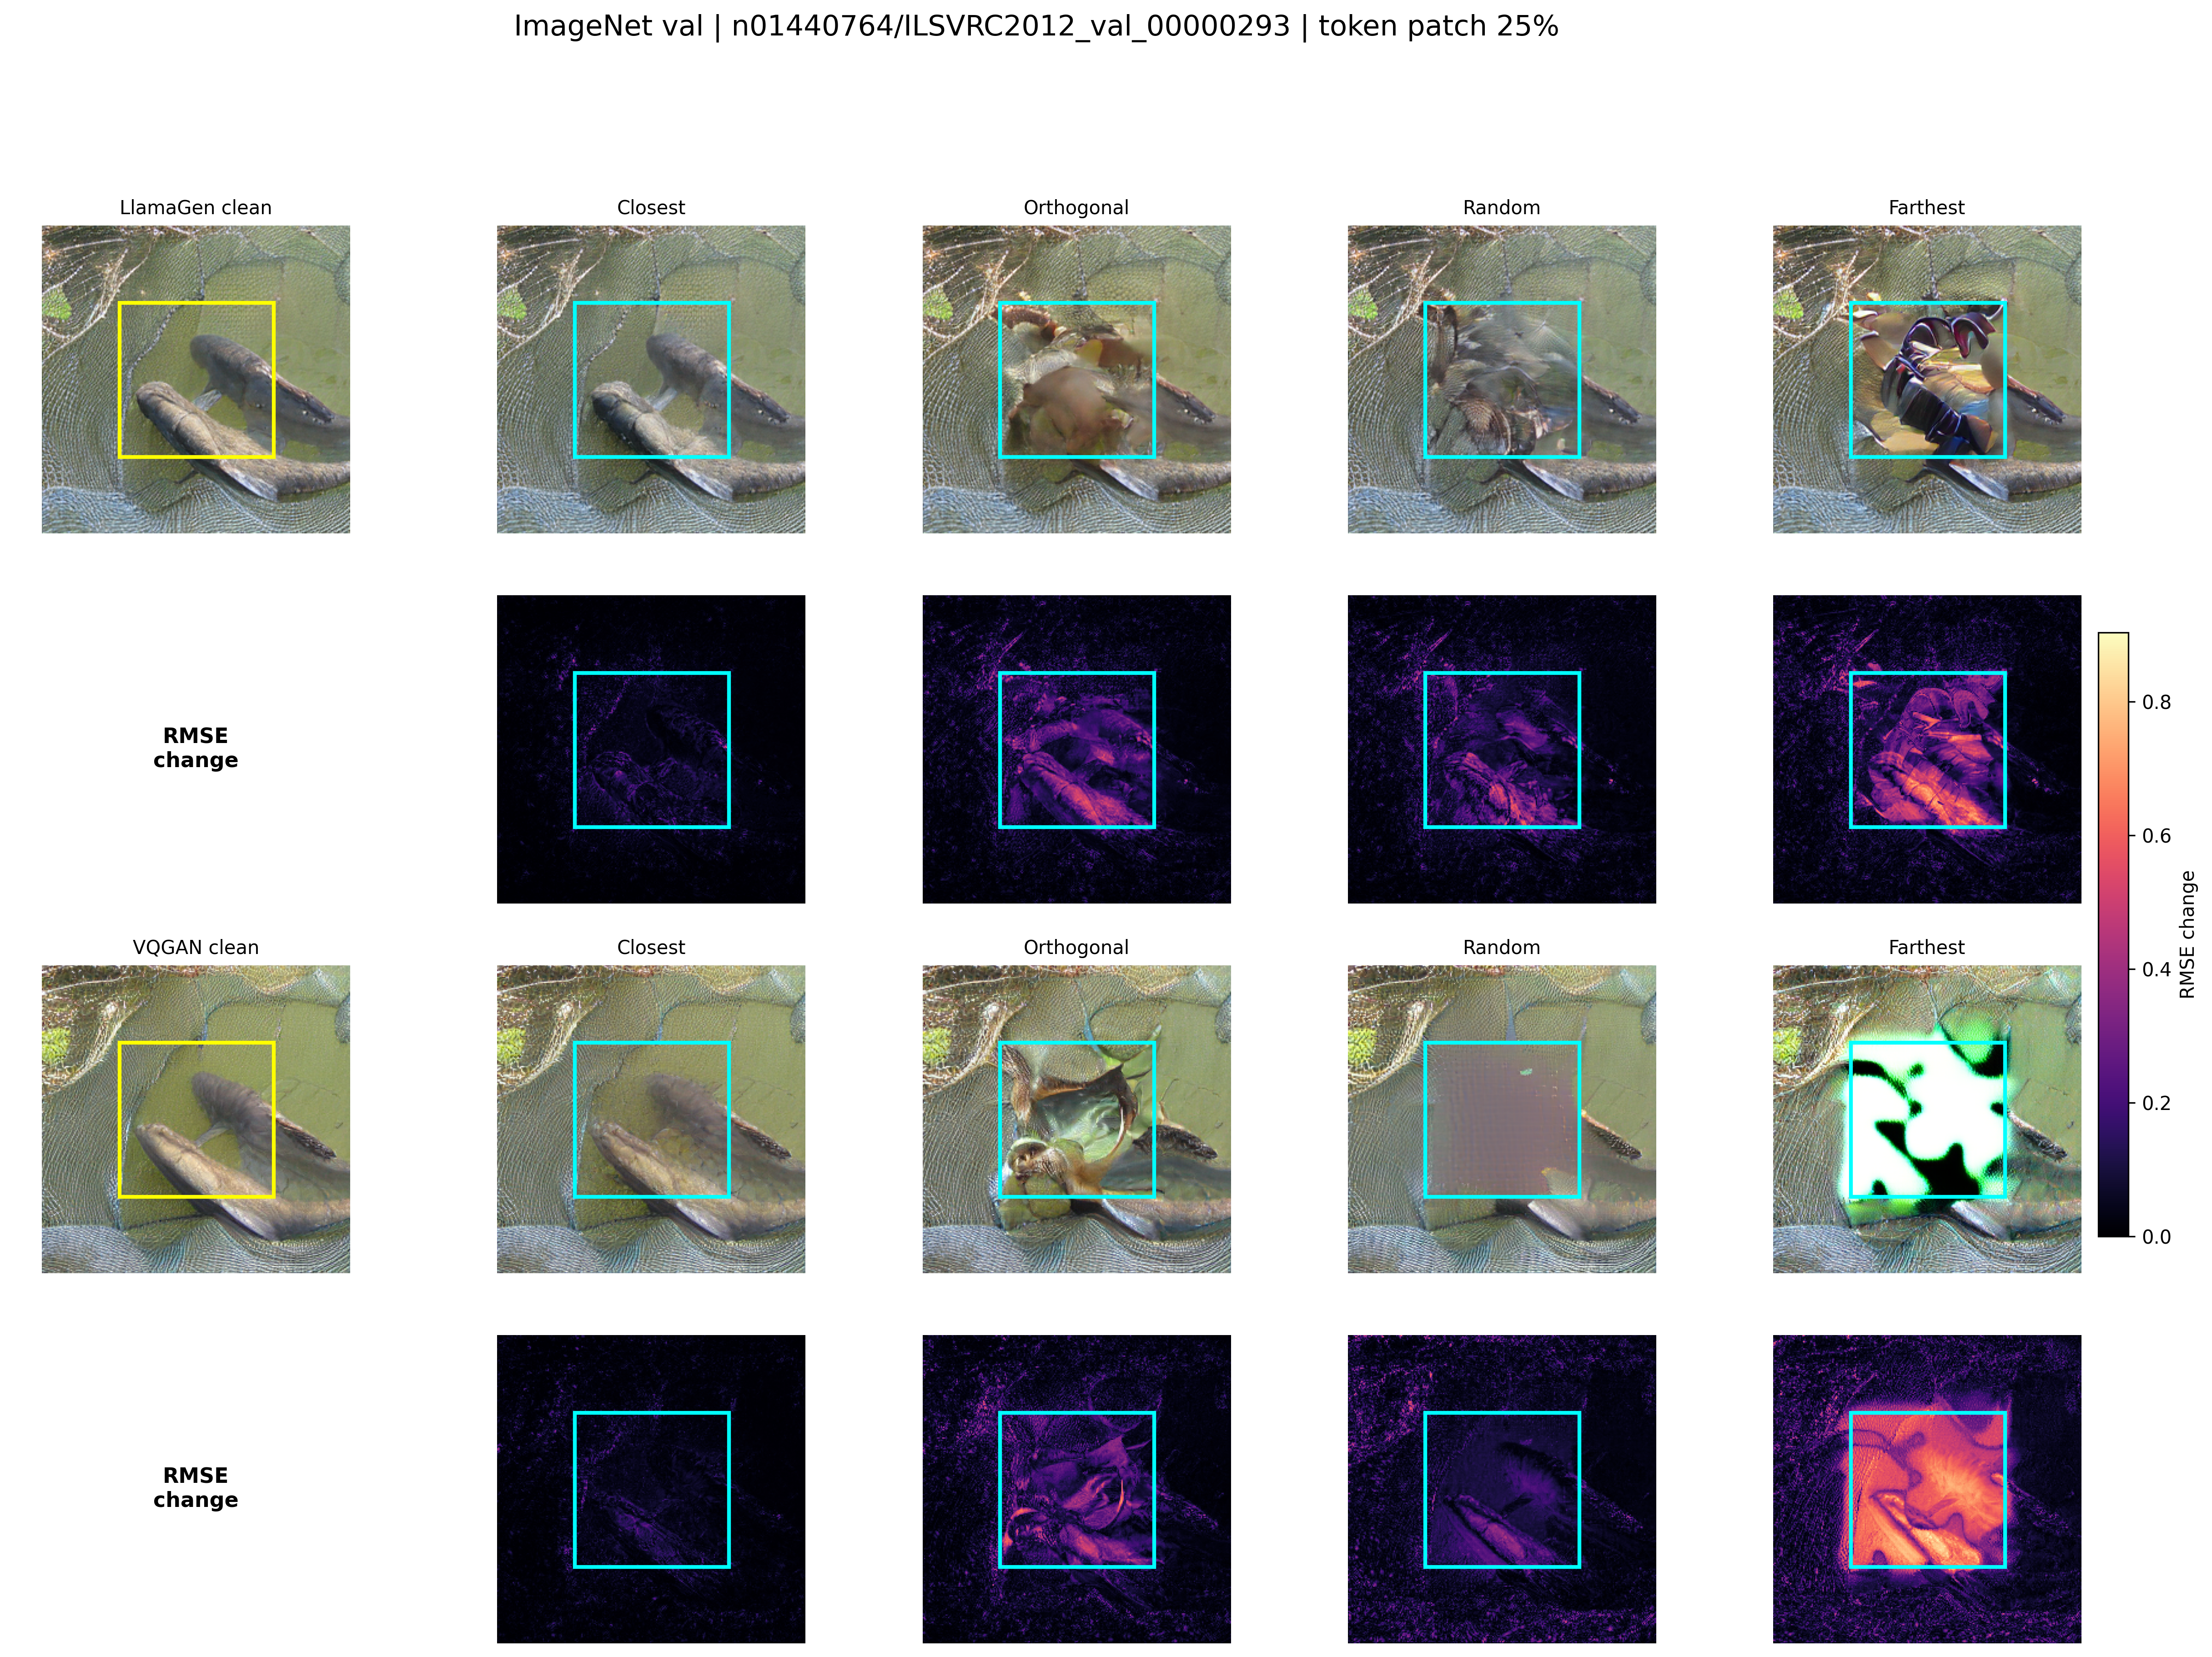
\includegraphics[width=\textwidth]{ch07_fig_token_edit_qualitative_imagenet_val_patch25.png}
    \caption{Qualitative decoder response to a 25\% token-patch perturbation.
    The cyan rectangle marks the nominal edited region. RMSE heatmaps show
    pixel change relative to each tokenizer's clean reconstruction; the figure
    should be read for the ordering of edit severity and for change outside the
    rectangle, not as a standalone quantitative result.}
    \label{fig:rq4_qualitative_token_edits}
\end{figure}
\subsection{Edit Severity}
\label{subsec:rq4_edit_severity}

Table~\ref{tab:rq4_patch25_severity} and
Figure~\ref{fig:rq4_fidelity_patch25} compare the four replacement strategies
at the 25\% patch level. Closest replacement is the mildest
intervention for both tokenizers. Its patch PSNR is 20.36 dB for LlamaGen and
20.00 dB for VQGAN, while patch LPIPS remains at 0.134 and 0.182. These edits preserve recognizable
content in Figure~\ref{fig:rq4_qualitative_token_edits}; the more distant
replacements visibly change the patch. PSNR measures pixel error, whereas
LPIPS measures differences in learned image features. Moving away
from the nearest code sharply increases perceptual change. Orthogonal
replacement raises patch LPIPS to 0.599 for LlamaGen and 0.614 for VQGAN.
The random edit should be interpreted separately from the three geometric
edits because, for VQGAN, it may sample inactive codes from the full nominal
codebook.

For LlamaGen, orthogonal and random replacement are almost indistinguishable:
their patch LPIPS values are 0.599 and 0.592, and their inside responses are
0.222 and 0.220. VQGAN behaves differently. Random replacement has a lower
mean inside RMSE than orthogonal replacement, 0.200 versus 0.239, but a much
higher patch LPIPS, 0.749 versus 0.614. The disagreement between RMSE and LPIPS
means that average pixel displacement does not account for the perceptual
effect of the VQGAN random edit.

Farthest replacement is the strongest intervention. At the 25\% level,
LlamaGen reaches a patch LPIPS of 0.702 and a patch PSNR of 7.74 dB. VQGAN is
more severely affected under its own farthest-code edit, with patch LPIPS
0.790, patch PSNR 3.74 dB, and an inside response of 0.607. Farthest-code
edits are defined separately in the two codebooks, so this is not a
severity-matched comparison of the decoders.

\begin{table}[t]
    \centering
    \small
    \begin{tabular}{llrrr}
        \textbf{Tokenizer} & \textbf{Edit mode} &
        $\boldsymbol{\Delta_{\mathrm{in}}}$ &
        \textbf{Patch PSNR} & \textbf{Patch LPIPS} \\ \hline
        LlamaGen & Closest & 0.067 & 20.36 & 0.134 \\
        LlamaGen & Orthogonal & 0.222 & 11.45 & 0.599 \\
        LlamaGen & Random & 0.220 & 11.48 & 0.592 \\
        LlamaGen & Farthest & 0.356 & 7.74 & 0.702 \\
        VQGAN & Closest & 0.072 & 20.00 & 0.182 \\
        VQGAN & Orthogonal & 0.239 & 10.66 & 0.614 \\
        VQGAN & Random & 0.200 & 12.83 & 0.749 \\
        VQGAN & Farthest & 0.607 & 3.74 & 0.790 \\
    \end{tabular}
    \caption{Edit severity for a 25\% token patch on ImageNet validation.
    Values are means over 50{,}000 images. The inside RMSE is repeated here to
    relate pixel-response magnitude to patch fidelity; the locality table also
    reports the corresponding outside response.}
    \label{tab:rq4_patch25_severity}
\end{table}
\begin{figure}[t]
    \centering
    
\includegraphics[width=\textwidth]{ch07_fig_fidelity_patch25_imagenet_val.png}
    \caption{Patch-level PSNR, SSIM, and LPIPS for the four edit modes at a
    25\% token-patch fraction.}
    \label{fig:rq4_fidelity_patch25}
\end{figure}
\begin{figure}[t]
    \centering
    
\includegraphics[width=\textwidth]{ch07_fig_patch_lpips_imagenet_val.png}
    \caption{Patch-level perceptual change as the edited token-patch fraction
    increases.}
    \label{fig:rq4_patch_lpips_sweep}
\end{figure}
Figure~\ref{fig:rq4_patch_lpips_sweep} shows that patch-level perceptual change
generally increases with patch fraction, but the edit-mode ordering remains
stable. Closest replacement stays well below the other interventions across
the sweep. For LlamaGen, orthogonal and random edits continue to track each
other closely, rising from approximately 0.51--0.52 at the 10\% level to
approximately 0.67--0.68 at 75\%. Farthest replacement remains highest,
increasing from 0.630 to 0.782.

VQGAN shows a wider separation between edit modes. Its closest-edit LPIPS
increases from 0.139 to 0.230. Random replacement rises from 0.598 to 0.879,
and overtakes farthest replacement at the 75\% level, where farthest LPIPS is
0.861. The farthest edit still has by far the largest inside RMSE response.
The two metrics rank the strongest VQGAN edit differently.

\subsection{Inside and Outside Decoder Response}
\label{subsec:rq4_inside_outside_results}

Table~\ref{tab:rq4_patch25_locality} separates the response inside the edited
region from the response outside it. At the 25\% patch level, all edit modes
produce a substantially larger mean change inside the patch. For LlamaGen,
outside response ranges from 0.013 for closest replacement to 0.050 for
farthest replacement. For VQGAN, it ranges from 0.019 to 0.090. The decoder
response is spatially concentrated, but not confined to the edited region.

The heatmaps in Figure~\ref{fig:rq4_qualitative_token_edits} show the same
pattern: the response does not stop exactly at the cyan boundary. Most change
remains within or near the edited region, but lower-amplitude changes extend
into the surrounding image, including under closest replacement.

Even nearest-neighbour replacement changes pixels outside the patch, as the
heatmaps in Figure~\ref{fig:rq4_qualitative_token_edits} also show. Farthest
replacement causes the greatest absolute change both inside and outside.
Its small ratio therefore reflects severe inside damage and should not be
read as evidence that the replacement is harmless outside the patch.

The outside response also contains localized high-amplitude changes that are
not visible from its mean alone. At the 25\% patch level, VQGAN farthest
replacement has a mean outside response of 0.090, but its mean outside 99th and
99.9th percentiles reach 0.673 and 0.854. For LlamaGen, the corresponding
values are 0.050, 0.328, and 0.554. Closest replacement has much smaller
outside tails, with 99th-percentile values of 0.105 for LlamaGen and 0.148 for
VQGAN. These tail statistics matter because mean outside response can hide
localized artifacts: strong changes can occur at a small subset of outside
pixels even when the average outside response remains low.

\begin{table}[t]
    \centering
    \small
    \begin{tabular}{llrrr}
        \textbf{Tokenizer} & \textbf{Edit mode} &
        $\boldsymbol{\Delta_{\mathrm{in}}}$ &
        $\boldsymbol{\Delta_{\mathrm{out}}}$ &
        $\boldsymbol{\widetilde{\lambda}_{\mathrm{dec}}}$ \\ \hline
        LlamaGen & Closest & 0.067 & 0.013 & 0.193 \\
        LlamaGen & Orthogonal & 0.222 & 0.039 & 0.176 \\
        LlamaGen & Random & 0.220 & 0.038 & 0.175 \\
        LlamaGen & Farthest & 0.356 & 0.050 & 0.141 \\
        VQGAN & Closest & 0.072 & 0.019 & 0.263 \\
        VQGAN & Orthogonal & 0.239 & 0.046 & 0.187 \\
        VQGAN & Random & 0.200 & 0.050 & 0.249 \\
        VQGAN & Farthest & 0.607 & 0.090 & 0.148 \\
    \end{tabular}
    \caption{Mean inside and outside response and median decoder leakage ratio
    for a 25\% token patch on ImageNet validation.}
    \label{tab:rq4_patch25_locality}
\end{table}
\begin{figure}[t]
    \centering
    
\includegraphics[width=\textwidth]{ch07_fig_decoder_locality_imagenet_val.png}
    \caption{Mean image-space response inside and outside the edited token
    patch as the patch fraction increases.}
    \label{fig:rq4_decoder_locality}
\end{figure}
\begin{figure}[t]
    \centering
    
\includegraphics[width=\textwidth]{ch07_fig_leakage_ratio_imagenet_val.png}
    \caption{Median decoder leakage ratio as a function of token-patch
    fraction and edit mode.}
    \label{fig:rq4_leakage_ratio}
\end{figure}
Figure~\ref{fig:rq4_decoder_locality} shows how these quantities change with
patch size. The mean inside response is comparatively stable for closest,
orthogonal, and farthest replacement. For example, VQGAN's farthest-edit
inside response changes only from 0.592 at the 10\% level to 0.613 at 75\%.
LlamaGen's corresponding response rises from 0.329 to 0.410. By contrast, the
outside response increases with patch size. For VQGAN farthest
replacement, the outside response rises from 0.053 to 0.213; for LlamaGen it
rises from 0.030 to 0.120.

The same growth appears in Figure~\ref{fig:rq4_leakage_ratio}. At the 75\%
level, median leakage ratios range from 0.299 to 0.418 for LlamaGen and from
0.352 to 0.531 for VQGAN. The closest and random VQGAN edits have the highest
proportional leakage at large patch sizes. The plots use median per-image
ratios throughout; near-zero inside responses can distort the mean.

\subsection{Robustness under Dataset Shift}
\label{subsec:rq4_dataset_shift}

We test ImageNet-V2 to check whether the measured decoder locality persists
beyond the in-distribution reference images. Patch-LPIPS differences from the
ImageNet validation baseline are small across both models, all four edit
modes, and all patch fractions: the largest absolute difference is 0.0068.
This is too small to support an interpretation of the individual signed
differences.

The other metrics are similarly stable. Across the full comparison, the
largest absolute change in mean outside response is 0.0016. At the 25\% patch
level, leakage-ratio differences range from $-0.0030$ to $-0.0080$, and
patch-PSNR differences remain within 0.17 dB. These differences are small
relative to those among edit modes and tokenizers. ImageNet-V2 preserves the
ordering and approximate magnitude found on ImageNet validation.
\section{Discussion}
\label{sec:rq4_discussion}

A local token-space perturbation produces a spatially concentrated decoder
response, but the response is not strictly local. Mean change is always stronger
inside the corresponding image region than outside it, and the qualitative
heatmaps preserve a clear spatial relationship to the edited patch.
Outside response is measurable even for nearest-neighbour replacement and grows as
the edited region becomes larger. Farthest-code replacement causes large
absolute changes both inside and outside the patch.

Orthogonal and random replacements are nearly equivalent for LlamaGen.
For VQGAN, random replacement is more disruptive under LPIPS than the
orthogonal edit despite a smaller average pixel response.

VQGAN random replacement can introduce codes absent from its clean ImageNet
assignments. This affects the interpretation of its scores and qualitative
examples: the experiment does not isolate the effect of distance from the
effect of using inactive codes.

The same within-checkpoint edit patterns persist across patch fractions.
At the 25\% level, the VQGAN farthest-code edit has an inside response of
0.607, compared with 0.356 for LlamaGen's separately defined farthest-code
edit; its patch PSNR is approximately 4 dB lower. These edits are not
severity-matched across codebooks, so the difference does not isolate decoder
sensitivity. Neither decoder confines the effect completely.

These decoder-side findings contrast with the encoder-side results in
Chapter~\ref{ch:rq3}. A local image-space perturbation caused widespread token
identity changes outside the patch, with outside flip rates approaching one
half under stronger perturbations. Direct token edits produce a more localized
image response: outside RMSE remains much smaller than inside RMSE.
The two experiments use different response variables, so their magnitudes are
not directly comparable. They nevertheless locate two separate effects: local
image perturbations can alter token identities far outside the patch, while
direct token edits produce a decoded response that is concentrated near the
edited region but still extends beyond it.

ImageNet-V2 preserves the same ordering and approximate response magnitude.
Decoder locality therefore persists under this mild shift to natural images
from different sources. Testing whether it persists under stronger style and
domain changes remains future work.

\chapter{Robustness to Distribution Shift}
\label{ch:rq5}

The preceding experiments measured responses to controlled noise and local
perturbations on in-distribution ImageNet images or their token grids. Inputs
encountered outside training can differ systematically in style, content, and
layout. This chapter tests whether these structured changes reduce tokenizer
robustness by evaluating six out-of-distribution datasets.
ImageNet validation remains the in-distribution reference, and six shifted
datasets vary sampling, visual style, object presentation, imaging domain, and
document layout. The experiment measures changes in global code frequency,
positional code diversity and reconstruction quality. Its
central question is whether larger changes in code usage coincide with worse
reconstruction.

Both tokenizers were trained on natural images. Chapter~\ref{ch:rq1} evaluates
them on the ImageNet validation set as the in-distribution reference. A shifted dataset can change their token
distributions in two ways. First, it may activate codes that were absent on
ImageNet, indicating that the ImageNet baseline did not expose the tokenizer's
operational vocabulary. Second, the
active vocabulary may remain fixed while assignment probabilities change,
concentrating many image patches onto a smaller effective set of codes. Raw
active-code counts detect the first failure but not the second.

Spatial allocation provides a separate view. Because each image is represented
by a $16\times16$ grid, a code can be frequent globally yet appear in different
parts of the grid under a new domain. Similarly, the range of codes observed at
a fixed grid position may contract when a dataset has strong layout regularity.
The chapter therefore separates three questions:
\begin{enumerate}
    \item Does the global code-frequency distribution change?
    \item Does code diversity change across grid positions?
    \item Are these changes accompanied by worse reconstructions?
\end{enumerate}

\section{Experimental Setup}
\label{sec:rq5_setup}

\subsection{Dataset-Shift Protocol}
\label{subsec:rq5_dataset_protocol}

The fixed reference is the 50{,}000-image ImageNet validation set. It is
compared separately with ImageNet-V2, ImageNet-Sketch, ObjectNet, OrganAMNIST,
BloodMNIST, and RVL-CDIP, using the datasets and preprocessing described in
Chapter~\ref{ch:datasets_models_metrics}. The comparison is always ImageNet
versus one shifted dataset. Table~\ref{tab:rq5_dataset_sizes} reports the number of encoded images.
Both tokenizers produce a $16\times16$ grid, giving 256 token assignments per
image.

\begin{table}[t]
    \centering
    \small
    \begin{tabular}{llr}
        \textbf{Role} & \textbf{Dataset} & \textbf{Images} \\ \hline
        ID & ImageNet & 50{,}000 \\ \hline
        OOD & ImageNet-V2 & 10{,}000 \\
        OOD & ObjectNet & 50{,}273 \\
        OOD & ImageNet-Sketch & 50{,}889 \\
        OOD & OrganAMNIST & 57{,}187 \\
        OOD & BloodMNIST & 17{,}092 \\
        OOD & RVL-CDIP & 39{,}996 \\
    \end{tabular}
    \caption{Datasets encoded for the distribution-shift analysis. ImageNet is
    the in-distribution reference for every comparison.}
    \label{tab:rq5_dataset_sizes}
\end{table}

For each tokenizer and dataset, the experiment exports the global count of
every code and a $K\times16\times16$ tensor of code counts by grid position.
The counts estimate code frequencies across the dataset and at each grid
position.

\subsection{Global Code-Usage Shift}
\label{subsec:rq5_global_metrics}

Let $p$ be the ImageNet code-frequency distribution defined in
Section~\ref{subsec:codebook_usage_metrics}, and let $q$ be the corresponding
distribution on an OOD dataset. We define two ratios for this comparison,
active-set retention and perplexity ratio, and use Jensen--Shannon divergence
as a standard measure of distribution difference.

\textbf{Active-set retention} is defined as
\begin{equation}
    \operatorname{Ret}(p,q)=
    \frac{|\{k:p_k>0\}\cap\{k:q_k>0\}|}{|\{k:p_k>0\}|}.
    \label{eq:rq5_active_retention}
\end{equation}
It measures the fraction of codes observed on the ID dataset that also occur
on the OOD dataset. Retention equals one if all ID-active codes remain active.

Perplexity is the exponential of distribution entropy,
$P(p)=\exp(H(p))$. The \textbf{perplexity ratio} is defined as
\begin{equation}
    R_P = \frac{P(q)}{P(p)}
    \label{eq:rq5_perplexity_ratio}
\end{equation}
and measures the change in effective vocabulary size. A value near one indicates
similar spread; a value below one indicates concentration onto fewer effective
codes.

The \textbf{Jensen--Shannon divergence} measures how much the probabilities of
the same code identities differ between datasets. It is defined as:
\begin{equation}
    \operatorname{JSD}(p,q)
    = \frac{1}{2}D_{\mathrm{KL}}(p\|m)
    + \frac{1}{2}D_{\mathrm{KL}}(q\|m),
    \qquad m=\frac{p+q}{2}.
    \label{eq:rq5_jsd}
\end{equation}
Here $m$ is the midpoint distribution. JSD is symmetric and remains finite
when a code appears in only one dataset; direct KL divergence need not.
It is zero for identical distributions and at most $\log 2$ with natural
logarithms. Unlike a comparison between independently sorted rank-frequency curves, this
quantity preserves code identity: probability assigned to code $k$ on
ImageNet is compared with probability assigned to the same code $k$ on the
shifted dataset. All entropy and divergence calculations use natural
logarithms, so values are reported in nats. The comparison uses $R_P$ to
measure concentration relative to each tokenizer's own ID baseline.

These global quantities pool millions of token assignments per dataset and
are therefore less sparse than the per-code positional estimates below.
Nevertheless, the datasets have unequal image counts, so small differences,
especially for ImageNet-V2 and BloodMNIST, are not treated as formal
hypothesis-test results.

\subsection{Positional Measurements}
\label{subsec:rq5_positional_metrics}

For grid position $(u,v)$, let $p_{k\mid u,v}$ be the probability of observing
code $k$ at that position over all images in a dataset. Positional entropy is
\begin{equation}
    H_{u,v}=-\sum_{k=1}^{K}p_{k\mid u,v}\log p_{k\mid u,v}.
    \label{eq:rq5_positional_entropy}
\end{equation}
We normalize entropy by $\log K$, its theoretical maximum for a codebook of
size $K$. Both checkpoints have $K=16{,}384$. The plots report the average of
$(H^{\mathrm{shift}}_{u,v}-H^{\mathrm{ImageNet}}_{u,v})/\log K$ over all
positions and separately over border and interior positions.
Negative values mean that fewer codes, or a more concentrated mix of codes,
occur at that location under the shifted dataset.

These positional entropy estimates depend on sample size. Each position
contributes one observation per image, so an empirical entropy computed from
$N$ images cannot exceed $\log(\min(K,N))$. ImageNet-V2 has 10{,}000 images,
fewer than LlamaGen's 16{,}384 codes. Its entropy difference consequently
includes a sampling effect and cannot establish a loss of intrinsic diversity.

\subsection{Reconstruction Measurements}
\label{subsec:rq5_reconstruction_metrics}

PSNR, SSIM, LPIPS, and FID are computed between each dataset and its
reconstructions under the protocol of Chapter~\ref{ch:datasets_models_metrics}.
Paired metrics are reported consistently across rows, but their magnitudes
remain sensitive to dataset content: a homogeneous medical dataset can yield
high PSNR without being close to ImageNet. FID is used only to compare the two
tokenizers on the same dataset.
Its absolute value is not compared across datasets because each row has a
different reference distribution. FID also inherits the natural-image bias of
the Inception features on which it is based; this is particularly relevant for
the medical and document datasets.

\section{Experimental Results}
\label{sec:rq5_results}

\subsection{The Active Vocabulary Is Stable but Its Distribution Is Not}
\label{subsec:rq5_global_results}

Table~\ref{tab:rq5_global_shift} reports the global code-usage measurements.
ImageNet-V2 produces almost no global shift: JSD is 0.002 for LlamaGen and
0.0004 for VQGAN, while both perplexity ratios are approximately one.
ObjectNet also remains close to the ImageNet distribution, with JSD values of
0.020 and 0.007. ImageNet-V2 contains natural images of the same classes collected from
different sources. ObjectNet changes object presentation. Both produce small
changes in the global code-frequency distribution.

\begin{table}[t]
    \centering
    \scriptsize
    \setlength{\tabcolsep}{4pt}
    \begin{tabular}{llrrr}
        \textbf{Tokenizer} & \textbf{Shifted dataset} & \textbf{Active retention} & \textbf{JSD} & $\boldsymbol{R_P}$ \\ \hline
        LlamaGen & ImageNet-V2     & 1.000 & 0.0020 & 0.995 \\
        LlamaGen & ObjectNet       & 1.000 & 0.0200 & 0.916 \\
        LlamaGen & ImageNet-Sketch & 1.000 & 0.1531 & 0.377 \\
        LlamaGen & OrganAMNIST     & 1.000 & 0.1035 & 0.624 \\
        LlamaGen & BloodMNIST      & 0.984 & 0.2260 & 0.359 \\
        LlamaGen & RVL-CDIP        & 0.994 & 0.2510 & 0.230 \\ \hline
        VQGAN & ImageNet-V2        & 1.000 & 0.0004 & 1.001 \\
        VQGAN & ObjectNet          & 1.000 & 0.0068 & 0.962 \\
        VQGAN & ImageNet-Sketch    & 1.000 & 0.1277 & 0.452 \\
        VQGAN & OrganAMNIST        & 1.000 & 0.0424 & 0.816 \\
        VQGAN & BloodMNIST         & 0.994 & 0.1575 & 0.497 \\
        VQGAN & RVL-CDIP           & 0.999 & 0.1949 & 0.325 \\
    \end{tabular}
    \caption{Global code-usage shift relative to ImageNet. Active retention is
    the fraction of ImageNet-active codes also observed on the shifted dataset;
    $R_P$ is the shifted-to-ImageNet perplexity ratio. }
    \label{tab:rq5_global_shift}
\end{table}

The style and domain changes concentrate the token distributions. RVL-CDIP gives
the largest JSD for both tokenizers, 0.251 for LlamaGen and 0.195 for VQGAN.
BloodMNIST and ImageNet-Sketch follow. Their perplexity ratios fall to
0.359--0.377 for LlamaGen and 0.452--0.497 for VQGAN. OrganAMNIST is
intermediate. The ordering is broadly shared by the two models even though
their ImageNet baselines are very different.

Active retention alone would miss this result. LlamaGen retains at least
98.4\% of its 16{,}384 ImageNet-active codes on every dataset. VQGAN retains at
least 99.4\% of its 972 ImageNet-active codes, and exactly the same 972 codes
remain active on ImageNet-V2, ImageNet-Sketch, ObjectNet, and OrganAMNIST. The
shift therefore reallocates probability among an almost unchanged vocabulary;
it does not activate ImageNet-inactive VQGAN codes at scale or collapse
LlamaGen to a small raw set.

\begin{figure}[t]
    \centering
    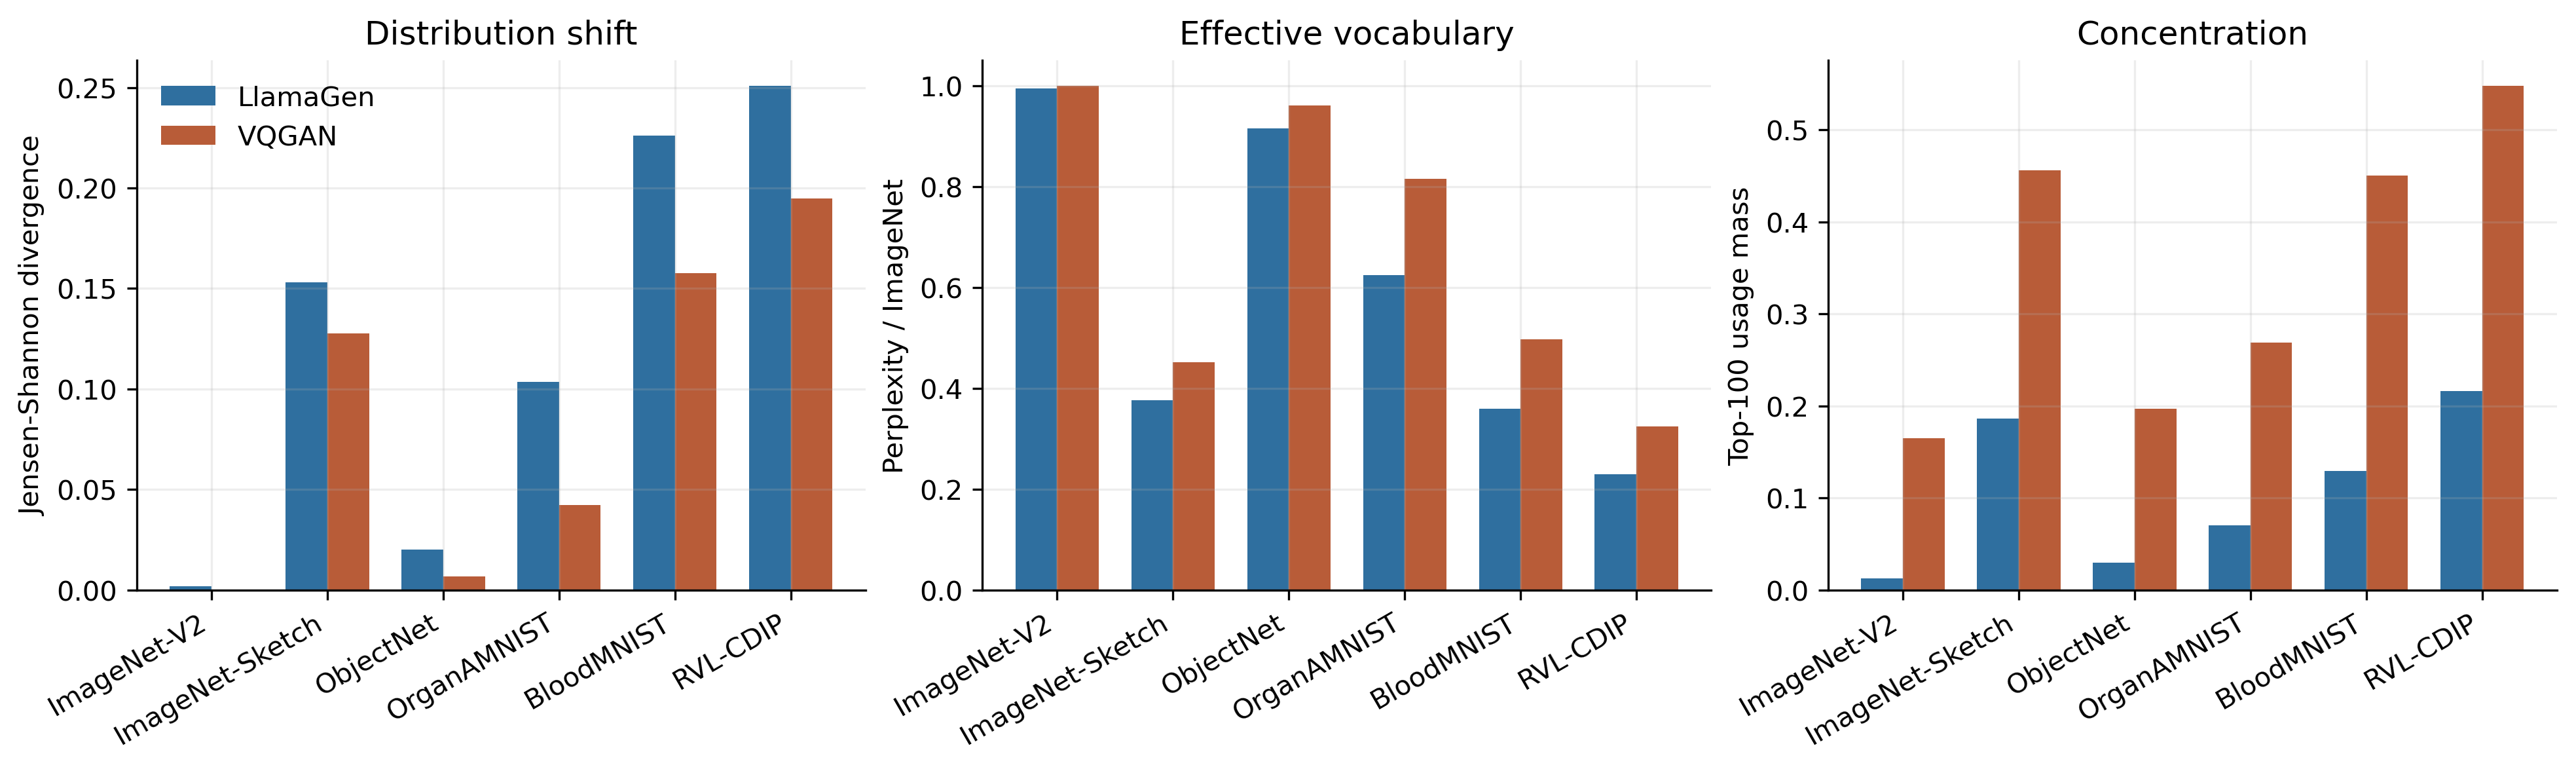
\includegraphics[width=0.98\textwidth]{ch08_fig_global_shift_summary.png}
    \caption{Global response to each shifted dataset. JSD measures movement of
    probability mass over fixed code identities; $R_P$ measures concentration relative to each tokenizer's ImageNet
    baseline.}
    \label{fig:rq5_global_shift_summary}
\end{figure}

Figure~\ref{fig:rq5_global_shift_summary} shows that ImageNet-V2 and ObjectNet
remain near the ImageNet reference. The stylized, medical, and document
datasets have lower perplexity ratios, despite little
change in their raw active sets.

\subsection{Reconstruction under Distribution Shift}
\label{subsec:rq5_reconstruction_results}

Table~\ref{tab:rq5_reconstruction_shift} reports reconstruction quality on the
six shifted datasets. LlamaGen is better in every model-paired comparison: its
PSNR and SSIM are higher, while its LPIPS and FID are lower. The advantage is
not confined to the ImageNet baseline established in
Chapter~\ref{ch:rq1}.

\begin{table}[t]
    \centering
    \scriptsize
    \setlength{\tabcolsep}{4pt}
    \begin{tabular}{llrrrr}
        \textbf{Tokenizer} & \textbf{Dataset} & \textbf{PSNR} & \textbf{SSIM} & \textbf{LPIPS} & \textbf{FID} \\ \hline
        LlamaGen & ImageNet         & 20.79 & 0.558 & 0.228 & 2.19 \\
        LlamaGen & ImageNet-V2      & 20.95 & 0.572 & 0.231 & 4.34 \\
        LlamaGen & ObjectNet        & 23.88 & 0.683 & 0.208 & 2.93 \\
        LlamaGen & ImageNet-Sketch  & 20.26 & 0.752 & 0.128 & 3.69 \\
        LlamaGen & OrganAMNIST      & 26.79 & 0.805 & 0.182 & 57.16 \\
        LlamaGen & BloodMNIST       & 27.10 & 0.802 & 0.157 & 19.60 \\
        LlamaGen & RVL-CDIP         & 20.49 & 0.764 & 0.094 & 5.08 \\ \hline
        VQGAN & ImageNet            & 19.65 & 0.489 & 0.286 & 5.06 \\
        VQGAN & ImageNet-V2         & 19.83 & 0.501 & 0.289 & 7.48 \\
        VQGAN & ObjectNet           & 22.79 & 0.611 & 0.268 & 5.80 \\
        VQGAN & ImageNet-Sketch     & 18.23 & 0.696 & 0.170 & 5.98 \\
        VQGAN & OrganAMNIST         & 26.58 & 0.732 & 0.239 & 76.12 \\
        VQGAN & BloodMNIST          & 26.38 & 0.766 & 0.201 & 29.02 \\
        VQGAN & RVL-CDIP            & 18.23 & 0.699 & 0.128 & 8.02 \\
    \end{tabular}
    \caption{Reconstruction quality on ImageNet and the shifted datasets. PSNR
    and SSIM are higher-is-better; LPIPS and FID are lower-is-better. FID
    comparisons are made between tokenizers within a dataset, not across
    dataset rows.}
    \label{tab:rq5_reconstruction_shift}
\end{table}

The paired reconstruction metrics show no uniform degradation across the
OOD datasets. ImageNet-V2 is close to ImageNet for both tokenizers.
ImageNet-Sketch has lower PSNR but higher SSIM and lower LPIPS, so the
metrics do not support a single ordering of those datasets. Medical images
have higher PSNR and SSIM and lower LPIPS than ImageNet, while document
images have higher SSIM and lower LPIPS but lower PSNR. These differences
also reflect image content and complexity. The consistent comparison is
between tokenizers on each dataset: all four metrics favor LlamaGen.

Large shifts in code frequencies can therefore coexist with preserved
reconstruction quality. FID is reported for the model comparison within each
dataset; its changing reference distribution and natural-image features
limit interpretation across domains.

\subsection{Positional Diversity Contracts under Larger Shifts}
\label{subsec:rq5_entropy_results}

Figure~\ref{fig:rq5_positional_entropy} reports normalized changes in positional
entropy on a common scale. Negative values indicate a more concentrated
distribution at a typical grid position. Comparing border and interior
averages tests whether that concentration is uniform across the grid.
These averages describe spatial variation without identifying its cause.

\begin{figure}[t]
    \centering
    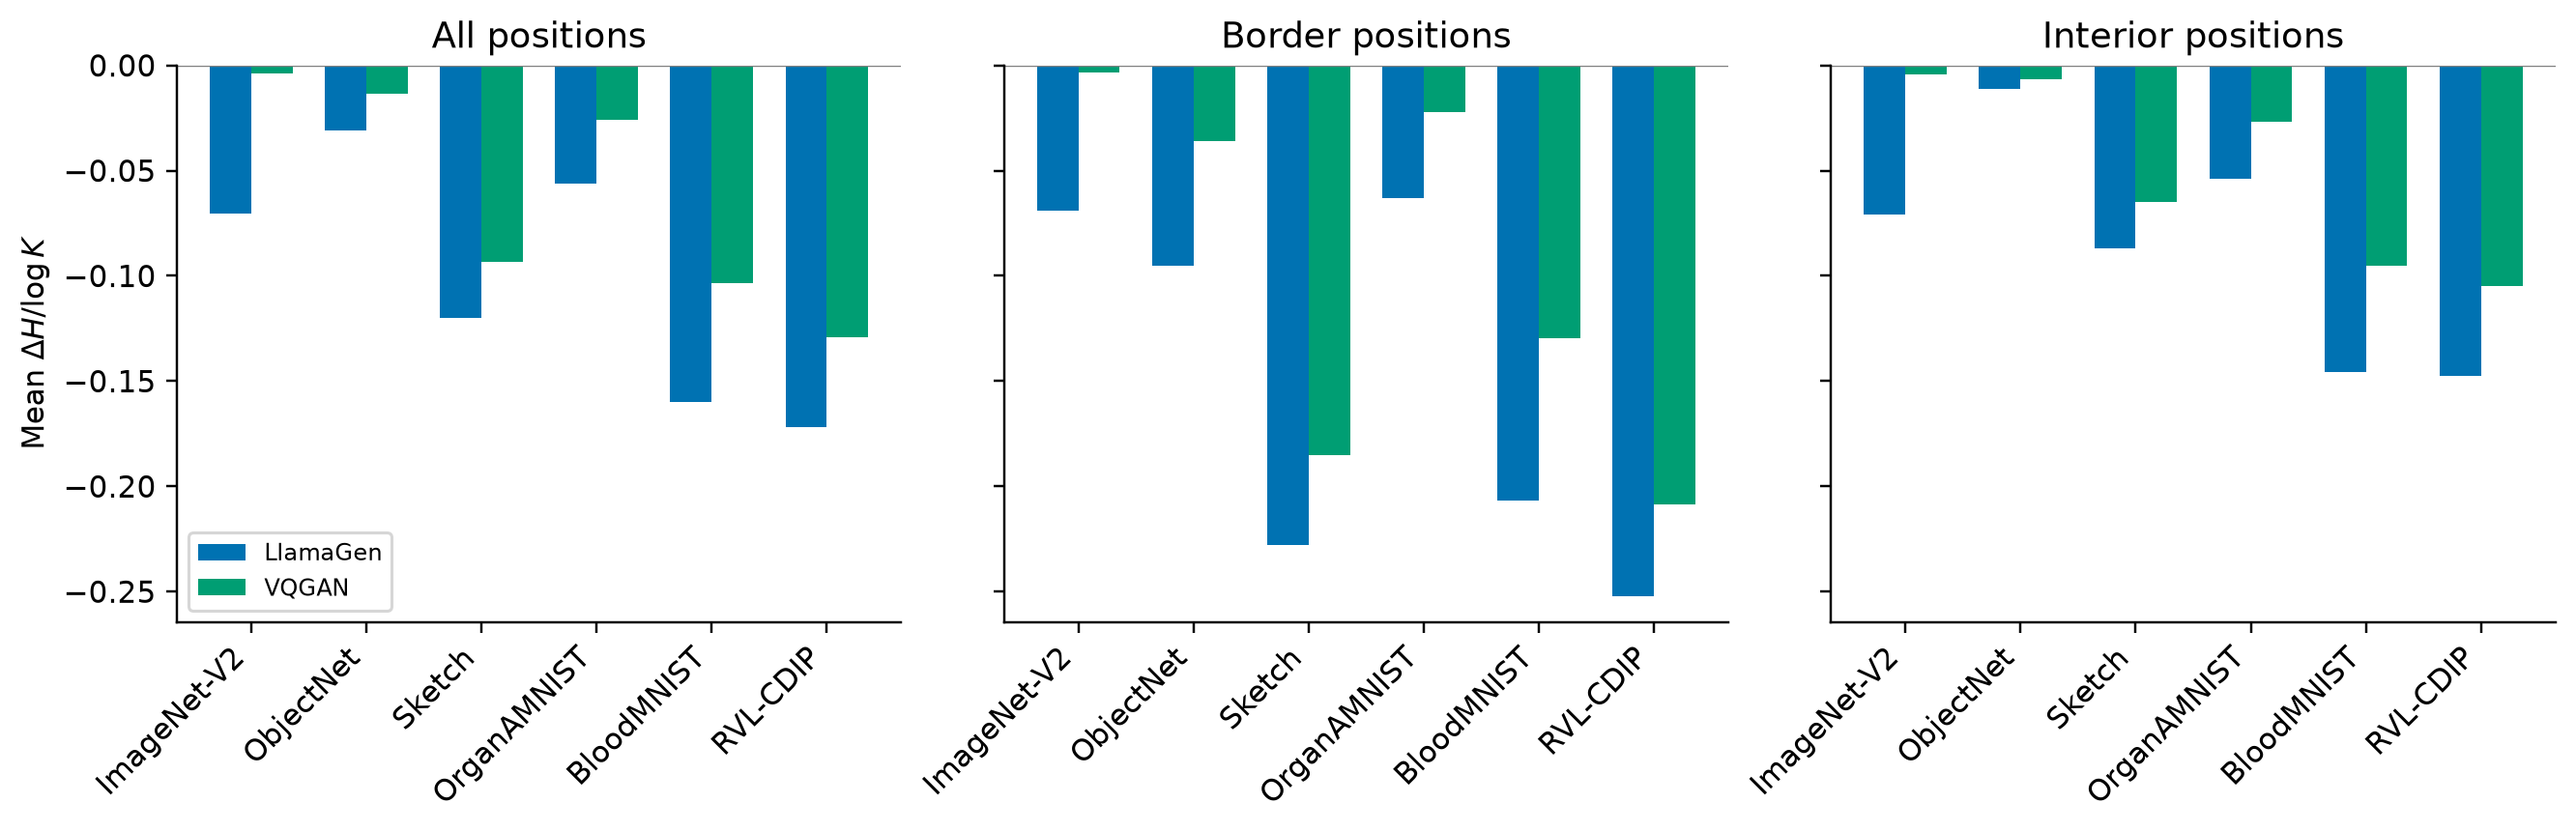
\includegraphics[width=\textwidth]{ch08_fig_normalized_positional_entropy.png}
    \caption{Mean positional entropy change divided by $\log K$, for all
    positions, border positions, and interior positions. The common scale
    expresses changes relative to the theoretical entropy range. Unequal
    dataset sizes still affect these estimates, especially ImageNet-V2.}
    \label{fig:rq5_positional_entropy}
\end{figure}

The ImageNet-V2 result illustrates why these maps require caution. Its global
distribution is almost unchanged, but LlamaGen's mean positional entropy is
0.68 lower. With only 10{,}000 images and 16{,}384 active codes, this decrease
is partly imposed by finite sampling. VQGAN, with only 972 active codes, shows
a much smaller mean decrease of 0.039. The larger decreases on datasets with
sample sizes close to ImageNet are less exposed to this specific mismatch, but
they remain empirical entropy estimates rather than intrinsic properties of
the encoder.

\section{Discussion}
\label{sec:rq5_discussion}

The distribution-shift experiment separates vocabulary availability from
vocabulary use. VQGAN's approximately 972 active ImageNet codes remain almost
exactly the active set on all six shifted datasets. LlamaGen likewise retains
nearly its full vocabulary. Neither tokenizer responds to a new domain by
substantially expanding or shrinking its raw active set. The measurable change
is redistribution: frequent codes become more dominant and perplexity falls.
Raw active-code count detects changes in vocabulary membership, but it misses
this redistribution within the active set.

ImageNet-V2 and ObjectNet remain close to the ImageNet token distribution.
Sketches, medical images, and documents use a more concentrated token mixture,
with RVL-CDIP producing the largest JSD. The two tokenizers show the same
qualitative JSD ranking despite their different empirical vocabulary sizes.

Changing the input domain substantially changes token frequencies for sketches,
medical images, and documents, while paired reconstruction scores show no
uniform decline. Both tokenizers can reconstruct images whose token
distribution differs from ImageNet. An autoregressive model trained on the
ID token distribution would receive a changed frequency distribution, with
potential consequences for its performance.

The global results are the main finding of this chapter. An almost unchanged
active vocabulary can hide substantial redistribution among its codes.
LlamaGen retains its reconstruction advantage across the tested datasets,
but its larger vocabulary does not prevent this redistribution.

% This material was merged into the final chapter. See
% Chapters/ch10_conclusion.tex, Section "Limitations and Future Work".

\chapter{Conclusion}
\label{ch:conclusion}

This thesis compared VQGAN and LlamaGen VQ-16 to determine how two pretrained
image tokenizers with the same $16\times16$ output grid differ beyond
reconstruction quality. The study measured reconstruction, empirical codebook
usage, token stability under global noise, encoder and decoder locality, and
the response to distribution shift. Each analysis isolated the tokenizer from
the autoregressive model that would consume its tokens.

The reconstruction analysis established the clean baseline and reproduced the
expected advantage of LlamaGen. On ImageNet validation, LlamaGen achieved
$20.79$ rather than $19.65$ PSNR, $0.558$ rather than $0.489$ SSIM, $0.228$
rather than $0.286$ LPIPS, and $2.19$ rather than $5.06$ FID. The codebook
measurements revealed a larger difference between the checkpoints. LlamaGen
used all 16{,}384 entries observed in this evaluation, while VQGAN used about
972. The nominal vocabulary size therefore did not describe the vocabulary
used by each checkpoint.

The analysis of global image perturbations found that neither tokenizer
preserved exact token identity under modest Gaussian noise. At $\sigma=0.1$,
79.5\% of LlamaGen positions and 75.1\% of VQGAN positions differed from their
clean assignments. The decoded images still retained their broad visual
structure, and LlamaGen kept its reconstruction advantage at every tested
noise level. Token assignments can therefore change much faster than the
reconstructed image. Noise also concentrated code usage in both models without
greatly changing the raw number of active codes.

The analysis of local image perturbations found that the encoder response was
not confined to the perturbed patch. At low patch noise, the far-field token
flip rate was 17.4\% for VQGAN and 17.8\% for LlamaGen. Masking one image patch
changed 56.3\% of VQGAN positions and 49.5\% of LlamaGen positions outside the
corresponding token region. A local change in image space can therefore alter
the discrete representation well beyond that region.

The decoder analysis found a more concentrated response. Directly editing a
local token patch produced the largest pixel changes near the edited region,
although measurable changes remained outside it. The same pattern held on the
slightly out-of-distribution ImageNet-V2 dataset, where the largest change in
patch LPIPS relative to ImageNet validation was 0.0068. Locality is therefore
preserved approximately rather than exactly when the decoder maps token edits
back to pixels.

When tested on out-of-distribution datasets, both VQGAN and LlamaGen retained
almost all codes that were active on ImageNet. They did not switch to a
substantially different set of active tokens. Instead, they changed how often
they used those tokens. ImageNet-V2 and ObjectNet remained close to the
ImageNet token distribution, while sketches, medical images, and document
pages produced larger changes. RVL-CDIP produced the largest
Jensen--Shannon divergence for both tokenizers. Even these large changes in
token frequency did not consistently produce large losses in paired
reconstruction quality.

Overall, better reconstruction and broader codebook usage did not imply greater
stability under noise. LlamaGen reconstructed images more accurately and used
far more codes, yet its token assignments changed at a rate similar to VQGAN's.
The distribution-shift results point to the same distinction. Large changes in
the token stream can coexist with modest changes in reconstruction. A
tokenizer therefore determines more than how faithfully an image is rebuilt;
it also determines the sequence distribution presented to the autoregressive
model.

\section{Limitations and Future Work}
\label{sec:limitations_future_work}

This study compared one pretrained VQGAN checkpoint with one pretrained
LlamaGen VQ-16 checkpoint. Because the models differ in architecture, training
procedure, objective, codebook dimensionality, and normalization, the observed
differences describe the two complete systems. They do not identify which
design choice caused each result. A direct mechanistic study should modify one
tokenizer property at a time, retrain the affected models, and repeat the same
measurements. This would separate the effects of codebook size, training
objective, and architecture.

Both tokenizers also require a fixed $256\times256$ input. Resizing and cropping
can alter datasets whose native resolution, aspect ratio, or layout differs
from ImageNet, especially document and medical images. Future comparisons
should include tokenizers with adaptive input resolution and test whether the
same distribution-shift patterns remain without a fixed-size preprocessing
step.

The analyses of global and local perturbations used the same seeds and
intervention levels for both models, but they did not save a shared manifest of
the exact noise arrays and patch locations. This avoidable limitation was
identified after data collection. A replication should export every
intervention once and apply the same saved intervention to both tokenizers.

Finally, the study did not train or evaluate an autoregressive model on the
measured token streams. It therefore cannot show how token instability,
concentrated code usage, or distribution-dependent token frequencies affect
generation. Future work should train or evaluate autoregressive priors on these
streams and measure generation quality and robustness directly. The spatial
analysis should also be repeated with matched dataset sizes, since unequal
sample counts affect the current positional-entropy estimates.


% --------------------------------------------------------------------------
% APPENDICES
% --------------------------------------------------------------------------
\appendix
\chapter{Implementation and Code Organization}
\label{app:implementation_code_organization}

\section{Repository Structure}
\label{sec:appendix_repositories}

The experimental implementation is divided across three repositories. The
\texttt{taming-transformers} repository contains the VQGAN model and its
experiment scripts~\cite{tamingtransformersgithub}, while \texttt{LlamaGen}
contains the corresponding tokenizer implementation~\cite{llamagengithub}.
The \texttt{vq-explore} repository contains the
comparative analysis notebooks and the decoder-locality analysis utility. This
separation keeps model-specific inference code close to each model while
placing cross-model analysis in one location.

\section{Experiment Scripts}
\label{sec:appendix_experiment_scripts}

Equivalent scripts were implemented for the two tokenizers. The reconstruction
scripts encode and decode image-folder datasets and export per-image fidelity
metrics and reconstructed images. The code-usage scripts accumulate global and
position-dependent token counts. The robustness exporters implement the three
interventions used in this thesis: global Gaussian noise, local image-space
patch perturbations, and local token-space replacement.

For each robustness run, images are processed in batches on the GPU. Image
writing and metadata export are delegated to worker processes so that disk
operations do not block inference. Each sample is stored under its dataset
class and image identifier. Sharded JSONL metadata records the perturbation
parameters, patch coordinates, and clean and perturbed token grids. This format
allows later analyses to recompute metrics without rerunning either tokenizer.

The token-space experiments additionally require mappings from each token to a
closest, farthest, and approximately orthogonal alternative. LlamaGen mappings
are computed over its full, L2-normalized codebook. VQGAN mappings are computed
over the empirically active subset used by the experiment, as described in
Chapter~\ref{ch:rq4}.

\section{Analysis Notebooks and Outputs}
\label{sec:appendix_notebook_analysis}

One notebook consolidates the analysis for each experimental chapter:
\texttt{ch04\_rq1\_reconstruction\_codebook\_usage.ipynb},
\texttt{ch05\_rq2\_global\_robustness.ipynb},
\texttt{ch06\_rq3\_local\_image\_perturbations.ipynb},
\texttt{ch07\_rq4\_token\_space\_perturbations.ipynb}, and
\texttt{ch08\_rq5\_distribution\_shift.ipynb}. The notebooks read the
exported images and metadata, compute chapter-level summaries, and save the
tables and figures cited in the thesis. Expensive per-image calculations are
cached as CSV, Parquet, or NPZ files where appropriate. CPU-bound image metrics
are parallelized across workers, while LPIPS is evaluated in GPU batches.

On the analysis host, chapter outputs follow a common layout:
\texttt{chapterN\_outputs/data} contains summary tables,
\texttt{chapterN\_outputs/figures} contains plots, and
\texttt{chapterN\_outputs/qualitative\_samples} contains the source images used
for visual comparisons. Compact source artifacts are copied into
\texttt{Assets/rqN/data} and \texttt{Assets/rqN/figures} in the thesis
repository, where \texttt{rqN} denotes the research-question number. Figures
included by LaTeX are copied into \texttt{Images}. Raw reconstructions and
complete run exports remain outside the thesis repository.

\section{Reproducibility Record}
\label{sec:appendix_reproducibility}

The file \texttt{Assets/reproducibility\_manifest.csv} records the repository
revision, working-tree state, and SHA-256 digest of each experiment script and
analysis notebook in the audited snapshot. The revision identifies the last
commit that changed the file. The digest identifies its exact local contents.
Most entries match their committed revision. The two reconstruction exporters
and the RQ2 notebook contain later uncommitted changes, so the manifest marks
them as modified rather than presenting the listed commit as an exact snapshot.

Both tokenizers process RGB images at $256\times256$ resolution using a
shortest-side resize followed by a center crop. Both expose a nominal
16{,}384-entry codebook and produce a $16\times16$ token grid. The VQGAN runs
load \texttt{/checkpoints/vqgan\_imagenet\_f16\_16384/model.yaml} and
\texttt{last.ckpt}; the LlamaGen runs load
\texttt{/checkpoints/vq\_ds16\_c2i.pt} with the VQ-16 architecture, embedding
dimension 8, and codebook size 16{,}384. Robustness exporters set the Python,
NumPy, and PyTorch random seeds to 0. Code-usage exports are deterministic with
respect to input order: class directories and file names are sorted, data
loading uses \texttt{shuffle=False}, and no token sampling is performed.

For each code-usage run, \texttt{global\_counts.npy} stores one count per
codebook index and \texttt{position\_counts.npy} stores counts with shape
$K\times16\times16$. The exporter also writes \texttt{usage.csv}, the 500 most
frequent codes, and \texttt{summary.json}. When enabled,
\texttt{indices.npz} stores one token grid and source path per image. The
Chapter~\ref{ch:rq5} artifact inventory verifies image counts, token-grid shape,
total token counts, and active-code counts for every model--dataset pair. These
checks are archived in \texttt{Assets/rq5/data/ch08\_artifact\_inventory.csv}.

\chapter{Computational Environment}
\label{app:computational_environment}

\section{Containerized Execution}
\label{sec:appendix_containerized_execution}

The two tokenizer implementations have incompatible software requirements and
were therefore executed in separate Docker images on a CUDA-enabled server.
The ImageNet datasets and pretrained checkpoints were mounted into the
containers, while experiment directories were mounted into persistent storage.
Long-running full-dataset exports were launched in background terminal
sessions. Random seeds, perturbation modes, patch sizes, and output locations
were fixed by script arguments or environment variables and recorded in run
directory names and metadata.

\section{Tokenizer Environments}
\label{sec:appendix_tokenizer_environments}

The VQGAN environment is based on Ubuntu 20.04 with CUDA 11.7, Python 3.8,
PyTorch 1.13.1, and torchvision 0.14.1. It retains the older dependencies
required by Taming Transformers, including PyTorch Lightning 1.0.8,
OmegaConf 2.0.0, and scikit-image 0.18.3.

The LlamaGen environment uses Ubuntu 20.04 with CUDA 12.2, PyTorch 2.1.2, and
torchvision 0.16.2. Its analysis dependencies include NumPy, Pillow,
scikit-image, pandas, Matplotlib, and LPIPS. Both environments expose the same
dataset and checkpoint mounts, allowing the model-specific exporters to
produce compatible image and metadata layouts.

The model exporters do not use byte-identical resizing operators. LlamaGen
repeatedly downsamples large images with Pillow BOX filtering, resizes the
shortest side with bicubic interpolation, and then applies an integer center
crop. The VQGAN exporter resizes the shortest side with Lanczos interpolation
before center cropping. Both produce RGB $256\times256$ tensors, but this
filtering difference is a preprocessing confound in fine-grained cross-model
comparisons.

\section{Evaluation and Analysis Environment}
\label{sec:appendix_evaluator_environment}

Distribution-level reconstruction metrics are computed in a separate
evaluator image containing TensorFlow CPU 2.9, PyTorch, torchvision, and
\texttt{torch-fidelity}. Reconstructions are exported as uint8 NPZ arrays and
compared with reference statistics generated from the same ImageNet validation
preprocessing. Using a separate evaluator avoids changing either tokenizer
environment solely to satisfy metric dependencies.

The chapter notebooks run in the Jupyter environment associated with
\texttt{vq-explore}. They use pandas and NumPy for aggregation, Matplotlib for
figures, scikit-image for pixel metrics, and batched LPIPS evaluation where
required. Full ImageNet experiments use 50{,}000 validation images. DataLoader
workers, asynchronous image writers, process pools, and GPU metric batches are
used to keep model inference and analysis practical without changing the
experimental definitions.

The exact GPU model and wall-clock duration of every historical run were not
archived consistently and are therefore not reconstructed here. Container
versions, checkpoints, seeds, scripts, and compact outputs are retained; the
omitted hardware timing details do not affect the numerical definitions of the
reported metrics.


% REFERENCES
\cleardoublepage
\bibliography{Thesis_bibliography}

% LIST OF FIGURES
\cleardoublepage
\listoffigures

% LIST OF TABLES
\cleardoublepage
\listoftables

% LIST OF SYMBOLS
\cleardoublepage
\chapter*{List of Symbols}
\addcontentsline{toc}{chapter}{List of Symbols}
\begin{longtable}{p{0.20\textwidth}p{0.70\textwidth}}
    \textbf{Symbol} & \textbf{Description} \\ \hline
    $x$ & Input image. \\[2px]
    $\hat{x}$ & Reconstructed image. \\[2px]
    $x_{\sigma}$ & Image perturbed by Gaussian noise with standard deviation $\sigma$. \\[2px]
    $E$, $Q$, $D$ & Encoder, vector quantizer, and decoder. \\[2px]
    $z_e$, $z_q$ & Continuous encoder output and quantized latent representation. \\[2px]
    $z_0$, $z_{\sigma}$ & Clean and perturbed discrete token grids. \\[2px]
    $e_k$ & Embedding vector associated with codebook entry $k$. \\[2px]
    $K$ & Nominal codebook size. \\[2px]
    $h,w$ & Height and width of the token grid. \\[2px]
    $p_k$ & Empirical assignment probability of codebook entry $k$. \\[2px]
    $H(p)$ & Entropy of the empirical token distribution. \\[2px]
    $\operatorname{PPL}$ & Effective codebook perplexity, $\exp(H(p))$. \\[2px]
    $\sigma$ & Standard deviation of an applied Gaussian perturbation. \\[2px]
    $M_P$ & Binary image-space mask for patch $P$. \\[2px]
    $I_P$, $O_P$ & Token positions inside and outside patch $P$. \\[2px]
    $R_{\mathrm{in}}$, $R_{\mathrm{out}}$ & Mean encoder-side token response inside and outside a perturbed patch. \\[2px]
    $\lambda_{\mathrm{enc}}$ & Encoder leakage ratio, $R_{\mathrm{out}}/(R_{\mathrm{in}}+\varepsilon)$. \\[2px]
    $B_{\mathrm{tok}}$, $B_{\mathrm{px}}$ & Edited token-space region and its corresponding image-space region. \\[2px]
    $\Delta_{\mathrm{in}}$, $\Delta_{\mathrm{out}}$ & Mean decoder-side image response inside and outside an edited region. \\[2px]
    $\lambda_{\mathrm{dec}}$ & Decoder leakage ratio, $\Delta_{\mathrm{out}}/(\Delta_{\mathrm{in}}+\varepsilon)$. \\[2px]
    $\varepsilon$ & Fixed small positive constant that prevents division by zero in leakage ratios. \\[2px]
\end{longtable}

% ACKNOWLEDGEMENTS
\chapter*{Acknowledgements}
I thank Professor Matteo Matteucci for his supervision and Paolo Cudrano for
his guidance and support throughout this work.

\cleardoublepage

\end{document}
